\documentclass[12pt]{ociamthesis}  % default square logo 
%\documentclass[12pt,beltcrest]{ociamthesis} % use old belt crest logo
%|\documentclass[12pt,shieldcrest]{ociamthesis} % use older shield crest logo

\usepackage{lipsum}
\usepackage{setspace}

%load any additional packages
\usepackage{amssymb}
\usepackage{amsmath}
%\usepackage{url}
\usepackage[toc,page]{appendix}
\usepackage[font={small}]{caption}
\usepackage{subcaption}
%\usepackage{subfig}
\usepackage{subfloat}
\usepackage[usestackEOL]{stackengine}
\usepackage{epigraph}
\usepackage{multirow}
\def\changemargin#1#2{\list{}{\rightmargin#2\leftmargin#1}\item[]}
\let\endchangemargin=\endlist

\usepackage{soul}
\DeclareRobustCommand{\hlgr}[1]{{\sethlcolor{green}\hl{#1}}}
\usepackage[T1]{fontenc}

\usepackage[bottom]{footmisc}
\usepackage[framemethod=tikz]{mdframed}
\usepackage{enumitem}

\usepackage{graphicx}
\graphicspath{{./figures/}}
\DeclareGraphicsExtensions{.pdf,.png, .gif, .jpg}

\usepackage{dirtree}
\renewcommand*\DTstylecomment{\rmfamily\color{red}\textsc}
%\renewcommand{\DTstyle}{\textrm\expandafter\raisebox{-0.3ex}}
\DTsetlength{0.5em}{0.5em}{0.2em}{0.2pt}{0.2pt}
%\setlength{\DTbaselineskip}{2\baselineskip}

\usepackage{tikz-qtree}
\usepackage{forest}
\usepackage{makecell}
\usepackage{xcolor}
\usepackage{colortbl}
\usepackage{fixltx2e}
\usepackage{rotating}
\newcommand{\anything}{\mathbin{\rotatebox[origin=c]{90}{$\lozenge$}}}
\newcommand{\nothing}{\text{\rule{1.5ex}{0.4pt}\;}}
\newcommand{\Sub}{\rule{1ex}{0.4pt}}

\usepackage{array}
\newcolumntype{M}[1]{>{\arraybackslash}m{#1}}
\newcolumntype{N}{@{}m{0pt}@{}}

\usepackage{pgfplots, pgfplotstable}
\pgfplotstableread[col sep = semicolon]{figures/chapter5/accuracy_data.csv}\mydata

\usepackage{tikz-dependency}
%\tikzset{/depgraph/.cd,/depgraph/.search also = {/tikz},
%    baseline=-0.6ex, inner sep=-0.1cm, edge horizontal padding=3pt, edge unit distance=1.5ex}

% ========== AUTOMATIC CELL COLOURING =====%
\makeatletter
\newcommand*{\minuscellcolor}{}
\def\minuscellcolor\ignorespaces{%
  % \ignorespaces not really needed, because \@ifnextchar gobbles spaces
  \@ifnextchar-{\cellcolor{red}}{}%
}

\makeatother

% ========== ALGORITHMS CUSTOMIZATION ==== %

\usepackage{algorithm}
\usepackage[noend]{algpseudocode}
\newcommand*\Arg{\textit}
\newcommand*\func{\textsc}

\usepackage{caption}
\makeatletter
\@addtoreset{algorithm}{chapter}% algorithm counter resets every chapter
\makeatother
\renewcommand{\thealgorithm}{\thechapter.\arabic{algorithm}}% Algorithm # is <chapter>.<algorithm>


\newcommand*\Let[2]{\State #1 $\gets$ #2}
\colorlet{kw}{blue}
\colorlet{rd}{red}
\definecolor{com}{rgb}{0,0.6,0}

% redefine keywords
\algrenewcommand\algorithmicfunction{\textcolor{kw}{\textbf{function}}}
\algrenewcommand\algorithmicwhile{\textcolor{kw}{\textbf{while}}}
\algrenewcommand\algorithmicfor{\textcolor{kw}{\textbf{for}}}
\algrenewcommand\algorithmicif{\textcolor{kw}{\textbf{if}}}
\algrenewcommand\algorithmicelse{\textcolor{kw}{\textbf{else}}}
\algrenewcommand\algorithmicend{\textcolor{kw}{\textbf{end}}}
\algrenewcommand\algorithmicreturn{\textcolor{kw}{\textbf{return}}}
\algrenewcommand\algorithmicthen{\textbf{then}}

\algnewcommand\IF{\If}

% new keywords
\algnewcommand\Break{\textbf{\textcolor{kw}{break}}}%
\algnewcommand\Continue{\textcolor{kw}{continue}}%
\algnewcommand\Each{\textbf{\textrm{each }}}%
\algnewcommand\In{\textbf{\textrm{ in }}}%
\algnewcommand\True{\textcolor{rd}{\textbf{true}}}%
\algnewcommand\False{\textcolor{rd}{\textbf{false}}}%
\algnewcommand\Null{\textcolor{rd}{\textbf{null}}}
\algnewcommand\Or{\textbf{or }}

% redefine loops
\algdef{SE}[WHILE]{While}{EndWhile}[1]{\algorithmicwhile\ #1}{\algorithmicend}%
\algdef{SE}[FOR]{For}{EndFor}[1]{\algorithmicfor\ #1}{\algorithmicend}%
\algdef{C}[IF]{IF}{ElsIf}[1]{\algorithmicelse\algorithmicif\ #1}%

% redefine comments
%\algrenewcommand{\algorithmiccomment}[1]{{\color{com}#1}}


% =========== CUSTOM LSTLISTINGS ====== %

\usepackage{listings}
\definecolor{codegreen}{rgb}{0,0.6,0}
\definecolor{codegray}{rgb}{0.5,0.5,0.5}
\definecolor{codepurple}{rgb}{0.58,0,0.82}
\definecolor{backcolour}{rgb}{0.97,0.97,0.97}

\usepackage{inconsolata}
\lstset{
  basicstyle=\ttfamily,
}
 
\lstdefinestyle{mystyle}{
	basicstyle=\footnotesize\ttfamily,
    backgroundcolor=\color{backcolour},   
    commentstyle=\color{codegreen},
    keywordstyle=\color{magenta},
    numberstyle=\tiny\color{codegray},
    stringstyle=\color{codepurple},
    basicstyle=\footnotesize,
    breakatwhitespace=false,         
    breaklines=true,                 
    captionpos=b,                    
    keepspaces=true,                 
    numbers=left,                    
    numbersep=5pt,                  
    showspaces=false,                
    showstringspaces=false,
    showtabs=false,
    frame=lines,                  
    tabsize=2    
}

\colorlet{punct}{red!60!black}
\definecolor{delim}{RGB}{20,105,176}
\definecolor{mypink}{RGB}{221,54,149}
\colorlet{numb}{magenta!60!black}

\newcommand\JSONnumbervaluestyle{\color{blue}}
\newcommand\JSONstringvaluestyle{\color{mypink}}

% switch used as state variable
\newif\ifcolonfoundonthisline

\makeatletter

\lstdefinelanguage{json}
{
	literate=
		{:}{{{\color{punct}{:}}}}{1}
		{,}{{{\color{punct}{,}}}}{1}
		{\{}{{{\color{delim}{\{}}}}{1}
		{\}}{{{\color{delim}{\}}}}}{1}
		{[}{{{\color{delim}{[}}}}{1}
		{]}{{{\color{delim}{]}}}}{1},
	showstringspaces    = false,
	keywords            = {false,true},
	alsoletter          = 0123456789.,
	morestring          = [s]{"}{"},
	stringstyle         = \ifcolonfoundonthisline\JSONstringvaluestyle\fi,
	MoreSelectCharTable =%
		\lst@DefSaveDef{`:}\colon@json{\processColon@json},
	morecomment=[l]{//}
}

\lstdefinelanguage{JavaScript}{
  keywords={typeof, new, true, false, catch, function, return, null, catch, switch, var, if, in, while, do, else, case, break},
  keywordstyle=\color{blue}\bfseries,
  ndkeywords={class, export, boolean, throw, implements, import, this},
  ndkeywordstyle=\color{darkgray}\bfseries,
  identifierstyle=\color{black},
  sensitive=false,
  comment=[l]{//},
  morecomment=[s]{/*}{*/},
  commentstyle=\color{com}\ttfamily,
  stringstyle=\color{red}\ttfamily,
  morestring=[b]',
  morestring=[b]"
}

\lstdefinelanguage{Rules}{
    literate=
		{->}{{{\color{blue}{->}}}}{1}
		{<}{{{\color{red}{<}}}}{1}
		{>}{{{\color{red}{>}}}}{1}
		{_}{{{\color{red}{\_}}}}{1}
		{|}{{{\color{blue}{|}}}}{1},
  identifierstyle=\color{black},
  sensitive=false,
  comment=[l]{//},
  commentstyle=\color{com}\ttfamily
}

\lstdefinelanguage{Rules2}{
    literate=
		{->}{{{\color{blue}{->}}}}{1}
		{_}{{{\color{blue}{\_}}}}{1},
  keywords={SWAP, TAG, WORDS, DT, PRP,POS,IN,MD,NNS,NN,CC,\$,RB,VB,VBD,VBZ,VBG,VBP},
  keywordstyle=\color{red}\bfseries,
  identifierstyle=\color{black},
  sensitive=false,
  comment=[l]{//},
  commentstyle=\color{com}\ttfamily
}

% flip the switch if a colon is found in Pmode
\newcommand\processColon@json{%
  \colon@json%
  \ifnum\lst@mode=\lst@Pmode%
    \global\colonfoundonthislinetrue%
  \fi
}

\lst@AddToHook{Output}{%
  \ifcolonfoundonthisline%
    \ifnum\lst@mode=\lst@Pmode%
      \def\lst@thestyle{\JSONnumbervaluestyle}%
    \fi
  \fi
  %override by keyword style if a keyword is detected!
  \lsthk@DetectKeywords% 
}

% reset the switch at the end of line
\lst@AddToHook{EOL}%
  {\global\colonfoundonthislinefalse}

\makeatother

\lstset{style=mystyle}
\lstset{basicstyle=\footnotesize\ttfamily}

%======= custom overline ====== %
\newcommand{\tolstrut}{%
  \vrule height\dimexpr\fontcharht\font`\A+.7ex\relax width 0pt\relax
}

\DeclareRobustCommand{\ovl}[1]{%
  \ensuremath{\overline{\mbox{\tolstrut#1}}}%
}

%============ BIBLIOGRAPHY AND REFS PACKAGES ========%
\usepackage[numbers]{natbib}
\usepackage{multibib}
\newcites{x}{References}
\newcites{sec}{Background Reading}

%============ for gloss overline ========%
\makeatletter
\newcommand{\OVER}[1]{$\overline{\hbox{#1}}\m@th$}
\makeatother

\newcommand{\TAG}{\textsuperscript}
\newcommand{\SUB}{\textsubscript}

\usepackage{slgloss}

% ========= for table stuff
\newcommand\Tstrut{\rule{0pt}{2.6ex}}       % "top" strut

% ========= for general formatting of text
\newcommand{\tech}{\texttt}

% ============== stuff below is for header\footer
\usepackage{fancyhdr}
\pagestyle{fancy}
\fancyhead{}
\renewcommand{\sectionmark}[1]{\markright{\textit{#1}}}
\renewcommand{\chaptermark}[1]{\markboth{\arabic{chapter}.\ \textsc{#1}}{}}
\fancyhead[LO]{\leftmark}
\fancyhead[RE]{\rightmark}
%\fancyhead[R]{\rightmark}
%\fancyhead[L]{\leftmark}
\fancyhead[LE,RO]{\bfseries\thepage}
%\cfoot{\fancyplain{}{\thepage}}
\cfoot{}

\let\mtcleardoublepage\cleardoublepage
\renewcommand{\cleardoublepage}{\clearpage{\pagestyle{plain}\mtcleardoublepage}}
\makeatletter
\def\@endpart{\vfil\newpage
              \if@twoside
               \if@openright
                \null
                \thispagestyle{plain}%
                \newpage
               \fi
              \fi
              \if@tempswa
                \twocolumn
              \fi}
\makeatother

%============ FOR COOL PDF HYPERLINKS ======%
\usepackage{url}
%\usepackage{hyperref}
%\hypersetup{
%    colorlinks=true,
%    linkcolor=blue,
%    filecolor=magenta,      
%    urlcolor=cyan,
%}
%\urlstyle{same}

% ============== FRONT PAGE =========== %
  
\title{\fontsize{22}{23}\selectfont Automated Visualised Translation from English to British Sign Language}

\author{Nicolaos Moscholios}             %your name
\college{Pembroke College}  %your college

\degree{Master of Computer Science}     %the degree
\supervisor{Dr. Joe Pitt-Francis}
\degreedate{Trinity 2016}         %the degree date

%end the preamble and start the document
\begin{document}

%this baselineskip gives sufficient line spacing for an examiner to easily
%markup the thesis with comments
\baselineskip=18pt plus1pt

\maketitle                  % create a title page from the preamble info

\newpage
\vspace*{\fill}
%\epigraph{\textit{gg ez wp...}}{noob}
%\par
%{\raggedleft\vfill\itshape\Longstack[l]{%
%  For Frodo...
%}\par }

\begin{abstract}
A large number of people in the world today are born deaf and many rely on sign language, with  British Sign Language (BSL) being the most widely used method of signed communication in the UK. BSL is structured in a completely different way to English and, like any language, it has its own grammar. Unlike other languages, it is uncommon for individuals to take interest in it especially when unaffected by deafness. In order to establish a communication bridge between English speakers and deaf individuals there have been attempts at building a formal model of translation. This thesis describes the development and implementation of an interactive online tool to automatically  translate from written English to BSL, in order to increase the interest in sign languages even outside the deaf community. Using a rule-based machine translation approach we transform the English sentence to BSL embedded into a 3D animation format, subsequently displayed in the browser in real-time. The system is tested both through an empirical evaluation to assess the translation accuracy, and user testing. Two expert BSL linguists also make an important contribution to the evaluation. The tool is available on any browser and can be used on personal computers, smart-phones and tablets.
\end{abstract}

\begin{acknowledgements}
First of all, I would like to thank my supervisor Dr Joe Pitt-Francis for his valuable guidance throughout the development of the project, especially in writing this report.

My sincere thanks also to Rachel Sutton-Spence, co-author of \textit{British Sign Language: an Introduction} for taking the time to review this project and for her highly reliable feedback, as well as to Adam Schembri, Lecturer in Sociolinguistics at the University of Birmingham for his valuable comments and critique.

Last but not least, my deepest gratitude goes to my family and friends. To my parents for supporting me and trying to help me out regardless of the complexity of the problems I would present them with, both personal and technical. To my friends and colleagues for the memorable times spent in the Computer Laboratory trying to write our thesis, with the occasional laughing sprees and (mostly) deserved coffee breaks. Finally, thank you to my girlfriend for coping with my exasperating self during the last couple of months, motivating me and telling me not to give up.

\end{acknowledgements}

\begin{notes}
The work described in this thesis is available online at \url{translate.nicmosc.com}. The system is browser based meaning no software installation or technical knowledge is required to access the interface. Examples discussed throughout the report marked by an asterisk ($\ast$) can be viewed on the website. In order to complement the reading of this work it is highly recommended that the reader try those examples for a more comprehensive understanding of the behaviour of signs in BSL. Please note that if the website has been idle for a certain amount of time, it may take longer to load initially.
\end{notes}

%\include{abstract}          % include the abstract
{\pagestyle{plain}
	\begin{romanpages}          % start roman page numbering
	%set the number of sectioning levels that get number and appear in the contents
	\setcounter{tocdepth}{2}
	\setcounter{secnumdepth}{3}
	{\setstretch{1.1}
	\tableofcontents            % generate and include a table of contents
	}
	\listoffigures              % generate and include a list of figures
	\listoftables
	\end{romanpages}            % end roman page numbering
\cleardoublepage}

%==================================================================================================================================================
%##################################################################################################################################################
%==================================================================================================================================================
%											   ##   
%											 ####   
%											   ##   
%											   ##   
%											   ##   
%											   ##   
%											 ###### 
%==================================================================================================================================================
%##################################################################################################################################################
%==================================================================================================================================================

\chapter{Introduction}
For most people around the world, communication is achieved orally by speaking. Unfortunately some are born deaf or are affected by hearing loss with time. Thus, it is necessary to use another medium of communication. Today there are about 1 million ``functionally deaf'' UK individuals \citex{website:bsl-stats}, that is, that require the use of sign language to converse. Additionally there are around 11 million people affected by some degree of hearing loss and while many benefit from hearing aids, sign language bypasses the need to speak, providing a medium for everyone to understand each other.  

\section{Motivation}
Communication between members of the Deaf Community in the UK is enabled through British Sign Language, however the ability to converse is eminently reduced when hearing and Deaf\footnote{``Deaf'' with a capital D refers to people whom are affected by deafness but who are also active within the Deaf Community and for whom BSL is their primary language. There are also deaf people (with small d) that in contrast prefer not to rely on BSL and use other means such as cochlear implants to communicate.} individuals need to communicate. Deaf people  are taught to read and write English from a young age, but it has been found that they have difficulties understanding text with a reading level above that of primary school students \citex{paper:deaf-edu}. Thus it is not enough for hearing individuals to rely on written text to interact with their community. Often, those people without hearing deficit learning sign language do so because of a deaf child or relative, meaning only a handful of hearing people have the ability to communicate with the Deaf. Those who wish to learn the language can take lessons from BSL teachers and practice by engaging with the Deaf community. However learning a new language, especially if very different from our mother tongue, can be time consuming and expensive if one wishes to follow professional courses. Thus, people whom do not require to learn BSL rarely do so because of pure interest, as opposed to learning other spoken languages. Currently there exists no easily accessible tool to get an idea of how signed languages work. Certainly, books are useful to learn the grammar, though it can be problematic to some since images depicting gestures are not very easy to interpret. Other online resources such as UCL's BSL Sign Bank \citex{website:bsl-sign-bank} and \texttt{SignBSL.com} \citex{website:sign-bsl} offer clips of signers showing words and phrases in BSL that can be useful to learn specific signs. The main issue is that they are highly static. Analogously to an English dictionary, these online resources are only useful for looking up individual signs, and do not offer a proper visual explanation of the internal workings of the language. An online \textit{translation} tool from English to BSL may be the answer to increase people's interest in signed languages. Not only could it be used as a complementary learning tool to enhance the understanding of what is read in the books, but also as a way to look up any sentence on the spot and get an idea of what BSL is like. 

Automated translation has been an ongoing challenge in the field of computational linguistics, and we are finally seeing very positive results thanks to the recent developments in machine learning. Since written languages are heavily dependent on their syntactic components, they are relatively easy to formalise in such a way that a machine can interpret a sentence and perform operations on it to transition from one language to another. More recently, there have also been attempts at doing so with signed languages such as ASL (American Sign Language) and BSL. Given that there is no formally typed grammar for BSL, it is not easy to find a model that encapsulates all key elements involved, such as facial expressions and eye gaze. In addition, since the language is only signed, the only way to see if an interpretation is correct, is through visual output. While some past implementations have been successful, due to the then high computational power necessary to run these systems of automated translation, most of them are now outdated or have been left at a prototype stage. In 2006, IBM created a fully working system \citex{website:IBM} that allowed users to speak and see the translation from English to BSL in real time; however it has been abandoned and is not maintained any more. Moreover, none of the previous approaches was performed with portability in mind. What made systems such as Google Translate so popular, is that they were accessible anywhere, on any platform. Developing an analogous web application for sign language translation would make it easy for anyone to access the necessary information at the appropriate time. 

\section{Objectives}
\label{objectives}
This project will build upon previous work and attempt to solve the interlingual translation from English to British Sign Language by implementing a web application where signs are visualised through a virtual agent. Behaviour will closely follow that of other established translation systems such as Google Translate where users can type a sentence and get a result in real-time. Meanwhile, by overcoming the limitations of pre-synthesised video it should promote the use of a virtual and responsive 3D environment through a lightweight data approach. The rule-based translation methods (discussed in Section \ref{machine translation}) and 3D animation techniques will allow users to not only find out what a particular sentence corresponds to in BSL, but also practice their skills thanks to the multiple media controls to adapt the playback to their likings and achieve a better understanding. It is imperative to appreciate the fact that the system \textit{cannot} replace a real signer and even less a teacher. Because the translation may be incorrect at times, as with virtually any existing translation system, it is expected to be used as a complement to already established knowledge and for uninformed people to get a general idea of BSL for the first time, and not as the sole learning tool. Being an online web application, it will be the first SL translation system to employ modern cross-browser languages such as JavaScript and Python to achieve portability. Figure \ref{fig:sys-overview} shows a conceptual overview of the system pipeline; this figure will be referenced multiple times throughout the report. The main objectives of the project are:
\begin{itemize}
	\item Design and build a machine translation system to transition from written English to British Sign Language through animation. The system should include the analysis of English sentences using techniques learned in the Computational Linguistics course to subsequently transform it into a BSL gloss form\footnote{Glosses are a representation of the meaning of signs in their English form, for example the sentence \textit{I am eating} is represented as $\slg{ME EAT}$, where each of the two glosses describes the meaning of an individual sign. Glosses are further discussed in Chapter 2.} and an appropriate data format to generate animations. The system should take into account both manual and non-manual features (see Section \ref{non-man}). The translation should achieve satisfactory accuracy, enough to translate simple sentences and possibly more complex constructs.
 	\item To visualise the output of the translation, a web application will use web-compatible 3D animation techniques to animate a virtual agent that will perform the gestures. The avatar will be carefully chosen and rigged with a skeleton to ensure all possible movements of the arms and face can be executed. The accuracy of the animations is essential to ensure the appropriate usability and understandability of the signs and non-manual features. Animations will be created  with the Blender animation software\footnote{\url{https://www.blender.org}}, extensively used in the Computer Animation course. Users should be able to control the playback of animations through media controls like pause, play, speed change etc., and also change point of view of the camera.
	\item Since one of the key features of this project is portability, the website will need to be accessible on multiple platforms including personal computers, tablets and smart-phones. It should work on popular modern browsers such as Chrome, Safari and Firefox. Communication between the server and browser will be achieved through a micro web framework discussed in chapters \ref{design} and \ref{implementation}.
\end{itemize}

\begin{figure}[H]
	\centering
    \includegraphics[scale=0.75]{chapter1/system-overview}
    \caption{Conceptual overview of the system}
    \label{fig:sys-overview}
\end{figure}

\section{Structure}
The report will read as follows: in Chapter 2 we give a brief introduction to the linguistics British Sign Language and its differences from written English, as well as existing methods of translation from written to written, and from written to signed languages. Chapter 3 covers the design choices for the system, that is, the development environment and the programming languages, the conceptual structure of the pipeline and the end-user interaction. Following up in Chapter 4 we explain in detail the implementation of both the translation methods and the animation techniques utilised, as well as the communication between the two modules. Finally Chapter 5 discusses the evaluation of the system both in terms of translation accuracy, feedback from the user survey and BSL linguists, while Chapter 6 concludes the report along with project achievements, personal remarks and future work.

%==================================================================================================================================================
%##################################################################################################################################################
%==================================================================================================================================================
%											 #######  
%											##     ## 
%											       ## 
%											 #######  
%											##        
%											##        
%											######### 
%==================================================================================================================================================
%##################################################################################################################################################
%==================================================================================================================================================

\chapter{Background}
This chapter concerns Machine Translation from written English to British Sign Language. As such it is separated in two main sections: a general overview of BSL grammar and essential linguistics components, and Machine Translation theory and its particular applications in BSL translation. 
\section{British Sign Language: Linguistics Overview}
This section will give a short introduction to the linguistics of British Sign Language, including common grammar rules, its morphology and how it differs from written English. Please note that only the most general information is described here in order to follow the concepts discussed in Chapter \ref{implementation} and other parts of the report, which are based on this theory. However it is not necessary to read this section before the one following as any approach that requires knowledge of BSL linguistics will reference this section for further understanding if necessary. The following examples and explanations are based on the book by Woll and Sutton-Spence, \textit{The Linguistics of British Sign Language: an Introduction}. \\

British Sign Language, often shortened to BSL, has been an officially recognised language since 2003 \citex{website:signature}. Like English, it has its own grammar \citex{website:deafness} and its own lexicon. While not as large as its written counterpart, there are enough signs to convey most common ideas in sign language as many can be combined to create new meanings (\textit{compounds}, see Section \ref{morphology}). However BSL is not the only signed language; in fact each country has their own variant with different dialects by region. It is then easy to imagine that communication between Deaf individuals coming from different countries can also be difficult. To counteract this problem, there have been attempts at establishing an International Sign Language, albeit without success. Still, signed languages coming from the same written relative do share features, such as BSL, Australian and NZ Sign Languages all coming from British English. Similarly ASL and ISL (Irish Sign Language) come from LSF (Langue des Signes Fran\c{c}aise) \citex{website:dcal}. In view of the fact that this project is being implemented in the UK, BSL was seen as the most appropriate sign language.

Because BSL can only be transmitted through signing, there is no formal written form. Many different ad hoc notation formats exist such as Stokoe, designed for ASL by William Stokoe only for representing hand movements \citex{paper:stokoe}, thus carrying no information about non-manual features and later adapted to BSL by Kyle and Woll \citex{book:bsl-stokoe}, HamNoSys (Hamburg Notation System) that can represent any signed language \citex{paper:hamnosys}, SignWriting which uses visual icons to represent parts of the body \citex{thesis:signwrite} and more. Unfortunately all of the above require additional knowledge to be decoded as they employ specialised notations with symbols that cannot be understood by an untrained individual. Thus the most commonly used method to represent sign language without needing to learn the notation is through \textit{gloss}. Gloss uses the most basic representation of the sign in its English written form. For example if one wants to describe a situation where a girl is eating an apple, the gloss would be $\slg{GIRL EAT APPLE}$. The advantage of this notation is that we can clearly understand what a sentence means as we associate the sign to its English meaning. The main disadvantage though is that there is no information about the signs whatsoever, we only know that the particular sign for \slg{GIRL} is signed first, followed by the sign for \slg{APPLE} and so on. Table \ref{table:comparison} shows an example sign for every notation type.

Gloss notation also carries some information about non-manual features (see Section \ref{non-man}) for example the sentence ``Where do you live?'' would be \slg{YOU LIVE}\slg[br]{WHERE}, where br represents a brow raise for asking questions. This format is used in the rest of the report and in the application.

\begin{table}[ht]
\begin{center}
\begin{tabular}{| c | c | c | c | c | c |}
	\hline
	English & Sign & SignWrite & Stokoe & HamNoSys & Gloss \\ \hline
	\Large What? & \raisebox{-.5\height}{\includegraphics[scale=0.8]{chapter2/woman}}
    & \raisebox{-.5\height}{\includegraphics[scale=0.7]{chapter2/signwrite}}
    & \raisebox{-.5\height}{\includegraphics[scale=0.6]{chapter2/stokoe}}
    & \raisebox{-.5\height}{\includegraphics[scale=0.8]{chapter2/ham}}
    & \slg[br]{WHAT}
    \\ \hline
\end{tabular}
\caption[Examples of different BSL written forms]{Examples of different BSL written forms; from \url{http://www.signwriting.org}}
\label{table:comparison}
\end{center}
\end{table}

Let us now discuss the particular features of BSL and how it is structured as a language.

\subsection{Structure of sentences}
\label{structure}
In English, sentences follow very similar patterns. Most often we find a noun phrase followed by a verb phrase, each one containing information about the subject and the object (Figure \ref{fig:english-sent}). BSL, just like English, has its own rules for ordering signs within a sentence. Although sign order differs from ordering of English words, many signers interacting with learners of BSL sometimes employ the spoken English ordering to facilitate understanding. A sentence is divided in two basic parts: \textbf{subject}, the theme or topic, most often a noun, a noun phrase or a pronoun, and \textbf{predicate}, the remainder of the sentence normally describing the action of the subject. BSL borrows some elements from English, such as the concept of pronouns, adjectives, verbs etc. but also includes \textit{proforms} and \textit{classifier predicates} which do not exist in English. 
\begin{figure}[H]
\begin{center}
\Tree [.S
 	   	 [.NP 
			[.\textcolor{blue}{DT} The ] 
			[.\textcolor{blue}{JJ} large ] 
			[.\textcolor{blue}{NN} cat ] 
 	   	 ]
 	   	 [.VP 
 	   	 	[.\textcolor{blue}{VBP} sat ] 
			[.PP 
				[.\textcolor{blue}{IN} on ]
				[.NP 
					[.\textcolor{blue}{DT} the ] 	
					[.\textcolor{blue}{NN} mat ] 			
				]		
			] 	   	 
 	   	 ]
 	 ]
\end{center}
\caption[English sentence syntax tree]{English sentence syntax tree. Blue text represents word Part of Speech tags.}
\label{fig:english-sent}
\end{figure}
Proforms are ``anything that refers to, and stands in the place of, something previously identified'', that is, one may sign a word such as \slg{CAR} first, and then when describing an action of the car such as ``driving in a zig-zag motion'' the dominant hand assumes the proform \textit{shape} associated with the car. Examples of hand shapes include `B' for vehicles and round/flat objects like \slg{PLATE} (generally objects having 2 dimensions), `V', `$\ddot{\text{V}}$' and `G' (one dimension) for \slg{MAN} etc. Figure \ref{table:handshapes} shows examples for each\footnote{There are 22 handshapes in total and interestingly most of the shapes correspond to the ASL signed alphabet.}. When we use a specific handshape to describe the action or features of a word belonging in a specific group\footnote{Groups are arranged by features that can represent physical properties of objects. A human figure performing an action such as walking is symbolised by a reversed `V' shape to mimic the legs while a static figure would be expressed through a `G' shape to delineate a whole body.} is what is called a classifier predicate. In another example we may want to sign ``The car goes under the bridge'', thus we would sign \slg{CAR} and \slg{BRIDGE} and then use the \textit{classifier} for car \slg{Veh-CL} (vehicle classifier, represented by the B hand with palm facing down) and the bridge classifier \slg{3D-CL} ($\ddot{\text{B}}$ hand) to show the car moving under the bridge object.

\begin{table}[ht]
\begin{center}
\begin{tabular}{| c | c | c | c | c |}
	\hline
	B & $\ddot{\text{B}}$ & V & $\ddot{\text{V}}$ & G \Tstrut \\
	\raisebox{-.5\height}{\includegraphics[scale=1]{chapter2/B}}
	& \raisebox{-.5\height}{\includegraphics[scale=1.1]{chapter2/B2}}
    & \raisebox{-.5\height}{\includegraphics[scale=1]{chapter2/V}}
    & \raisebox{-.5\height}{\includegraphics[scale=1.1]{chapter2/V2}}
    & \raisebox{-.5\height}{\includegraphics[scale=1]{chapter2/G}}
    \\ \hline
\end{tabular}
\caption[Some BSL proform handshapes]{Some BSL proform handshapes; from \url{http://www.lsfdico-injsmetz.fr}}
\label{table:handshapes}
\end{center}
\end{table}
\textbf{Pronouns} are used similarly to written English but there are some differences. Firstly, there is no distinction between masculine or feminine. Instead a G shape hand is used, normally glossed as Index followed by a number to specify which part of space we are referring to. For instance
\begin{flalign*}
&\text{John told Mary that he loved her} \\
&= \text{\slg{-J-O-H-N-}Index\slg{_1 TELL -M-A-R-Y-}Index\slg{_2}Index\slg{_1 LOVE}Index\slg{_2}}\tag{$\ast$}
\end{flalign*}
Recall that any of the examples marked by an asterisk ($\ast$) can be viewed on the website. Those which are \textit{not} marked as such are either known to behave erroneously because the grammatical features involved are not handled by the system or because the animations for some of the included signs is not available at the time of writing this report. Of course \textit{all} of the examples in this report can be demonstrated, however the outcome will not be as expected. Subject Verb Object (SVO) is the preferred word order in spoken English, while SOV is more common in BSL. Yet, as mentioned previously many learners prefer to use SVO when signing. This works most of the time however some verbs require an SOV construct such as \slg{ME PIZZA EAT} as the verb \slg{EAT} is modified by the type of object that is being eaten. In other words the sign for eating a pizza will differ from the one for eating pasta.

\subsection{Morphology and Morphemes}
\label{morphology}
A morpheme in BSL is considered as the smallest unit of meaning in a word or sign. We can combine them to form signs that have several meaningful parts but are still considered a single sign. Figure \ref{fig:morphemes} shows the BSL sign morphology tree. We distinguish between \textit{monomorphemic} signs (cannot be further subdivided) like \slg{TRUE, SAY, MOUSE} and \textit{polymorphemic} which are a combination of 2 or more morphemes. For example \slg{PROMISE} is the combination of the sign for \slg{SAY} and $\slg{TRUE}$ whilst $\slg{CHECK = SEE + MAYBE}$. We also categorise morphemes as \textbf{Free} that can stand alone (i.e. monomorphemes like $\slg{RED, TRUE, SAY}$) and \textbf{Bound} which have a meaning but \textit{must} be combined with at least one other morpheme, and \textbf{Plural} morphemes.  \\

\begin{figure}[h]
\begin{forest}
[Signs
	[\makecell{Monomorphemic \\ (free morphemes)}]
    [Polymorphemic 
		[\makecell{2 (or more) free \\ morphemes ``compounds''}] 
		[\makecell{Combination of bound \\ and free morphemes}] 
		[\makecell{Combination of 2 \\ (or more) bound morphemes}]
	]
]
\end{forest}
\caption{BSL sign morphology schema}
\label{fig:morphemes}
\end{figure}

\noindent 
\textbf{Free morphemes} are often combined to form a \textbf{compound}, a sign with a different but related meaning. Some are borrowed from English like \slg{BALANCE-SHEET} while others aren't: $\slg{BLOOD = RED + FLOW}$, $\slg{TIGER = ZEBRA + ANIMAL}$. When combining free morphemes, the compound must appear as similar as possible to a single sign, thus the originals are modified by rapid transitioning (both signs are accelerated), the initial hold of the first sign and any repeated movement in the second sign are lost. For example since \slg{MOTHER = -M-M-} and \slg{FATHER = -F-F-} then \slg{PARENTS = -M-F-} and not $\slg{-M-M-F-F-}$. Please note that the notation of single letters wrapped by dashes ``-'' refers to fingerspelling. Fingerspelling is the action of signing letter by letter a word borrowed from English; fingerspelling is discussed in greater detail in Section \ref{fingerspelling}. \\

\noindent 
\textbf{Bound morphemes} must be attached to another free morpheme. The sign for \slg{DRIVE-CASUALLY} combines the free morpheme \slg{DRIVE} (verb) and bound $\slg{CASUALLY}$, since we need to specify what action is being performed in a casual manner. Similarly the agreement verb \slg{ASK} (see Section \ref{verbs}) requires the subject and object such as \slg{YOU} and \slg{ME} (both free morphemes) to form the complete verb $\slg{YOU-ASK-ME}$.\\

\noindent 
\textbf{Plural morphemes} include both free and bound morphemes and can carry information about nouns and verbs. In English this trait corresponds to the terminal \textit{-s}. In ``cats'' we find cat + s where [s] is the form of a \textit{bound} morpheme: it cannot stand alone. However in BSL we cannot just add a terminal to the sign. Instead plural morphemes can be attached to a sign, modify the sign itself or appear separately. For example the plural ``children'' can be signed as \slg{CHILD} repeated multiple times, or by signing \slg{TWO CHILD} if we know there are 2 of them, or otherwise using pronouns like \slg{CHILD THEM} to mean that there are more than one.\\

\noindent 
\textbf{Adjectives} also carry some morphological information as they convey a particular feature of nouns or pronouns. Adjectives can be \textbf{attributive} when they occur in the noun phrase and appear before, after or within a noun e.g. $\slg{SHIRT WHITE}$, or \textbf{predicative} when they act like a verb e.g. \slg{MAN}Index\slg{_3 TALL} where the man is ``executing'' the action of being tall. However they are not used very often, since signs can be modified directly instead; the sign for \slg{BOX} involves making a square shape with both hands, however \slg{SMALL-BOX} and \slg{LARGE-BOX} will modify the movement for the base sign by leaving less or more space between the hands respectively. Signs that cannot be directly modified make use of the normal adjective signs (there is indeed a sign for both small and large) and can be preceded by a premodifier like \slg{VERY, QUITE} etc. Adjective signs in comparative (\textit{-er}) and superlative (\textit{-est}) form are modified by making the initial hold very long and tense\footnote{Not to be confused with the \textit{tense} of a verb}, followed by a rapid release, where the degree of tension depends on the modifier.

\subsection{Verbs}
\subsubsection{Tense, Aspect and Mood}
\label{tense}
In English when we want to refer to an action that will happen in another point in time we conjugate the verb (``He will go home'') or use words that convey the same idea (``He's going home tomorrow''). In BSL, keywords such as \slg{WILL} and \slg{TOMORROW} can be used to show an action happening at a different time. Furthermore, time is always set at the beginning of a sentence and is also emphasized through eye gaze (see Section \ref{eye-gaze}). For instance
\begin{flalign*}
&\text{I went to London yesterday} = \text{\slg{YESTERDAY ME GO -L-O-N-D-O-N-}} \tag{$\ast$}
\end{flalign*}
Aspect is the internal timing of things and describes if something is happening relative to another event, how long it went on for, if it is not finished yet and so on. For example if we are describing the action of someone looking for a long time, the sign \slg{LOOK-FOR-A-LONG-TIME} is simply the base sign \slg{LOOK} with the hands kept in position for longer and a facial expression with eyes open wider.

What in English are used as modal auxiliaries like \textit{may, can, shall, must} are performed by signing the corresponding signs either before or after the verb e.g. $\slg{CAN HAVE}$, modifying the verb itself by making it stronger and bigger depending on the mood e.g. \slg{MUST-ASK} is stronger than $\slg{CAN-ASK}$, or by using facial expressions.
\subsubsection{Verb types}
\label{verbs}
In BSL we define two types of signing space: topographic and syntactic. The former describes a real world location according to the \textit{actual} features. For example if standing outside one may directly point at a tree they want to describe. On the other hand, the latter is a space ``created within the language'' and may not reflect the real world since it is used figuratively. In the sentence
\begin{flalign*}
&\text{I gave my aunt a book} = \text{\slg{AUNT}Index\slg{_3}Index\slg{_1 BOOK_1 GIVE-BOOK_3}}
\end{flalign*}
The real aunt is not where the signer is pointing (Index$\slg{_3}$). Furthermore, we distinguish between 3 types of verbs:
\begin{itemize}
	\item Plain verbs: these signs show little modification and do not move through space. Any information about what and how many entities the verb describes is given through pronouns. E.g. ``I like him'' is signed \slg{ME LIKE HIM} i.e. all signs are separated.
	\item Agreement verbs: can be modified to show additional information and are signed in syntactic space. ``I give you ...'' is $\slg{ME-GIVE-YOU}$, where the hand moves \textit{from} the \slg{ME} position \textit{to} \slg{YOU} with the specific handshape (verb stem) for $\slg{GIVE}$; pronouns are not signed individually. This movement has 3 steps: subject agreement marker, verb stem and object agreement marker. This means that in \slg{YOU-GIVE-ME} the movement is essentially reversed.
	\item Spatial verbs: use topographic space instead and are used to describe a trajectory, speed of movement and location of an action. Examples include \slg{RUN-DOWNSTAIRS, DRIVE-TO} etc. Most often these use classifier predicates to describe surrounding entities (see Section \ref{structure}).
\end{itemize}

\subsection{Questions and Negations}
\label{qneg}
When asking a question, the whole sentence is accompanied by an eyebrow raise, a head tilt and opened eyes. The question ``Do you like tea?'' is written in gloss as \slg[q]{YOU LIKE TEA}. Some questions only include a brow raise on parts of the sentence, such as in ``You have three children right?'' = \slg{THREE CHILD HAVE} \slg[q]{RIGHT} since we are asking for confirmation.

Wh- question, which include \textit{what, why, where, when, who, which, how} usually follow the same rule as the above where only the wh- word is accompanied by a question facial expression. For example:
\begin{flalign*}
&\text{Who are your parents?} = \text{\slg{YOUR -M-F-} \slg[q]{WHO}} \tag{$\ast$} \\
&\text{Where did he go?} = \text{Index\SUB{1} \slg{GO} \slg[q]{WHERE}} \tag{$\ast$}
\end{flalign*}
However questions can also be used in sentences which are not questions by nature. In fact the following
\begin{flalign*}\tag{$\ast$}
&\text{I love John because he's nice} = \text{\slg{ME LOVE -J-O-H-N-} \slg[q]{WHY} Index\SUB{1} \slg{NICE}} \\
&\text{I won't go to the beach if it'll rain tomorrow} \\
&= \text{\slg[q]{TOMORROW RAIN} \slg{ME} \slg[neg]{NOT GO} \slg{BEACH}} \tag{$\ast$}
\end{flalign*}
essentially turning the sentence into a rhetorical question followed by the answer. The same happens when we try to describe the state of an object or person:
\begin{flalign*}
&\text{The keys are in the kitchen} = \text{\slg{KEYS} \slg[q]{WHERE} \slg{KITCHEN}} \\
&\text{I live in Essex} = \text{\slg{ME LIVE} \slg[q]{WHERE} \slg{-e-s-s-e-x-}} \tag{$\ast$}
\end{flalign*}

Sentences that contain negations are signed considering three main elements: \\
\textbf{Facial expression}: the lips are pushed out and the eyes are narrowed \\
\textbf{Head movements}: the head turns to the side and is held there (accompanies a specific sign) or alternates between the left and right sides. The latter can negate both whole sentences or single signs e.g.
\begin{flalign*}
\text{I'm not eating pizza} = & \text{ \slg[neg]{ME PIZZA EAT}} \\
&\text{\slg{ME PIZZA}\slg[neg]{EAT}} \\
&\text{\slg{ME PIZZA EAT}\slg[neg]{}}
\end{flalign*}
\textbf{Negation signs}: these are specific hand gestures to show that a negation is happening, the most common ones are a flat hand, palm down twisting up following a verb or adjective (often used as a suffix with \slg{SEE}+neg, \slg{HAVE}+neg for denial of possession or experience) and the \slg{NOT} sign. Thus the previous example can also be written as
\begin{flalign*}
\text{I'm not eating pizza} = & \text{\slg{ME PIZZA}\slg[neg]{NOT EAT}}
\end{flalign*}
Additionally, some signs when negated are completely different from the original and are not just preceded by \slg{NOT} and the \textit{neg} expression. For example the verb ``know'' is performed by the dominant hand's fist with the thumb up tapping on the forehead, while its negation \slg{NOT-KNOW} sees the two flat hands moving away from the forehead. This rule also applies to other expressions, such as 
\begin{flalign*}
\text{He didn't show up} = & \text{Index\slg{_1}\slg[neg]{not show-up}}
\end{flalign*}
\subsection{Fingerspelling}
\label{fingerspelling}
Fingerspelling is the action of using the signed alphabet to spell out a word, normally borrowed from English. The most general rule for figerspelling is that if the word is less than 3-4 letters long it is spelled in full, otherwise it can be abbreviated. The fingerspelling notation in gloss form is \slg{-B-B-C-} or -b-b-c- (example for the commonly known broadcasting company). There exist a few abbreviation rules and the most common ones are:
\begin{itemize}
	\item Using the first syllable e.g. January = \slg{-J-A-N-}
	\item When the second letter is `h' we retain the first 2 e.g. chapter = \slg{-C-H-}
	\item We can also use the first and last letter (mainly used for places) e.g. Glasgow = \slg{-G-W-}
\end{itemize}
Many names of places also have their own sign and as a result are not fingerspelled. However if an unknown word is introduced in a context for the first time, such as personal name or a place name, then it is first spelled in full, and the following time the abbreviation is used. The name Hannah may be signed as \slg{-H-A-N-N-A-H-} first and then just as $\slg{-H-}$. On the other hand it is not uncommon for signers to use body/character features to refer to someone. For example if I would like to talk about a person who wears glasses, I would first need to sign their full name, followed by the sign for glasses. After setting that context the signing partner would know that every time \slg{GLASSES} is signed, that  particular person is being referred to.

\subsection{Non-manual features}
\label{non-man}
Non-manual features represent any action carried out by the signer which is not performed by the hands and are used to represent spoken language mouth patterns in combination with signs, enacting actions and setting the context like verb tenses and questions. These are very important in BSL and are often mistakenly neglected by the uninformed individual.
\subsubsection{Spoken and Oral Components}
\label{so-components}
Spoken components are used to better identify the sign being used. Nouns that are fingerspelled are also mouthed when the last letter is signed; this also applies to abbreviated signs i.e. only one letter is signed but the whole word is mouthed. They are also extremely useful with homonyms\footnote{Homonyms in BSL do not refer to simple synonyms. Instead these are signs that, even though share the exact same gestures, carry completely different meanings expressed by non-manual features.} since only through mouthing it is possible to distinguish two meanings of a sign that has the same gestures e.g. \slg{FINLAND} and $\slg{METAL}$. The mouthing shape is borrowed from the English spoken version of the words.

Oral components enact real-life actions such as laughing or biting, where the sign is entirely mouthed. The hands are not involved since the act of laughing can be performed by opening the mouth and closing the eyes like one would in a comparable authentic humorous situation. Additionally, mouthing can be used to represent negations as described in Section \ref{qneg}. On the other hand it is indeed possible to describe the same actions through completely manual signs, albeit these are rarely used.
\subsubsection{Facial Expressions and Head Movements}
\label{facial}
Facial expressions are used to mark a question or a negation (as seen above) and to show emotions e.g.
\begin{flalign*}
\text{I was happy when dad arrived} = & \text{\slg[happy]{ME HAPPY} \slg{WHEN -D-D- ARRIVE}}
\end{flalign*}
They are also used in combination with a head nod to mark the topic. The topic can be \textit{temporal} when describing a situation in time such as ``When I$\ldots$'', \textit{spatial} and \textit{nominal} when describing a location or an entity. Most often,% said entity is the subject of the sentence, but may also be the focus of the discussion or description, thus
\begin{flalign*}
\text{The dog chased the cat} = & \text{\slg[hn]{DOG} \slg{CAT CHASE}}
\end{flalign*}
where hn stands for head nod.

\subsubsection{Eye Gaze}
\label{eye-gaze}
Eye gaze plays an important role during signing because of multiple reasons:
\begin{itemize}
	\item Lexical distinction: some signs such as \slg{GOD} and \slg{BOSS} are signed in the same way (homonyms) and are distinguished by the eye gaze; when signing \slg{GOD} the eyes look upwards, similarly to how spoken components are used (see Section \ref{so-components}).
	\item In conjunction with location and movement: the sign for \slg{HE/SHE} (glossed as Index) may be in the same location as the sign for \slg{YOU} but the eyes pointing somewhere else than the listener imply we are discussing another person. In addition the eyes follow the hand during movements e.g. when describing a rolling ball. 
	\item To mark time: in conjunction with a movement of the head, looking on the side can indicate the past, ahead or down indicates present, while looking up indicates the future.
\end{itemize}

\section{Machine Translation}
\label{machine translation}
Now that the necessary background in BSL linguistics has been laid out, let us discuss machine translation and how it has been previously applied to signed languages. For this section, the book \textit{Speech and Language Processing} by Jurafsky and Martin was used as background reading.\\

Translation between written languages has been an ongoing research topic in the field of computational linguistics. The basic idea is that we wish to find relations between the syntactic components of the source and target language, and then model them in a way that a machine can understand it. There exist currently two main automated translation approaches: statistical and classical. Statistical Machine Translation (SMT) is more recent than the latter, and has become very popular in recent years thanks to the advancements in machine learning and major increase in processing power of modern computers. It is based on the concept of analysing huge bilingual corpora, which are essentially lists of sentences in the source language, with each having a set of possible reference translations. Classifiers are trained on these corpora and assign a probability of translation for each word in the sentence: this technique is called \textit{word alignment}. In Figure \ref{table:alignment}  each word from the source sentence is assigned 0 or more words from the target. For instance the Spanish alignment of ``did not'' is ``no'' and the verb ``slap'' in this context set in the past corresponds to ``dio una bofetada''. If the context of the sentence was set in the future the verb ``slap'' would translate to ``dar\'a una bofetada''.

\begin{figure}[H]
\begin{center}
\begin{small}
\begin{tabular}{l|M{0.5cm}|M{0.5cm}|M{0.5cm}|M{0.5cm}|M{0.5cm}|M{0.5cm}|M{0.5cm}|M{0.5cm}|M{0.5cm}|N}
		\multicolumn{1}{l}{}& \multicolumn{9}{l}{Maria no \hphantom{a} dio \space una bofetada a \space la \space bruja verde}\\ 
        \cline{2-10}
        Mary & \cellcolor{black} & & & & & & & & \\ [12pt]
        \cline{2-10}
        did & & \cellcolor{black} & & & & & & & \\ [12pt]
        \cline{2-10}
        not & & \cellcolor{black} & & & & & & & \\ [12pt]
        \cline{2-10}
        slap & & & \cellcolor{black} & \cellcolor{black} & \cellcolor{black} & & & & \\ [12pt]
        \cline{2-10}
        the & & & & & & & \cellcolor{black} & & \\ [12pt]
        \cline{2-10}
        green & & & & & & & & & \cellcolor{black} \\ [12pt]
        \cline{2-10}
        witch & & & & & & & & \cellcolor{black} & \\ [12pt]
        \cline{2-10}
    \end{tabular}  
\end{small}
\caption{Word alignment English-Spanish}
\label{table:alignment}
\end{center}
\end{figure}

However SMT is only possible when large amounts of parallel data are available. In the case they are not, other methods are required. Classical, or Rule-Based, Machine Translation (RBMT) requires deep understanding of both the source and target language in order to work. It involves the creation of ``rules'' that closely follow the syntactic and semantic constructs of both languages. The Vaquois triangle illustrates the multiple techniques, often combined, in rule-based translation (Figure \ref{fig:vaquois}). 

\textbf{Direct translation} stands at the lowest level and is simply an equivalence relation between the words in the source and target languages. This step is usually performed via a dictionary lookup: word to word translation corpora are much more common than whole sentences. \textbf{Transfer} is a process that involves the \textit{transformation} of the source language structure into another that resembles the target. Syntax trees can be generated by analysing both languages and then transforming the source to the specification of the target. From there direct translation can be applied to achieve a complete translation. Finally \textbf{interlingua}, while similar to transfer, is the transformation of the source into a universal representation that can be applied to any language. This is most useful when translation needs to occur both from and to the source and target.

\begin{figure}[h]
	\centering
    \includegraphics[scale=1]{chapter2/vaquois}
    \caption[Vaquois triangle for Rule-Based MT]{Vaquois triangle for Rule-Based MT; illustration inspired by \url{https://en.wikipedia.org/wiki/Machine_translation}}
    \label{fig:vaquois}
\end{figure}
While statistical MT approaches usually achieve much higher accuracy than non-statistical methods because of the sheer amount of data used in the process, there have been multiple successful attempts at creating rule-based systems to cover languages with little or no corpora, even though they do prove to be much more time consuming to build and maintain \citex{paper:auto-refinement}. The most popular open-source system currently using shallow-transfer rules is Apertium\footnote{\url{https://www.apertium.org}}. It uses a language-independent specification so that resource-poor language pairs such as Serbo-Croatian/Macedonian can be added gradually \citex{paper:serbo-macedonian}. A more recent approach has been that of \textit{hybrid} MT, where both statistical and rule-based methods are combined to achieve more flexibility and accuracy, sometimes using rules to correct the output of the statistical module \citex{paper:hybrid}, generate phrases to enrich SMT systems \citex{paper:open-source} or by using medium sized corpora to induce rules to later be used with unseen sentences\citex{paper:inducing-translation} \citex{paper:inferring-transfer} \citex{paper:whats-in-rule}.

\subsection{MT with Signed Languages}
\label{existing methods}
Sign languages (including BSL and ASL) are visual-spatial by nature, hence there exist no text-based corpora. For this reason, many of the existing approaches have been rule-based rather than statistical, with some exceptions. Here we discuss the most successful approaches at translating into sign languages, their advantages and drawbacks. \\

\noindent 
\textbf{ZARDOZ} is a cross-modal translation system based on artificial intelligence using a blackboard control structure, where a common knowledge base is updated by workers as more solutions are found \citex{paper:zardoz}. The solution ultimately being an interlingual representation of the source translation (Figure \ref{fig:zardoz}). Its main advantage is the ability to translate from English into any sign language, such as Japanese, American and Irish Sign Languages \citex{paper:zardoz-challenges}. To animate the output they use a virtual signing doll and calculate signing space to place the hands. However it is missing a sign lexicon i.e. a dictionary of signs, and there is no evaluation of the system in terms of accuracy or quality of the signing.
\begin{figure}[h]
	\centering
    \includegraphics[scale=1]{chapter2/interlingua}
    \caption[Interlingua representation using ZARDOZ]{Interlingua representation using ZARDOZ; from \citex{paper:zardoz}}
    \label{fig:zardoz}
\end{figure}
\\

\noindent 
\textbf{ViSiCAST} is a transfer based system from English to BSL that uses the HamNoSys phonetic transcription notation \citex{paper:drt} \citex{paper:prototype-text}; refer back to Table \ref{table:comparison} for a visual comparison of the different notation schemes. It involves 1) syntactic parsing using the Carnegie Mellon University link grammar parser, 2) semantic transfer i.e. the conversion to the SL structure from written English (here the data resembles an interlingua), and 3) the generation of SiGML\footnote{Signing Gesture Markup Language, an XML compliant representation of HamNoSys}. The output is then used to generate the video animation. Each sign stored as SiGML is animated using gesture tracking software for both the face and body movement, making the resulting signing very realistic. While there are no available accuracy results, the system has been tested in face-to-face scenarios in UK post offices with successful outcomes. \\

\noindent 
\textbf{TEAM}, another rule-based method dating from 2000, is one of the first systems to use an augmented gloss representation of signs to generate its output. Through synchronous tree-adjoining grammars they convert the syntax trees of the source to the target language representation. In addition, embedded parameters help model the non-manual features such as facial expressions and extra-sign modifiers like ``Effort'' and ``Shape'', which include speed, weight and spatial information of signs \citex{paper:team}. 

One of the few purely statistical implementations using solely word alignment techniques is described in \citex{paper:statistical-sl}. Figure \ref{table:sl-alignment} shows how word alignment works with a translation from English to SL gloss. The main downside to this approach is that through word alignment there is no transfer of non-manual information, especially since their representation uses basic gloss. In addition the corpus which this system was tested on is restricted and thus does not allow for great flexibility. \textbf{\textsc{MaTrEx}} \citex{paper:manual-labour} is another data-driven system, used in the development of software to be used in airports. One of the only well documented and properly evaluated implementations of statistical MT with sign languages, it covers multiple language pairs including English to ISL (Irish Sign Language) as well as combinations spoken languages (English, German) to signed languages (German and Irish SL). Its evaluation and performance is reviewed in more detail in Section \ref{results} alongside other statistical implementations with insightful results. A particular feature of BSL, and other similarly structure sign languages, is the use classifier predicates. Briefly explained in Section \ref{structure}, these help signers construct very complex scenarios and descriptions in sentences and are extremely hard to model in a translation system. The most noteworthy work on the translation of classifiers was carried out by Matt Huenerfauth  where interlingual, transfer and direct techniques are combined to create a ``multi-path'' approach \citex{thesis:generating-classifiers}\citex{paper:multi-path}. The intermediate representation of a sentence is actually a 3D interpretation of the elements involved in the sentence. For instance the sentence ``The car drove down the bumpy road past the cat'', involves the initial location of the car and the cat which have to be represented by an appropriate handshape, the articulation of the car movement, as well as the notion that a cat sits on a road path and that the car should move along the same path. While our system is not capable of handling classifier predicates, as will be explained in Chapter \ref{implementation}, it is interesting to mention this work since a simplified version of this approach could be used to implement agreement verbs. This potential approach is further discussed in the future work Chapter \ref{future work}.

\begin{figure}[H]
\begin{center}
\begin{small}
\begin{tabular}{l|M{0.5cm}|M{0.5cm}|M{0.5cm}|M{0.5cm}|N}
		\multicolumn{1}{l}{}&\multicolumn{4}{l}{\footnotesize YOU CAKE EAT ?}\\ 
        \cline{2-5}
        Did & \cellcolor{black} & & & \\ [12pt]
        \cline{2-5}
        you & \cellcolor{black} & & & \\ [12pt]
        \cline{2-5}
        eat & & & \cellcolor{black} & \\ [12pt]
        \cline{2-5}
        the & & \cellcolor{black} & & \\ [12pt]
        \cline{2-5}
        cake & & \cellcolor{black} & & \\ [12pt]
        \cline{2-5}
        ? & & & & \cellcolor{black} \\ [12pt]
        \cline{2-5}
    \end{tabular}  
\end{small}
\caption{Word alignment English-ASL}
\label{table:sl-alignment}
\end{center}
\end{figure}

Ultimately, while all of the above manage to achieve some sort of translation from English to signed languages, none have been developed with portability in mind. The software needs to be either installed on a computer or a server making it only available to a handful of stakeholders. In contrast to the above, an interesting project tackles this by creating a mobile application to translate on the go \citex{paper:mobile-SL}. Signs are stored in a database and when a request to translate is made, the analysis of the sentence, translation and construction of the video output is done remotely. In addition, a special animation software was made available for users to create their own signs and add them to the dictionary. However this means translation is only available through the app installed on a phone, and the small screen of hand held devices makes it difficult to properly see the animations. Furthermore, only video is returned to the user, meaning there is no freedom of view (such as changing to a first person perspective, like was done in \citex{paper:3d-virtual-agent}). To our knowledge, there is no cross-platform, online translation tool currently available  to translate from English to BSL. Our goal is to create a real-time translation tool available to anyone, anywhere.

\section{Personal Work}
It is necessary to mention that I have already worked on Sign Language in conjunction with  Animation. For my undergraduate project I created a system to teach BSL virtually, although it only displayed a set of precomputed animations (animations were simply rendered in real time) and did not include any linguistic analysis nor did it interpolate between signs. The architecture used to build the animation components was not efficient and did not fully exploit the features offered by 3D rendering libraries such as \tech{OpenGL} (which I will partially use again, through JavaScript). In my previous project, since I wanted to learn more about skeletal animation, I built everything from scratch in Java, something I would not do now considering the online environment and time restrictions imposed by the other aspects of the project. While I have not reused any previous material, I have used the knowledge learnt from it in order to avoid repeating mistakes.
\section{Summary}
In this chapter we presented the basic linguistics concepts of BSL to give an idea of the complex elements to be considered when building a translation system for signed languages. We have also discussed existing approaches to this problem using a range of techniques, their drawbacks and benefits. The most accurate method currently available is Statistical Machine Translation, however the lack of an appropriate corpus requires alternative rationale. The knowledge laid out in this chapter will be used to build an online, cross-platform and portable tool to translate from English to BSL using a corpus-free rule-based method. The design and implementation of this tool and necessary rules to achieve the translation is attentively explained in the following chapters.

%==================================================================================================================================================
%##################################################################################################################################################
%==================================================================================================================================================
%											 #######  
%											##     ## 
%											       ## 
%											 #######  
%											       ## 
%											##     ## 
%											 #######  
%==================================================================================================================================================
%##################################################################################################################################################
%==================================================================================================================================================


\chapter{Design}
\label{design}
This chapter covers the overall design of the system, from the approach used for the machine translation problem to the interface and interaction with the end user, including the development environment and technology choices for the implementation.

\section{Language Choices}
Nowadays, most web application heavily rely on the use of JavaScript libraries such as \tech{jQuery} which allow for easy interaction with the user interface. We are seeing more and more websites turning into full multi-purpose applications, such as the Google Docs suite which enables complex document editing directly from the cloud. One day we may not even need to install a program or application on our devices, as it will be simply available on a browser. Many of these modern web apps often use 2D and 3D animations for uses ranging from simple aesthetic effects to complex in-browser gaming. Since its release, \tech{WebGL} has been the go-to library for high complexity, cross-browser animation. It is a subset of the high performance graphics library \tech{OpenGL}, used in a very large number of video games as well as applications such as the Adobe suite, multiple computer-aided design software (CAD) and Google Earth. While \tech{WebGL} can be scripted directly to work in browser (\tech{WebGL} is written using the \tech{OpenGL} Shading Language), the best alternative to avoid having to create an animation and rendering engine from scratch is \tech{ThreeJS}\footnote{\url{http://threejs.org}}, a JavaScript API that displays 3D animations. Its skeletal animation module makes it incredibly easy to load in a model with a skeleton of bones and joints, and keyframe animations from popular 3D file formats and render everything into a scene. 

To implement the machine translation module Python was the preferred language choice due to its extensive Natural Language Processing (NLP) library, \tech{nltk}\footnote{\url{http://www.nltk.org}} and for its ability to combine OOP and functional programming styles. Furthermore, in the proposed implementation Python works on the server side and performs all machine translation operations to be returned to the browser, thus cutting down the processing workload on the browser. Since data will be travelling across different language modules, it was decided to use the \tech{Flask} framework\footnote{\url{http://flask.pocoo.org}} to enable cross-language communication between the browser and the server. The application is hosted on a free server account of the Heroku cloud platform\footnote{\url{https://www.heroku.com}}.

\section{Translation}
The translation module in Python was designed following the methods described in the previous work on MT for sign language in Section \ref{existing methods}. Since no corpus was available, it was decided to use a rule-based translation approach using \textit{transfer} and \textit{direct translation} techniques. Figure \ref{fig:mt-outline} illustrates the translation pipeline working on the server-side. 
\begin{figure}[h]
	\centering
    \includegraphics[scale=0.75]{chapter3/mt-outline}
    \caption[Machine Translation module design]{Machine Translation module design; the external inputs are obtained either from third party components or preprocessed data from web resources.}
    \label{fig:mt-outline}
\end{figure}

The design of the pipeline was heavily inspired by the approach used in \citex{paper:drt}, while the tree transformation techniques described in \citex{paper:team} is most similar to the one used here. All of the employed methods and algorithms are discussed in detail in Section \ref{RBMT}. As mentioned in the previous section, Python comes with a large number of available libraries, one of them being \tech{ntlk}. It is used for many tasks of natural language analysis including part of speech (POS) tagging and named entity recognition\footnote{Abbreviated to NER, it is the process of identifying pre-defined named entities in a text such as names of people, places, organisations (e.g. brands), percentages etc.}. In our implementation we use it mainly to:
\begin{itemize}
	\item Access the WordNet interface for setting the category of each word. For example the noun ``man'' belongs to the category \texttt{noun.person} and the verb ``have'' to \texttt{verb.possession}.
	\item Employ the provided syntax \texttt{Tree} data structure with many useful methods.
	\item Perform \textit{lemmatisation} over words\footnote{Lemmatisation is used to ``reduce inflectional forms and sometimes derivationally related forms of a word to a common base form'' \citex{book:info-retrieval}} to retrieve the words roots.
\end{itemize}
\tech{nltk} also provides a POS tagger, but it is slow and not as accurate when compared to the state-of-the-art Stanford Parser, with approximately 10\% difference in accuracy in favour of the latter \citex{tian2015comparative}. 

Because the system needs to be expandable with time, most of its components, starting with the tree transformation module, are very versatile. Rules are not hardcoded but instead stored in a user-accessible text file that can be progressively modified with time. The way these rules are created and how they affect the translation is explained in Section \ref{rules}.

\section{User Interface}
\label{UI}
As discussed previously in the Objectives (Section \ref{objectives}), the UI should enable users to easily access the controls to insert and translate a sentence of their choosing, whilst allowing continuous visibility of the virtual avatar. The model representing the virtual signer should be made an integrated member of the interface to prevent distractions and potentially degrade usability. The user interface to access the underlying translation system consists of only a single page, with a large view of the virtual agent and floating controls. Figure \ref{fig:lofi} shows a sketch of the interface layout, including desktop and mobile versions since the system is supposed to work on both classes of devices. Figure \ref{fig:hififull} is a screenshot of the final version of the website and when compared to the low fidelity prototype, it is apparent that all elements have been implemented as anticipated.
\begin{figure}[H]
	\centering
    \includegraphics[scale=0.9]{chapter3/lofi}
    \caption{UI Low fidelity prototype}
    \label{fig:lofi}
\end{figure}
\begin{figure}[H]
	\centering
    \includegraphics[scale=0.45]{chapter3/full2}
    \caption{UI high fidelity prototype}
    \label{fig:hififull}
\end{figure}

The UI is somewhat similar to the one found on Google Translate, with the input on the left and output on the right, and the familiar ``Translate'' button coloured in blue (Figure \ref{fig:hifi}). Though instead of language choice options we find controls for the camera and playback.

\begin{figure}[H]
	\centering
    \includegraphics[scale=0.32]{chapter3/compare}
    \caption{UI high fidelity prototype compared to Google Translate}
    \label{fig:hifi}
\end{figure}

At the bottom of the page are the info and options buttons that create an overlay on top of the current view (Figure \ref{fig:info-option}):
\begin{itemize}
	\item Clicking the info button supplies general information to the user including a disclaimer about translation accuracy as well as currently available signs. In addition, a detailed explanation of the sign symbols and non-manual features displayed during playback is also provided.
	\item Options include playback speed, automatic camera angle and the ability to hide or show non-manual features. 
\end{itemize}
\begin{figure}[H]
	\centering
    \includegraphics[scale=0.33]{chapter3/info-option}
    \caption{Overlay with additional information and options}
    \label{fig:info-option}
\end{figure}
Playback speed can be decreased by users who would like to follow the gestures more closely, or increased for those who prefer a faster signing style. Non-manual features such as ``q'' and ``neg'' are shown in the gloss output on the right hand-side, however by enabling the ``Show non-manual features'' in the options, \textit{all} features are shown: this includes facial expression for setting the time, head nods for indicating the subject etc. which are normally not included in the gloss. See Figure \ref{fig:non-man-app} in the appendix for screenshots of the app when displaying non-manual features.

\subsection{User Interaction}
Figure \ref{fig:flow} illustrates the main actions available to the user and how they affect the application; the ``Process Data'' state is a separate set of events that happen on the server side. From the controls above the input it is possible to pause the animation currently playing (even when in idle state), play/unpause, and change camera angle. The button press switches between the default free-movement view to first person; the change can be set to \textit{automatic} in the options menu for when fingerspelling\footnote{Most often than not the alphabet is illustrated as seen from the signer and not from a frontal view.}. See Figures \ref{fig:fpv} and \ref{fig:3rd} in the appendix for a comparison between first person and 3rd person free movement view. The translate button is not available to click until a sentence has been entered; this is to prevent potential errors if trying to translate an empty string. After pressing ``Translate'' a spinning wheel is shown to alert the user that processing is currently happening. Subsequently the output from the machine translation process is returned and displayed as animations. While these are playing the user still has access to the play/pause and view change controls as well as the ability to interrupt the animation and return to idle.
\begin{figure}[H]
	\centering
    \includegraphics[scale=0.7]{chapter3/flowchart}
    \caption[User interaction flowchart]{User interaction flowchart. Dashed lines show system events and solid lines user actions.}
    \label{fig:flow}
\end{figure}
The output is also shown as gloss notation on the right hand side, similarly to what someone would find on the aforementioned Google Translate. To increase the understanding of what is being signed, each gloss word lights up in blue when it is currently being signed by the avatar, similarly to karaoke where the lyrics follow the song with a moving symbol or by changing color. As described in the general information page (Figure \ref{fig:info-option}), blue highlighting is the default colour for the current sign, green means the sign is a compound (Section \ref{morphology}) and red means the sign is not yet available in the dictionary of signs and thus cannot be displayed by the avatar.
In addition to the above features, users can also have sentence suggestions to get started with translating by clicking on the ``A'' to the left of the input box (Figure \ref{fig:suggestions}). 
\begin{figure}[h]
	\centering
    \includegraphics[scale=0.4]{chapter3/suggestions}
    \caption{Sentence suggestions auto-fill}
    \label{fig:suggestions}
\end{figure}

\section{Summary}
This chapter described the user interface design for the web application which supports all of the functionalities listed in Section \ref{objectives}. The interface was kept simple and similar to existing online translation websites, so as to make user interaction intuitive and fun. Reasons for specific language choices and development environments were made clear, and an overview of the translation pipeline was also given. The specifics of the system implementation will be discussed next and all decisions in the following chapter have been made with the design specifications and previously stated requirements in mind.

%==================================================================================================================================================
%##################################################################################################################################################
%==================================================================================================================================================
%											##        
%											##    ##  
%											##    ##  
%											##    ##  
%											######### 
%											      ##  
%											      ##   
%==================================================================================================================================================
%##################################################################################################################################################
%==================================================================================================================================================


\chapter{Methods and Implementation}
\label{implementation}

This chapter will detail the development and implementation methods of the aforementioned system, taking into account BSL translation requirements and previous work on this topic. There are two main sections: the translation module in Python where techniques from Section \ref{existing methods} are employed, and the animation in \tech{TreeJS} which covers skeletal animation in Blender, the JSON file format, 3D scene components, and algorithms to play said files. Finally a short explanation of the communication between the two essential modules is found at the end of this chapter.
\section{Rule-Based MT in Python}
\label{RBMT}
\begin{figure}[h]
	\centering
    \includegraphics[scale=0.8]{chapter4/system-overview-mt}
    \caption{System outline: Machine Translation highlighted}
    \label{fig:sys-over-mt}
\end{figure}	
Figure \ref{fig:sys-over-mt} highlights the components that will be discussed in the following pages. Before starting a detailed discussion of the implementation of the translation module, let us quickly summarise the translation process from start to end. Keep in mind that the translation begins with a request received on the server side as a result of the user pressing the ``Translate'' button on the browser, and ends by the server sending the output back to the browser, which is then displayed on screen. At the very beginning, a sentence in English text is sent to the server and information is extracted using multiple resources including the Stanford Parser  and WordNet. This analysis step is necessary in all rule-based methods as it is through this information that the system can perform the transformations. The sentence is then set to an intermediate state through transfer. Finally, the data is made into a BSL sentence by embedding non-manual features (discussed in the Background Section \ref{non-man}). From this representation the output is obtained and sent to the browser.

The Stanford Parser plays a crucial role in the pipeline and it is in fact the initial analysis of the sentence that captures the most important information. While we will not be discussing the internal workings of the parser, it was necessary to develop special code to obtain the resulting data. In our implementation, when the web-app is launched a dummy request is sent to the online version of the parser\footnote{Available at this address \url{http://nlp.stanford.edu:8080/parser/index.jsp}}. If a positive response is received i.e. if the website is online, all following sentences are sent to it directly. Otherwise a local instance of the parser is created and all analysis is performed on the server. This fallback exists because the Stanford website may be offline at times due to multiple reasons, and complete reliance on an external tool such as this one could prove problematic should it be made entirely unavailable. As such, a \texttt{Parser} object is created in Python, which depending on the version created (online or local) executes different code to retrieve the data. Details of the data retrieval from both of the parser versions is found in Appendix \ref{retrieval}.

\newpage
\subsection{Information Extraction}
\label{info-extraction}
\begin{figure}[h]
	\centering
    \includegraphics[scale=0.8]{chapter4/mt-objects}
    \caption[Python-side, object oriented overview of the pipeline]{Python-side, object oriented overview of the pipeline with transition between sentence representations}
    \label{fig:mt-objects}
\end{figure}	
Please refer to Figure \ref{fig:mt-objects} for a detailed representation of the highlighted part of Figure \ref{fig:sys-over-mt}, an overview of the translation process. The sentence is first passed through the Stanford Parser which returns the following results:
\begin{enumerate}
	\item The sentence with labelled Part of Speech tags
	\item A syntax tree structure
	\item The sentence dependencies graph
\end{enumerate}



The sentence entered must be in correct English i.e. all punctuation must be present, in order to be labelled correctly by the parser. Punctuation is then removed from the syntax tree. For instance if we wanted to parse the sentence ``I have a younger brother and he doesn't like tigers.'', then the three output components of the parser would be
\paragraph*{1. Tagging}
\begin{quote}
I/PRP have/VBP a/DT younger/JJR brother/NN and/CC he/PRP does/VBZ n't/RB like/VB tigers/NNS ./.
\end{quote}

\paragraph*{2. Parse}
\begin{quote}
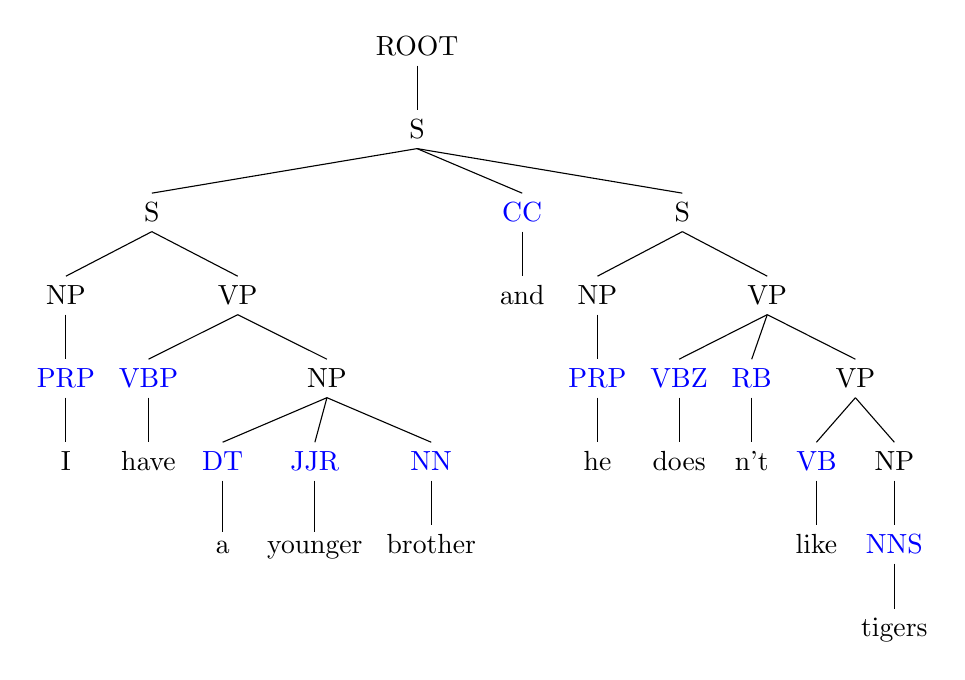
\begin{tikzpicture}
\Tree [.ROOT
        [.S
          [.S
            [.NP [.\textcolor{blue}{PRP} I ] ]
            [.VP
              [.\textcolor{blue}{VBP} have ]
              [.NP [.\textcolor{blue}{DT} a ] [.\textcolor{blue}{JJR} younger ] [.\textcolor{blue}{NN} brother ] ] ] ]
          [.\textcolor{blue}{CC} and ]
          [.S
            [.NP [.\textcolor{blue}{PRP} he ] ]
            [.VP
              [.\textcolor{blue}{VBZ} does ]
              [.\textcolor{blue}{RB} n't ]
              [.VP [.\textcolor{blue}{VB} like ] [.NP [.\textcolor{blue}{NNS} tigers ] ] ] ] ] ] ]
\end{tikzpicture}
\end{quote}

\paragraph*{3. Dependencies}
\begin{quote}
\centering 
\begin{tabular}{l l}
\emph{nsubj}(have-2, I-1) & \emph{root}(ROOT-0, have-2) \\
\emph{det}(brother-5, a-3) & \emph{amod}(brother-5, younger-4) \\
\emph{dobj}(have-2, brother-5) & \emph{cc}(have-2, and-6) \\
\emph{aux}(like-10, does-8) & \emph{neg}(like-10, n't-9) \\
\emph{conj}(have-2, like-10) & \emph{dobj}(like-10, tigers-11)
\end{tabular}
\end{quote}

The above can be graphically represented as
\par
\begin{changemargin}{0.8em}{0.8em}
\begin{dependency}
   \begin{deptext}[column sep=1.3em]
		I \& have \& a \& younger \& brother \& and \& he \& does \& n't \& like \& tigers
		\\
   \end{deptext}
   \depedge[edge unit distance=2ex]{2}{1}{nsubj} \\
   \depedge[edge unit distance=2ex]{5}{3}{det} \\
   \depedge[edge unit distance=2ex]{5}{4}{amod} \\
   \depedge[edge unit distance=2ex]{2}{5}{dobj} \\
   \depedge[edge unit distance=2ex]{2}{6}{cc} \\
   \depedge[edge unit distance=2ex]{10}{8}{aux} \\
   \depedge[edge unit distance=2ex]{10}{9}{neg} \\
   \depedge[edge unit distance=2ex]{2}{10}{conj} \\
   \depedge[edge unit distance=2ex]{10}{11}{dobj}
\end{dependency}
\end{changemargin}

Dependencies are \textit{grammatical relations} between words. For the example above, we see that ``I'' is the subject of the verb ``have'', and ``his'' is a noun possessive modifier of ``name''. The Stanford dependencies manual \citex{man:dependencies} details every dependency used in the Stanford Parser, and all tags used in the Penn TreeBank are found at \url{http://web.mit.edu/6.863/www/PennTreebankTags.html}. There are more than 100 part of speech tags, however to familiarise the reader we list a few of the most common ones:
\begin{itemize}
	\item DT: determiners such as \textit{a}, \textit{the}, \textit{some} etc.
	\item NN: the base tag form for \textbf{nouns}; this class includes subcategories NNS (plural nouns), NNP (proper nouns) and NNPS (plural proper nouns)
	\item VB: base tag form for \textbf{verbs}; includes VBD (past tense), VBN (past participle), VBZ (3rd person singular present) and more
	\item JJ: base tag for \textbf{adjectives}; includes JJR (comparative) and JJS (superlative)
	\item PRP\$: possessive pronouns, such as \textit{his}, \textit{their} etc.
	\item NP: noun phrase tag; a noun phrase is usually composed of a noun and a number of other elements but \textbf{not} a verb. For example ``The small mouse'' is a noun phrase containing a determiner (DT) ``The'', an adjective (JJ) ``small'' and noun (NN) ``mouse''
	\item VP: the verb phrase; it always contains a verb but may also have other tags as we will show shortly
	\item PP: prepositional phrase; begins with a preposition (IN tag), for example
	\begin{center}	
	\Tree [.S
          [.VP
            [.VB Look ]
            [.\textbf{PP} [.IN under ] [.NP [.DT the ] [.NN table ] ] ] ] ] 
	\end{center}
	\item ADJP: adjective phrase; it is formed by an adjective and particles (RB) such as ``very''
	\item ADVP: adverbial phrase; analogously to ADJP it contains an adverb and possibly other tags. The following example shows a sentence consisting of a noun phrase and a verb phrase, with the latter also containing an adverbial phrase
	\begin{center}
	\Tree [.S
          [.NP [.DT A ] [.JJ large ] [.NN cat ] ]
          [.VP
            [.VBD left ]
            [.NP [.DT the ] [.NN house ] ]
            [.ADVP [.RB very ] [.RB slowly ] ] ] ] 
	\end{center}
	\item SQ: inverted yes/no questions e.g. ``Do you like pizza?'' or the main clause of a \textit{wh-}question e.g. ``Which one \textbf{do you want?}''
	\item SBARQ: direct questions, for example ``Which one do you want?''
\end{itemize}

The data obtained from the parser, that is, the three components listed at the beginning of this section (tags, parse and dependencies) are used to create \texttt{Word} objects storing the text word, root, POS tag, position in the sentence, role (dependency) as well as what sentence and dependency group the word belongs to. These \texttt{Word} objects are our own representation of an English word. The root form of each word is obtained using \tech{nltk}'s word Lemmatizer, which, depending on the POS tag of the word, extracts the basic form of the word. For example the verb ``eating'' has root ``eat'' and the noun ``children'' has root ``child''. The word category is extracted from WordNet synsets, essentially sets of synonyms where words are interlinked by lexical relations. The lexical category is what our notion of word category corresponds to.
\begin{table}[H]
\center
\small
\begin{tabular}{rllllllrll}
\hline
 i       & Word   & POS   & S-gp         & WN Category   & Root   &   dep & d-gp   &   target &    neg \\
\hline
  1 & i       & PRP    & S\_1   & undefined       & i             & nsubj  &       & have        &          False         \\
  2 & have    & VBP    & S\_1   & verb.possession & have          & root   &       & tiger       &          False         \\
  3 & a       & DT     & S\_1   & undefined       & a             & det    &       & brother     &          False        \\
  4 & younger & JJR    & S\_1   & adj.all         & young         & amod   &     1 & brother     &          False         \\
  5 & brother & NN     & S\_1   & noun.person     & brother       & dobj   &     1 & have        &          False         \\
  6 & and     & CC     & S     & undefined       & and           & cc     &       & have        &           False         \\
  7 & he      & PRP    & S\_2   & undefined       & he            & nsubj  &       & like        &          False         \\
  8 & does    & VBZ    & S\_2   & verb.social     & do            & aux    &       & like        &          False         \\
  9 & n't     & RB     & S\_2   & undefined       & not           & neg    &       & like        &           True          \\
 10 & like    & VB     & S\_2   & verb.emotion    & like          & root   &       & tiger       &           True          \\
 11 & tigers  & NNS    & S\_2   & noun.person     & tiger         & dobj   &       & like        &          False         \\
\hline
\end{tabular}
\caption{\texttt{Word} objects information}
\label{table:word-obj}
\end{table}
Table \ref{table:word-obj} omits the \texttt{num\_modified} field that indicates whether a word is modified by a number, such as in ``the two \textit{boys}'' where ``two'' modifies ``boys''. Each \texttt{Word} object is stored in an \texttt{EnglishSentence} object in a list. The sentence object also contains information about sentence groups (S-gp in Table \ref{table:word-obj}) with their associated tenses like present, past and future. The syntax tree for the sentence is then processed to replace each String representation of the words with actual \texttt{Word} objects; this way we can directly alter the structure of the sentence whilst retaining all syntactic information.

\subsection{Translation Rules}
\label{rules}
In order to make the system flexible and expandable without having to modify the source code, all parts of the translation module, with the exception of the \texttt{Special Cases}, use external user-defined rules to perform the translation. Taking inspiration in the Apertium system (mentioned in Section \ref{machine translation}), rules can be defined following a standardised format which maps from the source to the target. For the tree transformation rules, we use the Context Free Grammar (CFG) representation of the trees to define source and target mappings. The CFG is a collection of \textit{productions}. The mappings are written following the CFG productions syntax, where the right arrow means the left side symbol \textit{generates} the symbols on the right side. For this reason the symbol used to define the transformation is a vertical line | instead of an arrow $\rightarrow$. Listing \ref{lst:rules} is a snippet of the tree transformation rules used in the application. The full list of rules can be found in Appendix \ref{appendix:rules}.

\begin{lstlisting}[language=Rules,mathescape=true, caption = Tree Transform rules snippet, label = lst:rules]
NP -> JJ NN$\color{red} \sim$ | NP -> NN$\color{red} \sim$ JJ
NP -> <> JJ NN$\color{red} \sim$ | NP -> <> NN$\color{red} \sim$ JJ
NP -> <> ADJP NN$\color{red} \sim$ | NP -> <> NN$\color{red} \sim$ ADJP

// will cover anything like "has died", "was born" i.e. auxiliaries
VP -> VB$\color{red} \sim$ <> VP | VP -> _ <> VP 
// covers "He was sick", "He is tall" etc
VP -> VB$\color{red} \sim$ ADJP <> | VP -> _ ADJP <>

SQ -> VB$\color{red} \sim$ <> | SQ -> _ <>  // removes the "have", "did" etc in questions
SQ -> MD <> | SQ -> _ <>
// handles direct questions introduced by a wh- word or wh-phrase
SBARQ -> WH$\color{red} \sim$ <> | SBARQ -> <> WH$\color{red} \sim$ 
\end{lstlisting}
In the first three lines are some examples of rules that handle noun phrase constructions. The first two are specific cases of sentences where there an adjective is followed by a noun. Let's take \texttt{NP -> <> JJ NN$\sim$ | NP -> <> NN$\sim$ JJ} as an example. The symbol $\sim$ indicates that any tag prefixed by the preceding text can be matched; with NN this includes NNS, NNP, NNPS as shown in the previous section. A noun phrase such as ``The big cats'' can be represented by the tree shown in Figure \ref{fig:cat}a. The diamond $\anything$ (or \texttt{<>} characters in the ASCII format) means any kind of tag(s) will be matched. In this example, $\anything$ will be matched with \textit{DT}, a  determiner. Figure \ref{fig:cat}b shows the result of applying the given rule to the original tree. We can highlight the tags that match the tree nodes to make the process more obvious: 
\[
\textit{NP} \rightarrow \textcolor{red}{\anything} \; \textcolor{blue}{\textit{JJ}} \; \textcolor{com}{\textit{NN$\sim$}} \quad|\quad \textit{NP} \rightarrow \textcolor{red}{\anything} \; \textcolor{com}{\textit{NN$\sim$}} \; \textcolor{blue}{\textit{JJ}}
\]
\begin{figure}[H]
\centering
\begin{subfigure}{.47\textwidth}
  \centering
  \Tree [.NP \edge[red];[.\textcolor{red}{DT} The ] \edge[blue];[.\textcolor{blue}{JJ} big ] \edge[com];[.\textcolor{com}{NNS} cats ] ] 
  \caption{Original syntax tree}
\end{subfigure}%
{\LARGE$\rightarrow$}%
\begin{subfigure}{.47\textwidth}
  \centering
  \Tree [.NP \edge[red];[.\textcolor{red}{DT} The ] \edge[com];[.\textcolor{com}{NNS} cats ] \edge[blue];[.\textcolor{blue}{JJ} big ] ] 
  \caption{Transformed tree}
\end{subfigure}
\caption{Tree transformation using rules: noun phrase}
\label{fig:cat}
\end{figure}
The rule on line 3 acts analogously but with an adjective phrase instead of just an adjective. As was explained earlier, an adjective phrase ADJP could be formed by an adverb + adjective such as ``very big''. Let us  illustrate another example from snippet \ref{lst:rules}, namely \texttt{SQ -> VB$\sim$ <> | SQ -> \_ <>} form line 10, which specifically handles the removal of the auxiliary verb at the beginning of a question. The transformation process is schematised in Figure \ref{fig:qtree}. 
\[
\textit{SQ} \rightarrow \textcolor{red}{\textit{VB$\sim$}} \; \textcolor{blue}{\anything} \quad|\quad \textit{SQ} \rightarrow \textcolor{red}{\nothing} \; \textcolor{blue}{\anything}
\]
\begin{figure}[H]
\centering
\begin{subfigure}{.47\textwidth}
  \centering
  \Tree [.SQ \edge[red];[.\textcolor{red}{VBP} Have ] \edge[blue];[.\textcolor{blue}{NP} [.PRP you ] ] \edge[blue];[.\textcolor{blue}{VP} [.VBN eaten ] ] ] 
  \caption{}
\end{subfigure}%
{\LARGE$\rightarrow$}%
\begin{subfigure}{.47\textwidth}
  \centering
  \Tree [.SQ \edge[red];[.\textcolor{red}{\vphantom{A}$\nothing$} ] \edge[blue];[.\textcolor{blue}{NP} [.PRP you ] ] \edge[blue];[.\textcolor{blue}{VP} [.VBN eaten ] ] ] 
  \caption{}
\end{subfigure}
\caption{Tree transformation using rules: question}
\label{fig:qtree}
\end{figure}

In the above, the underscore symbol \nothing means that any tag in the source (the production on the left of |) at the same position as \nothing in the target (on the right) will be removed. Note that more than 1 rule can be applied to a specific sentence. If we combine the examples from Figure \ref{fig:cat} and \ref{fig:qtree} we obtain the sentence ``Have the big cats eaten?'', which would use both rules to transform the tree as shown in Figure \ref{fig:cat+q}.

\begin{figure}[H]
\centering
\begin{subfigure}{.47\textwidth}
  \centering
  \Tree [.SQ
          [.VBP Have ]
          [.NP [.DT the ] [.JJ big ] [.NNS cats ] ]
          [.VP [.VBN eaten ] ] ] 
  \caption{}
\end{subfigure}%
{\LARGE$\rightarrow$}%
\begin{subfigure}{.47\textwidth}
  \centering
  \Tree [.SQ
          [.VBP \vphantom{A}$\nothing$ ]
          [.NP [.DT the ] [.NNS cats ] [.JJ big ] ]
          [.VP [.VBN eaten ] ] ] 
  \caption{}
\end{subfigure}
\caption{Combined example of tree transformation}
\label{fig:cat+q}
\end{figure}

All of the rules found in the file are created to bring the English sentence syntax tree to a form that most closely resembles that of a BSL sentence. For example knowing that in BSL an \textbf{attributive} adjective (see Section \ref{fig:morphemes}) comes before the noun in order to differentiate it from a \textbf{predicative} adjective we may want to specify mapping (1). Recall that the $\sim$ means any subclass of the tag will be matched. Similarly if we know that a verb phrase begins with \textit{any} verb (as implied by $\sim$) and ends with another verb phrase, then the first verb can be discarded with the \nothing symbol (2). This rule is used for sentence constructs such as ``I have eaten'', corresponding to \slg{me eat} in BSL. Tree transformation rules are written in a descending order according to their complexity to ensure a correct match going from very specific to more generic cases.
\begin{align*}
  \textit{NP} \rightarrow \textit{JJ} \; \textit{NN$\sim$} &\quad|\quad \textit{NP} \rightarrow \textit{NN$\sim$} \; \textit{JJ} \tag{1} \\
  \textit{VP} \rightarrow \textit{VB$\sim$} \; \anything \; \textit{VP} &\quad|\quad \textit{VP} \rightarrow \; \nothing \anything \; \textit{VP} \tag{2}
\end{align*}

Rules for direct translation are similar and are divided in 3 subsets:
\begin{itemize}
	\item Swap: in this category are keywords in a sentence around which words revolve. Strictly speaking, any words that appear \textit{before} the given keyword are placed behind it, and any that appear \textit{after} are placed in front. The keyword itself is then removed from the sentence. For now the only keyword in this category is ``if''. A simple example would be
	\begin{flalign*}
	\text{Tell me if you're okay} = & \text{\slg[q]{you okay} \slg{tell me}} \tag{$\ast$}
	\end{flalign*}
	It is apparent that the words in front of \textit{if} are found at the back of the BSL translation, while the ones following it are at the front and signed with a question facial expression. This is due to rhetoric questions as explained in Section \ref{qneg}.
	\item Multiple words: these are mappings for words that appear together. For example the sequence ``\ldots 25 years old'' matches the rule \textit{year old} $\rightarrow$ \nothing \textit{age}. Again, the \nothing symbol implies deletion.
	\item The rest of the direct mappings are categorised by POS tag. Examples of personal pronouns rules are  \textit{us} $\rightarrow$ \textit{we} and \textit{he} $\rightarrow$ \textit{ix} where \textit{ix} stands for the Index notation as explained in Section \ref{structure}. Here, nouns are also mapped for fingerspelling such as \textit{parents} $\rightarrow$ \textit{-m-m-}.
\end{itemize}
Listing \ref{lst:direct} shows a  snippet of the direct translation rules file; again, the full file is found in Appendix \ref{appendix:rules}. The syntax used here is different: the right arrow $\rightarrow$ defines the mapping i.e. anything on the left maps to the elements on the right, however deletion symbol \nothing keeps the same function.
\begin{lstlisting}[language=Rules2,mathescape=true, caption = Direct translation rules snippet, label = lst:direct]
SWAP
if -> if // moves the sentence after the if before the cause
WORDS
there be -> _ _         // removes the existential there + is
if it -> _ _	           // removes the it (SBAR)
have you -> _ you       // remove any 'have you' questions
...
PRP
i->me
he->ix                  // converts personal pronouns
him->ix                 // to index pointers
she->ix
her->ix
it->_
us->we
they->them
MD
will->_
NNS
parent->-m-f-           // converts word to fingerspelling
NN
mom->-m-m-
...
\end{lstlisting}
In addition to the above there are also two files that complement the translation rules by carrying extra  information. The first contains data obtained from the SignBank website\footnote{\url{http://bslsignbank.ucl.ac.uk}} using a simple HTML web scraper. Figure \ref{fig:signbank}a shows the website data and \ref{fig:signbank}b the formatted result. The Python code for the scraper can be found in Appendix \ref{scraper}. Since each word and word sequence on the website corresponds to a single sign in BSL, we use this data to separate word sequences and match them in the input text. Any sentence that includes a sequence of words found in the \texttt{signbank\_multi.txt} file will see those words combined in a single sign. In \ref{fig:signbank}b, the word ``notice board'' would be signed as one unit and thus become \slg{notice-board} in BSL.
\begin{figure}[H]
\centering
\begin{subfigure}[b]{.5\textwidth}
  \hspace*{-0.5cm}
  \includegraphics[scale=0.55]{chapter4/signbank}
  \caption{}
\end{subfigure}
\qquad
\begin{subfigure}[b]{.4\textwidth}
  \small
    \begin{lstlisting}[language=Rules,mathescape=true]
about time
above all
...
note down
not ever
not exist
not far
not give a damn
not have
notice board
not know
not know person
not like
not matter
not pay attention
...
worn out
would not
year before
\end{lstlisting}
  \caption{}
\end{subfigure}
\caption{SignBank website data and formatted result}
\label{fig:signbank}
\end{figure}
The second file contains \textit{compound} morphemes. Recall from Section \ref{morphology} that a compound morpheme is a sign made up of 2 or more other free morpheme signs. There are only a couple of these available at the time of writing this report and Listing \ref{lst:compounds} shows the contents of this file. The exact usage of this data is explained in more detail in Section \ref{special cases}.
\begin{lstlisting}[language=Rules,mathescape=true, caption = \texttt{compound\_morphemes.txt} file, label = lst:compounds]
blood->red flow
believe->think true
check->see maybe
promise->say true
tiger->zebra animal
\end{lstlisting}

\subsection{System Components}
\subsubsection{Syntax Tree Transforms}

As was discussed in the Background Section \ref{existing methods}, the \tech{TEAM} project uses adjoining tree grammars to convert the English sentences into an intermediate representation from which the ASL translation is obtained. We use a similar approach but instead of an interlingua, we keep the sentence words objects as they are, and after changing the tree structure we obtain our definition of intermediate representation. 

\begin{algorithm}[h]
	\caption{Applying tree transformation rules to the source sentence}
	\label{alg:tree-transforms}
	\begin{algorithmic}[1]
		\Require{transform\_rules is a list of Mapping objects with source and target}
	    \Statex
	    \Function{ApplyTreeTransforms}{\Arg{sentence}}
	    		\Let{new\_productions}{[\;]}
	    		\Let{productions}{\Arg{sentence}.\func{getProductions}}\label{line:getprod}
	    		\\
	    		\For{\Each prod \In productions}
	      		\Let{current\_prod}{prod}
	      		\\
	      		\For{\Each mapping \In transform\_rules}\label{line:2ndloop}
					\Let{source}{mapping.\func{Rebuild}}\label{line:regex}    			
					\Let{match}{\func{Match}(source, current\_prod)}\label{line:match}	      			
	      			\\
		        		\If{match exists}
		          		\Let{source\_i}{\func{makeSourceGroupIndexes}}
		          		\Let{target\_i}{\func{linkSourceTarget}(source, target, source\_i)}\label{line:linksourcetarget}
		        			
		        			\Let{new\_target}{\func{constructTarget}(target, match, target\_i)}\label{line:buildtarget}
						\Let{modified}{\True}
						\Let{current\_prod}{new\_target}	\Comment{\textcolor{com}{Update the production}}	        		
		        		\EndIf
	      		\EndFor
	      		\If{modified is \True}
	      			\Let{prod\_obj}{\func{constructProduction}(prod\_string)}\label{line:construct}
	      			\Let{new\_productions}{new\_productions +prod\_obj}
	      		\Else
	      			\Let{new\_productions}{new\_productions + prod}
	      		\EndIf
			\EndFor
			\Let{grammar}{\func{CFG}(new\_productions)}
			\State \Return{\func{generate}(grammar)}\label{line:return}
	    \EndFunction
	\end{algorithmic}
\end{algorithm}

Let us go through a step-by-step run of this fundamental algorithm in the pipeline; line references are from Algorithm~ \ref{alg:tree-transforms}. Assume we would like to transform the following sentence: ``Have you seen the angry man?'', corresponding to \slg[q]{you see man angry}. Before the function is called, all POS tags in the tree are made unique by adding indices where necessary as this allows us to regenerate the new syntax tree without ambiguities, that is, the CFG will only have one solution. Thus, the syntax tree structure with root word representations would look like this
\begin{center}
\Tree [.ROOT
        [.SQ
          [.\textcolor{blue}{VBP} Have ]
          [.NP [.\textcolor{blue}{PRP} you ] ]
          [.VP [.\textcolor{blue}{VB} see ] [.NP\Sub 1 [.\textcolor{blue}{DT} the ] [.\textcolor{blue}{JJ} angry ] [.\textcolor{blue}{NN} man ] ] ] ] ]
\end{center}
We obtain the productions from the current syntax tree (line \ref{line:getprod}), and for the above example we get the following CFG productions composed of Terminals (words) and Nonterminals (tags):
\begin{align*}
	&\textit{ROOT} \rightarrow \textit{SQ} & & \textit{SQ} \rightarrow \textit{VBP} \quad  \textit{NP} \quad  \textit{VP} \\
	&\textit{VBP} \rightarrow have & & \textit{NP} \rightarrow \textit{PRP} \\
	&\textit{PRP} \rightarrow you & & \textit{VP} \rightarrow \textit{VBN} \quad \textit{NP}\Sub 1 \\
	&\textit{VBN} \rightarrow see & & \textit{NP}\Sub1 \rightarrow \textit{DT} \quad \textit{JJ} \quad \textit{NN} \\
	&\textit{DT} \rightarrow the & & \textit{JJ} \rightarrow angry \\
	&\textit{NN} \rightarrow man
\end{align*}
While iterating through each of the above productions we look for a rule in the list of mappings (transform\_rules) on line \ref{line:2ndloop}. For demonstrative purposes assume production (3) and mapping rule (4) exist.
\begin{gather*}
\text{(production)} \quad \textit{VP} \rightarrow \textit{VB} \quad \textit{VP}\Sub 2 \quad \textit{ADJP} \quad \textit{NNS}\Sub 3 \tag{3}\\
\text{(source)} \quad \textit{VP} \rightarrow \textit{VB} \; \anything \; \textit{NN$\sim$} \quad|\quad \textit{VP} \rightarrow \nothing \; \textit{NN$\sim$} \; \anything \quad \text{(target)} \tag{4}
\end{gather*}
Rule (2) essentially removes the verb and pushes the ending noun to the front of the verb phrase keeping everything else in between. We would then expect the production to become \textit{VP} $\rightarrow$ \textit{NNS}\Sub 3 \textit{VP}\Sub 2 \textit{ADJP}. Since we need to perform a string match between the existing source and source stored in the rules, we rebuild the given source with \texttt{regex} syntax (line \ref{line:regex}). Thus the above source becomes
\[
	\textit{VP}(\Sub?\backslash d?) \rightarrow \textit{VB}(\Sub?\backslash d?)(.*)\textit{NN}([A-Z]*)(\Sub?\backslash d?)\$
\]
The above symbols replace the simple text characters used when writing the rules. Each character has a specific meaning in \texttt{regex}. To begin with, \textit{VP}$(\Sub?\backslash d?)$ will match any string that begins with \textit{VP} \textbf{possibly} followed by an underscore $\Sub$ and a digit $d$. This in fact corresponds to the desired effect of having a tag potentially followed by a unique ID, as is the case for the \textit{angry man} example. Then $\anything$ is replaced by $(.*)$ which will match \textbf{any} string. Finally, the sequence $\textit{NN}([A-Z]*)(\Sub?\backslash d?)\$$ means that any string beginning with \textit{NN} and possibly followed by any number of \textit{letters} and/or followed by an underscore plus a digit will be matched. Any of the following examples will produce a match for the \texttt{regex} rule just described: \textit{NN}, \textit{NN}\Sub1, \textit{NNPS}, \textit{NNPS}\Sub2 etc. The match is then obtained and if successful, generates a group of matches between the two sources. For the production (3), the groups would be (` ',` ',` \textit{VP}\Sub2 \;  \textit{ADJP} ', ` \textit{S} ', ` \Sub 3 ') meaning that \textit{VP} and \textit{VB} yielded an exact match (empty group), the $\anything$ tag matched to \textit{VP}\Sub2 \;  \textit{ADJP} and \textit{NN} matched to the tuple (\textit{S}, \Sub 3). Afterwards,  \textit{Source Match Indexes} (SMI) are created. SMI can be defined as follows: after a match, each element in the source yields match groups specifying the ``differences'' between the original source element and given production. Any group created is assigned an index starting from 1. In addition, any element from the source that is marked with a $\sim$ is linked to a pair of indexes instead of just one since the match can happen for both the subcategory and the unique tag ID. For the current example we find SMI = $[1, 2, 3, (4,5)]$. Figure \ref{fig:smi} schematises the above explanation.

\begin{figure}[H]
\centering
\includegraphics[scale=0.55]{chapter4/SMI}
\caption{Source Match Indexes derived from the match groups}
\label{fig:smi}
\end{figure}

\begin{table}[ht]
\center
\small
\begin{tabular}{l l r r | l l}
Target & Source & Index & Backtrace & TMI & Source Chunks \\
\hline
\textit{VP} & \textit{VP} & 0 & 0 & [ ] & [\textit{VP}, $\rightarrow$, \textit{VB},$\anything$, \textit{NN$\sim$}] \\
\nothing & \textit{VB} & 1 & 0 & [ 1 ] & [$\rightarrow$, \textit{VB},$\anything$, \textit{NN$\sim$}] \\
\textit{NN$\sim$} & $\anything$ & 2 & 0 & [ 1, 2 ] & [$\anything$,\textit{NN$\sim$}] \\
%\multicolumn{1}{c}{\vdots} & \multicolumn{4}{l}{\textit{Setting backtrace}} & \multicolumn{1}{c}{\vdots\vspace{0.2em}}\\
\textit{NN$\sim$} & \textit{NN$\sim$} & 3 & 1 & [ 1, 2 ] & [$\anything$, \textit{NN$\sim$}] \\
%\multicolumn{1}{c}{\vdots} & \multicolumn{4}{l}{\textit{Resetting index and backtrace}} & \multicolumn{1}{c}{\vdots\vspace{0.2em}}\\
\nothing & \nothing & 2 & 0 & [ 1, 2, (4, 5) ] & [$\anything$] \\
 &  & & & [ 1, 2, (4, 5), 3 ] & [ ] \\
\end{tabular}
\caption[Run of the \textsc{LinkSourceTarget} algorithm]{Run of the \textsc{LinkSourceTarget} algorithm. TMI stands for Target Match Indexes.}
\label{table:run}
\end{table}

Source and target elements are linked by rearranging the indexes according to the target (line \ref{line:linksourcetarget}). Table \ref{table:run} shows a run of the linking algorithm for the current example. The index is increased by 1 at each iteration and actually represents the index of the element in the SMI. On the first step \textit{VP} matches \textit{VP}, so we fetch element at position 0 from SMI, 1. Then \nothing matches \textit{VB} (we assume that when \nothing is found, the first element from the source is used) so we fetch element at position 1 from SMI, 2. Then \textit{NN$\sim$} does not match $\anything$, thus we set the backtrace. Backtrace is used to reset the index once the element from the target is found in the source. In fact \textit{NN$\sim$} is found further on, so in the step following we match \textit{NN$\sim$} and fetch element at position 3 from SMI, $(4,5)$. After resetting the index (index - backtrace - 1) we match $\anything$ to $\anything$ and fetch 3 from SMI at position 2, yielding TMI = $[1, 2, (4, 5), 3]$. We then construct the new target by combining the original target (read from the file) to the match groups using the TMI positions. For each tag in the target we find the group of characters at the position from the TMI and append it to said tag (line \ref{line:buildtarget}). Recall that the target for this example is \textit{VP} $\rightarrow$ \nothing \textit{NN$\sim$} $\anything$.
\begin{table}[ht]
\center
\small
\begin{tabular}{l l c c c c c c}
Production & Target & Value in TMI & \multicolumn{5}{c}{Match Group} \\
\hline
 & & & 1 & 2 & 3 & 4 & 5 \\
\hline
[ ] & \textit{VP} & 1 & [\hl{` '} & ` ' & ` \textit{VP}\Sub2 \; \textit{ADJP} ' & ` \textit{S} ' & ` \Sub 2 '] \\

[\textit{VP}] & \nothing & 2 & [\hlgr{` '} & \hl{` '} & ` \textit{VP}\Sub2 \; \textit{ADJP} ' & ` \textit{S} ' & ` \Sub 2 '] \\

[\textit{VP}, $\rightarrow$] & \textit{NN$\sim$} & (4,5) & [\hlgr{` '} & \hlgr{` '} & ` \textit{VP}\Sub2 \; \textit{ADJP} ' & \hl{` \textit{S} '} & \hl{` \Sub 2 '}] \\

[\textit{VP}, $\rightarrow$, \textit{NNS}\Sub3] & $\anything$ & 3 & [\hlgr{` '} & \hlgr{` '} & \hl{` \textit{VP}\Sub2 \; \textit{ADJP} '} & \hlgr{` \textit{S} '} & \hlgr{` \Sub 2 '}] \\ \\

\multicolumn{3}{l}{[\textit{VP}, $\rightarrow$, \textit{NNS}\Sub3, \textit{VP}\Sub2 \textit{ADJP}]} & & & & &
\end{tabular}
\caption[Reconstruction of the target.]{Reconstruction of the target. Yellow highlights the current selection and green those already selected.}
\label{table:rebuild}
\end{table}

From the run in Table \ref{table:rebuild} we find that \textit{VP} is linked to character group 1, however the group is empty, so nothing is appended. Then \nothing is matched to nothing, so we don't insert it in the new target: in fact \nothing means we do not want the Nonterminal to be included in the new production. Then \textit{NN$\sim$} is linked to the tuple (4,5) so we fetch elements from the groups \textit{S} and \Sub3, which are both appended to  \textit{NN} yielding \textit{NNS}\Sub3. Finally $\anything$ is linked to group 3 containing \textit{VP}\Sub2 \textit{ADJP}, which replaces it. The final production is \textit{VP} $\rightarrow$ \textit{NNS}\Sub 3 \textit{VP}\Sub 2 \; \textit{ADJP}, as was expected.

Once all productions have been exhausted and updated we generate a new CFG to build the new transformed syntax tree (line \ref{line:return}). Matching rules for ``Have you seen the angry man?'' are
\begin{align*}
 &\textit{SQ} \rightarrow \textit{VBP} \; \textit{NP} \; \textit{VP} \quad \text{matches} \quad \textit{SQ} \rightarrow \textit{VB$\sim$} \; \anything \quad|\quad \textit{SQ} \rightarrow \nothing \; \anything \\
 &\textit{NP\Sub}1 \rightarrow \textit{DT} \; \textit{JJ} \; \textit{NN} \quad \text{matches} \quad \textit{NP} \rightarrow \textit{DT} \; \anything \; \textit{NN} \quad|\quad \textit{NP} \rightarrow \; \textit{DT} \; \textit{NN} \; \anything
\end{align*}
And the new syntax tree for the intermediate representation is
\begin{center}
\Tree [.ROOT
        [.SQ
          [.NP [.\textcolor{blue}{PRP} you ] ]
          [.VP [.\textcolor{blue}{VB} see ] [.NP\Sub 1 [.\textcolor{blue}{DT} the ]  [.\textcolor{blue}{NN} man ] [.\textcolor{blue}{JJ} angry ] ] ] ] ]
\end{center}

%Here remember to show a diagram of Marshall and their pipeline with word net, parser etc.%

\subsubsection{Direct Translation}
Before applying the direct translation rules as described in Section \ref{rules}, we use SignBank's post-processed data to identify words that may be combined to form a single sign. Note that these are \textbf{not} \textit{compound morphemes} but simply expressions that use multiple words in English, however only require 1 sign in BSL. For example the sentence
\begin{flalign*}
\text{He passed out} = & \text{Index\slg{_1 pass-out}}
\end{flalign*}
While there are signs for both \slg{pass} and \slg{out}, they do not simply combine, instead a completely different sign is used (see Section \ref{qneg}). Refer back to Figure \ref{fig:signbank} for a visualisation of the web data before and after being processed. Words are replaced one by one until exhaustion, the tree representation is dropped and the list of words as a sequence is used instead. At this point we are using an \texttt{IntermediateSentence} object, which contains said list of words and multiple methods to further modify the data representation. It is important to note that any modification to the word is recorded by its root; the original word representation is only kept as a reference.

\subsubsection{Special Cases}
\label{special cases}
Special cases handle transformations that cannot be applied by handwritten external rules. Though it is possible to model them similarly to the tree and direct transformation rules, due to time limitations these are performed through hard-coded rules. The sentence is essentially iterated word by word and if a rule matches the condition it is modified. Rules include and are not limited to:
\begin{itemize}
	\item The replacement of the ``in'' and ``at'' prepositions with ``where'' to change the sentence into a rhetoric question e.g. ``I live in Spain'' = \slg{me live}\slg[q]{where} \slg{-s-p-a-i-n-}
	\item The deletion of the word ``that'' if found in a clause introduced by a subordinating conjunction (SBAR sentence group) e.g. ``You think that I'm sad?'' = \slg[q]{you think me sad}
	\item The creation of a personal pronoun Index whenever a proper noun is the subject of the sentence e.g. ``Mary is my sister'' = \slg{-m-a-r-y-}Index\slg{_1 my sister}
	\item The shifting of time-related words from the \texttt{noun.time} WordNet category towards the front of the sentence to mark the temporal topic (see Section  \ref{tense})
\end{itemize}

After applying the special cases there are a few more operations required before generating the output. Firstly, whenever an Index or possessive pronoun is inserted as \texttt{IX} and \texttt{POSS} respectively, in order to differentiate between multiple actors in the sentence, each is given a unique identifier; in previous examples this was represented as Index, followed by a subscript digit e.g. Index$\slg{_2}$. This problem falls into a separate linguistics field called \textit{coreference resolution} and due to the time restrictions a more primitive method was used to solve it. Essentially, because \texttt{IX} is inserted when a proper noun is found, through the gender of the name and the dependency of the word we can assign the correct ID to each actor. For example
\begin{flalign*}
&\text{Jane loved the letter Mike gave her} = \\
& \text{\slg{-J-A-N-E- IX_1 LOVE LETTER -M-I-K-E- IX_2 GIVE IX_1}}\tag{$\ast$}
\end{flalign*}
The analysis starts with 3 ``empty'' indices \slg{IX} and using the information from the name Jane and the preposition ``her'' we can link them together, assigning the same index to each: $\slg{IX_1}$. The remaining actor in the sentence is Mike which, being a different gender, is assigned another index, $\slg{IX_2}$. 

Secondly we check for compounds using a separate file where each sign (in BSL form) maps to two or more other BSL signs to form compounds. This is done separately from direct translation because the gloss for compound morphemes still represents the original idea: if \slg{promise} is a compound formed by the signs \slg{say} and \slg{true} we still gloss \slg{promise} but sign the other two (see Section \ref{morphology} for details). Any \texttt{Word} object that is a compound is assigned the free morphemes that form it to mark it as such. Taking the example from Table \ref{table:word-obj}, at this point in the processing timeline the \texttt{Word} objects stored in the \texttt{IntermediateSentence} would look like what is depicted in Table \ref{table:inter-word}. Recall that we are interested in the root of each word and not the word values themselves.

\begin{table}[ht]
\center
\small
\begin{tabular}{rlll>{\columncolor[RGB]{204, 230, 255}}lllrlrrl}
\hline
   i & Word    & POS   & S-group  & \textbf{Root}   &   dependency & target   &  neg &  compound   \\
\hline
   0 & i       & PRP   & S\_1   & me       & nsubj &  have     &      False &          \\
   1 & have    & VBP   & S\_1   & have     & root  &  tiger    &      False &          \\
   2 & brother & NN    & S\_1   & brother  & dobj  &  have     &      False &          \\
   3 & younger & JJR   & S\_1   & young    & amod  &  brother  &      False &          \\
   4 & he      & PRP   & S\_2   & ix\_1     & nsubj &  like     &     False &          \\
   5 & n't     & RB    & S\_2   & not-like & neg   &   like     &      True &           \\
   6 & tigers  & NNS   & S\_2   & tiger    & dobj  &  like     &      False &   zebra animal    \\
\hline
\end{tabular}
\caption{\texttt{Word} objects after transformation}
\label{table:inter-word}
\end{table}

\subsubsection{The Container object}
A very important characteristic of BSL is the parallel signing of manual and non-manual features. Not only can facial  expressions and eye gaze change the meaning of a word (Section \ref{eye-gaze}), but they can also be used to set the time (Section \ref{tense}) and differentiate elements in the sentence (Section \ref{facial}). At any given time during signing, a manual sign may be accompanied by 0 or more non-manual features. The following sentence exemplifies this concept:
\begin{flalign*}
&\text{I'm not going to the beach today because it was raining} \tag{a}\\
&= \text{\slg{TODAY ME} \slg[neg]{NOT GO} \slg{BEACH} \slg[q]{WHY} \slg{RAIN}} \tag{$\ast$}
\end{flalign*}
We can see that a question is being asked with \slg{why} and a negation on the action $\slg{not go}$. However, there are more elements that the gloss cannot represent. Let us imagine each non-manual feature as a container of one or more words. Each container may also be within another container. The previous glossed example (a) would be represented as (1) below, however some additional features that are extra information to the signer have to also be stored, thus yielding (2)
\begin{flalign*}
&\texttt{today me (not go)[neg] beach (why)[q] rain} \tag{1} \\
&\texttt{today (me)[hn] (not go)[neg] (beach)[1] ((why)[q] rain)[past]} \tag{2}
\end{flalign*}
In (2), where the extra features are included, \texttt{hn} stands for head nod and \texttt{past} means the action is signed with a past tense-associated expression (explained in Section \ref{non-man}). The \texttt{1} tag also defines a \textit{group} and in the animation module, this will be interpreted as a pause between the signs for \slg{beach} and $\slg{why}$. These \texttt{Container} objects work similarly to a Rose-Tree data structure, where each node (the container) may have 1 or more children that can also be containers themselves. Building of this container data structure is done in the \textsc{setNonManualFeatures} method in the \texttt{IntermediateSentence} class (see Figure \ref{fig:mt-objects}).

\subsubsection{Output}
\label{output}
The final step of the Machine Translation module is to generate the BSL output. At this point all the data is set to a \texttt{BSLSentence} object that contains the methods to create the outputs. Given the example (a) above, the output would consists of 3 separate parts:
\begin{enumerate}
	\item A textual representation: as shown above
	\item A HTML Gloss representation: 
	\begin{lstlisting}[language=HTML, caption = Gloss HTML format]
<span id="0">TODAY</span> 
<span id="1">ME</span> 
<over>
	<span id="2">NOT</span> 
	<span id="3">GO</span>
</over>
<sup> neg</sup> 
<span id="4">BEACH</span>
<over>
	<span id="5">WHY</span>
</over>
<sup> q</sup> 
<span id="6">RAIN</span>
\end{lstlisting}
	\item A JSON format:
	\begin{lstlisting}[language=json, caption = JSON format, label = lst:jsonformat]
(		// manual features and file paths
	[	{ "index": 0, "name": "today", "path": "words/t" },
		{ "index": 1, "name": "me", "path": "words/m" },
		{ "index": 2, "name": "not", "path": "words/n" },
		{ "index": 3, "name": "go", "path": "words/g/verbs" },
		{ "index": 4, "name": "beach", "path": "words/b" },
		{ "index": 5, "name": "why", "path": "words/w" },
		{ "index": 6, "name": "rain", "path": "words/r/verbs" }
	],
	{ 	// non-manual feature animation files
		"anims": ["hn", "neg", "past", "q"] 
	},	// concurrent animation sequence
	[	{ "start": [], "end": [] },
		{ "start": ["hn"], "end": ["hn"] },
		{ "start": ["neg"], "end": [] },
		{ "start": [], "end": ["neg"] },
		{ "start": [], "end": [] },
		{ "start": ["past", "q"], "end": ["q"] },
		{ "start": [], "end": ["past"] }
	],
	[	// modifier activation 
		{ "modifiers": [] }, 
		{ "modifiers": [] }, 
		{ "modifiers": [] }, 
		{ "modifiers": [] }, 
		{ "modifiers": ["pause"] }, 
		{ "modifiers": [] }, 
		{ "modifiers": [] }
	]
)
\end{lstlisting}
\end{enumerate}
The HTML gloss is obtained simply by replacing any occurrence of \texttt{(} with an opening \texttt{over} tag and any occurrence of \texttt{[} with the \texttt{sup} tag, and analogously for the closing tags. The \texttt{over} tag will set an \textit{overline} style on any string within it, while the \texttt{sup} tag sets its content to a \textit{superscript}; this is all done through CSS styles. Individual signs are also wrapped in a \texttt{span} tag with unique IDs corresponding to their position. This is later used by JavaScript to highlight the words in turn as they are signed (see Figure \ref{fig:lofi} in Chapter \ref{design}).

The JSON format contains much more information and it is what is most important for the animation. It is composed of a tuple of 4 objects:
\begin{enumerate}
	\item A list of objects containing an index, the value and path of a word sign. The index is necessary since fingerspelled words are loaded as separate files, though the index of the word is the same for all letters in said word as exemplified below for the sentence \slg{ME THINK -B-O-B- IX_1 NICE}
	\begin{lstlisting}[language=json]
	{ "index": 0, "name": "me", "path": "words/m" }, 
	{ "index": 1, "name": "think", "path": "words/t/verbs" },
	{ "index": 2, "name": "B", "path": "alphabet" }, 
	{ "index": 2, "name": "O", "path": "alphabet" }, 
	{ "index": 2, "name": "B", "path": "alphabet" }, 
	{ "index": 3, "name": "ix_1", "path": "words/i" }, 
	{ "index": 4, "name": "nice", "path": "words/n" }
	\end{lstlisting}
	\item A list of animation files to be loaded for non-manual features: we first load all necessary files to be played in parallel with signs and then arrange them according to the 3rd object.
	\item A list of objects where every object position represents a word in the first list. At any index position, 0 or more non-manual signs may start or stop playing. This parameter is explained more in depth in the upcoming Section \ref{handling-non-man}.
	\item A similar list to the above, but only for modifier features. These include pauses between groups of signs, superlative and comparative adjective modifiers. These are in a separate list because instead of playing different signs concurrently, they modify the sign animation at the index they appear in. The details of sign modifiers are explained in Section \ref{loop}.
\end{enumerate}

\newpage
\section{Animation in ThreeJS}
The following section will discuss the techniques used to animate the virtual agent displaying the signed result. It will cover the creation of a rigged model in Blender, the animation and exporting process into a \texttt{JSON} format and the implementation of the animation engine to display it. Figure \ref{fig:sys-over-anim} highlights the components of the system covered here.

\begin{figure}[H]
	\centering
    \includegraphics[scale=0.75]{chapter4/system-overview-anim}
    \caption{System outline: Animation Engine highlighted}
    \label{fig:sys-over-anim}
\end{figure}	

\subsection{Blender}
Blender is a general purpose CAD application to create 3D renderings and animations. It was extensively used in the Computer Animation course in Michaelmas Term to create complex skeletal animations for the practicals and final exam. In addition, its compatibility with \tech{ThreeJS} through an exporting plug-in made it the best choice of animation software for this project. Blender was used to rig and animate the avatar model that would display the sign animations. 

\subsubsection{Model}
In the Computer Animation course we used an open-source avatar model called Ludwig (Figure \ref{fig:models}a). While it would have been convenient to use it for this project having a pre-set skeleton structure, it was not compatible with the Blender plug-in to export to  \tech{ThreeJS}. Consequently, since it would have been necessary to re-rig the model, the opportunity was taken to find a more ``appealing'' avatar. Elena (displayed in \ref{fig:models}b) is one of the most visually pleasing free models available online (from \url{http://www.blendswap.com/blends/view/69967}). Unfortunately, being also pre-rigged it was also not compatible with \tech{ThreeJS}'s export plug-in. Thus it was necessary to remove the skeletal structure and manually rig the model.

\begin{figure}[H]
\centering
\begin{subfigure}[b]{.5\textwidth}
	\captionsetup{width=0.8\textwidth}
  \centering
  \includegraphics[width=0.8\linewidth]{chapter4/ludwig}
  \caption{}
  \label{fig:ludwig}
\end{subfigure}%
\begin{subfigure}[b]{.5\textwidth}
 \captionsetup{width=0.8\textwidth}
  \centering
  \includegraphics[width=0.8\linewidth]{chapter4/girl}
  \caption{}
  \label{fig:elena}
\end{subfigure}
\caption{Potential 3D avatars - Ludwig and Elena}
\label{fig:models}
\end{figure}

\subsubsection{Skeletal Animation}
Skeletal animation for human figures is the process of constructing a hierarchical bone structure (armature) which is afterwards attached to the overlaying skin, and subsequently animated. \textit{Rigging} describes the action of building a skeleton structure made of virtual bones on a previously modelled object. These bones are not rendered, in the sense that they are not visible in the output, instead they move parts of the object they are assigned to. The skin, technically called \textit{mesh}, of the model object is made of many interconnected vertices that form faces. Groups of faces are assigned a colour or material to modify the appearance of the surface. When rigging a model, each bone is assigned 0 or more vertices and its motion affects the vertex positions according to a specific weight. In Figure \ref{fig:weights} are depicted two virtual bones $i$ and $j$. The square box represents the mesh, each bold dot designates a vertex and the extremes of each dotted triangle represent a joint. The weight that a bone exerts on a vertex decreases as the distance between it and the surrounding vertices increases. This even distribution of weights produces a smooth curve between joint rotations.

\begin{figure}[H]
	\centering
    \includegraphics[scale=0.5]{chapter4/weights}
    \caption[A visualisation of the weight falloff]{A visualisation of the weight falloff; from \url{http://what-when-how.com}}
    \label{fig:weights}
\end{figure}	

The weight distribution is normally performed automatically in Blender once the skeleton structure is completed, though some manual tweaking is required, especially with small or detailed parts of the body such as the hands and the face. When performing the rigging, the model is first imported and is set to a pose-position i.e.\ with the arms pointing sideways away from the body. The skeleton is then constructed bone by bone until a satisfactory freedom of movement is achieved. Given that it must be a hierarchical structure, each non-terminal bone has at least 1 child, except for Inverse Kinematics\footnote{The inverse of Forward Kinematics: given a point or trajectory by the IK bones, the joint angles required for the end effector (the affected bone) to reach a target are automatically calculated.} (IK) bones which indirectly modify the bones they are assigned to. These IK bones include both elbow and hand pairs \texttt{elbow\_IK.R(.L)} and \texttt{arm\_IK.R(.L)} as well as those bones to arc the fingers. Figure \ref{fig:struct}a shows the partial bone structure for the Elena model with an  x-ray view, and Figure \ref{fig:struct}b shows a more exhaustive textual representation. There are additional bones that are not shown in the representation because of redundancy. Nonetheless, to make it clear, each finger bone such as the thumb or index also has 2 more children to simulate the phalanges, and while each finger has 3 specialised bones to move its phalanges, it is also given 1 IK bone to automatically arc the fingers. Figure \ref{fig:hand} shows a close-up screenshot of the hand bones as seen from the Blender viewport with the IK fingers highlighted. Rotating any of those bones closer or further away from the palm of the hand will extend or retract the finger bones.
\begin{figure}[H]
	\centering
    \includegraphics[scale=0.4]{chapter4/hand-zoom}
    \caption[Close up of the avatar hand and underlying bones]{Close up of the avatar hand and underlying bones. In light-blue are IK finger bones.}
    \label{fig:hand}
\end{figure}	
\begin{figure}[H]
\centering
\begin{subfigure}[b]{.6\textwidth}
	\captionsetup{width=0.8\textwidth}
  \centering
  \raisebox{5mm}{
  \includegraphics[width=0.8\linewidth]{chapter4/bone-struct}
  }
  \caption{}
\end{subfigure}%
\begin{subfigure}[b]{.6\textwidth}
 \captionsetup{justification=justified, width=0.5\textwidth}
\footnotesize
\begin{minipage}[t]{0.5\linewidth}
\dirtree{%
.1 Pose.
	.2 hips.
		.3 spine\_01.
			.4 spine\_02.
				.5 neck.
					.6 head.
			.4 shoulder\_L.
				.5 arm\_upper.
					.6 arm\_lower.
						.7 wrist.
							.8 hand.
								.9 thumb.
								.9 index.
								.9 middle.
								.9 ring.
								.9 pinkie.
			.4 shoulder-R.
				.5 \textcolor{red}{as above}.
	.2 eye-target.
}
\end{minipage}
  \caption{}
\end{subfigure}
\caption{3D model bone structure}
\label{fig:struct}
\end{figure}

In Figure \ref{fig:struct}a the bones affected by an IK bone are highlighted in yellow. One may move the \texttt{arm\_IK} bone to lift the hand directly and making the upper and lower arms follow, without having to animate those manually. In other words, IK bones are not attached to any part of the mesh, instead they affect other bones which, in turn, do modify the mesh. This is solely done to assist during the animation process as the \texttt{ThreeJS} plug-in exports animations for all bones regardless of their type. In this particular case the model is missing all leg bones as they are unnecessary within the scope of the project, and their absence does remove some processing load. To animate a bone, we first select it and add a keyframe at a given point in time. Usually a starting keyframe is added for any bone which needs to move from the initial position (both arms down against the sides) to the next. We then select a new position for the bone and set a new keyframe at another time step. The default interpolation value between keyframes is Bezier and was kept that way, since it makes gestures look reasonably more authentic to real-life movements than Linear (Figure \ref{fig:bezier}). Every sign is animated individually and then set to textual format through the JSON exporter plug-in. 

\begin{figure}[H]
	\centering
    \includegraphics[scale=0.9]{chapter4/bezier}
    \caption[Bezier vs. Linear interpolation]{Bezier vs. Linear interpolation. The XYZ axis represents the values of each axis in 3D space.}
    \label{fig:bezier}
\end{figure}	

\subsection{JSON Format and JS Formatter}
When exporting with \texttt{ThreeJS}, one must select all objects that should be included in the \texttt{.json} file, in our case being the mesh and the armature. What results from the export is a large file ($\approx$ 1Mb) containing all the information about the selected objects. The following code snippet shows an overview of the type of data contained in a \texttt{.json} file from the exporter
\begin{lstlisting}[language=json, caption = JSON file for \texttt{ThreeJS}, label = lst:object]
{
	"textures":[...],
	"images":[...],
	"object":{
		"matrix":[1,0,0,0,0,1,0,0,0,0,1,0,0,0,0,1],
		"children":[{
			"name":"body",
			"matrix":[...],
			"type":"Mesh",
			"material":"B29BD348-16B8-30D6-A840-62213DC577EE",
			"geometry":"9142F0FA-03F6-3018-AC00-EF02F6717A93"
		}],
		"type":"Scene"
	},
	"materials":[...],
	"animations":[...],
	"geometries":[{
		"data":{
			"normals":[...],
			"name":"body_plane.001Geometry.1",
			"vertices":[...],
			"influencesPerVertex":2,
			"bones":[...],
			"animations":[...],
			"faces":[...],
			"skinWeights":[...],
			"skinIndices":[...]
		},
		"materials":[...],
		"type":"Geometry"
	}]
}
\end{lstlisting}
The first level of attributes holds information about the scene, the objects it contains and the global variables such as textures, materials and geometries. The \texttt{object} on line 4 defines the base for the mesh of the avatar, the identity matrix and holds the IDs of the materials and geometries that belong to it. \texttt{geometries} on line 17 holds all 3-dimensional objects of the scene; in this case there is only 1. Here are defined all geometrical features like faces and their normals, the vertices that make them up as well as the weights for the bones that affect them: by default only 2 bones can affect a specific vertex (line 22). The other very important information is stored in the \texttt{bones} and \texttt{animations} attributes. We will keep these two aside for now.

As will be explained in more detail in Section \ref{engine}, since we wish to keep model and animations separated to be able to import the animations as and when needed, the above snippet with the model data does not contain any animations. All bones are present but do not move. Any new animation file should thus contain information about \textit{which} bones move, and \textit{when} and \textit{where} they move. Here is where the \tech{JS Formatter} comes into play. As every export of a sign from Blender takes up a lot of space due to the large number of vertices and faces stored in it from the model, it is essential to remove this unnecessary and redundant information and only keep what is truly required. As such, a JSON to JS data compression program was written in \tech{Java} and consists of a simple file chooser application where one can pick a \texttt{.json} file, choose a destination directory, purge it of the extra data and convert that \texttt{.json} file into a \texttt{.js} file\footnote{Strangely, \tech{ThreeJS} reads \texttt{.js} instead of \texttt{.json}. The file structure remains a \tech{JSON} attribute tree, it is only a matter of changing the extension.}. The \tech{ThreeJS} exporter for Blender does not have any sort of options to ignore immobile bones, so the program was written from scratch. This additional step is required to substantially decrease the size of files, essentially compressing them to improve loading times and reduce the network traffic when dealing with animations. The \textsc{Convert} found in the formatter function is described in Algorithm~\ref{alg:convert} and is what deals with the removal of unnecessary data. 

It is interesting that a plug-in with similar functionality does not exist yet, as by removing unnecessary bones we enable the animation of multiple bones in the same skeleton but from different clips. Imagine that two clips, A and B exist, and both contain animations that apply to all bones in the skeleton. Suppose that A contains animations to move the left arm, and B the right arm. However in both cases \textit{all} bones are assigned keyframes because of the way Blender exports JSON files, thus in A the right arm bones are ``animated'' as still i.e. they do not move, and analogously in B for the left arm. If both clips were to be played simultaneously, the animations from each would be assigned a weight of 0.5\footnote{The weight is evenly distributed by the number of animations that apply to a bone. If there were 3 simultaneous clips the weight would be $0.\overline{3}$.}. Hence what would result is an inaccurate animation as all the joint would only complete half of the expected rotations. Thus by removing all the keyframes that do not affect the bones' movements we achieve parallel clip animations with 100\% weights.

\begin{lstlisting}[language=json, caption = \texttt{animation} and \texttt{bones} attributes for the sign \texttt{love}, label = lst:bones-anims]
"bones":[{
		"name":"arm_IK.L",
		"parent":-1,
		"scl":[1,1,1]                       // scale
		"rotq":[0,0,-0,1],                  // rotation quaternion
		"pos":[0.625183,2.37131,0.041744]   // position
	},{ ... },{		                        // all other bones
		"name":"eye.L",
		"parent":8,
		"scl":[1,1,1],
		"rotq":[0.000658,0.711393,-0.702794,-0.000655],
		"pos":[0.167223,0.180856,-0.319214]
}],
"animations":[{
	"hierarchy":[{
		"parent":-1,       // one for each bone, following bones order
		"keys":[{          // one key for each time step
			"pos":[0.625183,2.37131,0.041744],
			"scl":[1,1,1],
			"rot":[0,0,-0,1],
			"time":0	      // time step and above attributes for bone
		},{ ... },{       // all other keys
			"pos":[0.625183,2.37131,0.041744],
			"scl":[1,1,1],
			"rot":[0,0,-0,1],
			"time":1.23333      // last time step
		}]}, {
		"parent":-1,
		"keys":[...]},
		...	                  // all other anim data 
	],
	"name":"love",          // name of particular clip
	"fps": 60,              // frames per second
	"length":1.23333	      // all time steps end on this time
}]
\end{lstlisting}

Listing \ref{lst:bones-anims} details the contents of the \texttt{bones} and \texttt{animations} attributes. We can see on line 21 and 26 that for each time step there are attribute values for each bone: depending on the export options, timesteps can go frame by frames or skip some to reduce file size. Given 60fps and a time length of 1.23333 seconds, the total number of frames is 74. With 11 keys per bone, the information is being updated approximately every 7 frames. From any newly exported file containing the information shown in Listing \ref{lst:object} we get the bones and animations. For each bone and for each keyframe we check if either the location or rotation changes. If it does we keep the bone and animation associated with it, otherwise both are removed. This decreases the file size from 1Mb to approximately 30kb depending on the number of bones moved and duration of the whole clip. The output of \textsc{Convert} is similar to what is shown in Listing \ref{lst:bones-anims} above, in that it contains the \texttt{bones} and \texttt{animation} attributes but includes only the bones that move, and a slightly longer duration (line 8 in Algorithm~\ref{alg:convert}). The file that results from the conversion is what will be read by the animation engine to display the signs.

\begin{algorithm}[H]
	\caption{Removing unnecessary data from animation file}
	\label{alg:convert}
	\begin{algorithmic}[1]
	    \Statex
	    \Function{Convert}{\Arg{file}}
	    		\Let{object}{\func{ReadFile}(\Arg{file})}
	    		\\
	    		\Let{bones}{object.geometries.data.bones}
	    		\Let{animations}{object.geometries.data.animations}
	    		\Let{keyframes}{animations.hierarchy}
	    		\\
	    		\Let{animations.length}{animations.length + 0.3}
	    		\For{\Each $i$ \In bones}
				\Let{still}{\True}
				\Let{location}{keyframes[$i$].keys[0].loc}\Comment{\textcolor{com}{First timestep}}
				\Let{rotation}{keyframes[$i$].keys[0].rotq}
				\\
 				\For{\Each key \In keyframes[$i$].keys}
					\If{location $\neq$ key.loc \Or rotation $\neq$ key.loc}
						\Let{still}{\False}
						\State \Break
					\EndIf
				\EndFor
				\IF{still is \True}
					\State bones.\func{remove($i$)}
					\State animations.\func{remove($i$)}
					\Let{$i$}{$i-$1}
				\EndIf
	    		\EndFor
	    		\State \Return{object(animations, bones)}
	    	\EndFunction
	\end{algorithmic}
\end{algorithm}

\subsection{Animation Engine}
\label{engine}
This section details the JavaScript implementation of the animation engine, including all setup required to build a 3D scene, the animation loop and algorithms to play multiple clips in parallel.\\

The \tech{ThreeJS} website contains a large amount of fully working examples to get started with creating simple 3D scenes. It also includes help on how to import models with animations from external files. The library supports multiple types of file formats, such as Object (\texttt{.obj}), Filmbox (\texttt{.fbx}), Collada (\texttt{.dae}) and more. To begin with, Collada was the chosen data format to store the model and animations, primarily because it is highly flexible whilst keeping a reasonable file size. In fact, Collada uses XML and when storing animations, instead of defining the attributes for each bone at every $n$ timesteps, it only keeps the data for the starting and ending positions at every \textit{keyframe} instead. Unfortunately, whilst developing the engine, it was found that the Collada support for \tech{ThreeJS} was not compatible with the included \texttt{AnimationMixer} module used to play clips. Thus it was dropped for the alternative \tech{JSON} format instead. The Collada testing was performed very early in the development of the project. In fact, many of the 3D techniques described in the next pages had been approved \textit{before} designing the interdependent translation modules. It was deemed advantageous to ensure the correct behaviour of essential elements such as the 3D animation before attempting to create the underlying algorithms.

In WebGL, and consequently in \tech{ThreeJS}, the following elements are required to create and render a scene:
\begin{itemize}
	\item The scene itself: containing \textit{all} 3D objects to be rendered
	\item One or more virtual cameras: these define the viewports of the scene and are what displays the results on the screen
	\item One or more lights	
	\item A renderer: this is what does most of the processing. The WebGL rendering pipeline is schematised in Figure \ref{fig:webgl}, although it is virtually the same for all renderers.
\end{itemize}
In our own implementation of a scene, we find the following objects:
\begin{itemize}
	\item Two directional lights and an ambient light to achieve proper illumination of the avatar
	\item A perspective camera set to view the model from the front by default
	\item A camera target used to point the camera towards the avatar when not in ``fingerspelling'' first person view
	\item The model loaded from an external file
\end{itemize}
An external OpenGL shading language script is included in the HTML file to get a ``skydome'' effect with a white ground and blue sky gradient; this is only done for aesthetic purposes. 
\begin{figure}[H]
	\centering
    \includegraphics[scale=1]{chapter4/webgl}
    \caption{WebGL rendering pipeline}
    \label{fig:webgl}
\end{figure}	
We will now discuss the steps taken by the JavaScript side of the application from initialisation to loading new animations after sending a translation request.
\subsubsection{Scene Initialisation}
Whenever the webpage is first opened, the JavaScript file is called and the scene is built. To begin with, all of the aforementioned elements are created, then the model and the two initial animations, \texttt{idle.js} and \texttt{blinking.js}  are loaded. Loading the model requires two steps: first the file is read and geometry data is separated from the materials data and both are stored in different variables. Next, using the native \texttt{ThreeJS} \texttt{ObjectLoader} method both are combined to create a \texttt{SkinnedMesh}, the technical term used in \tech{ThreeJS} to define a rigged model. The sequence of methods used to load the model is only called once, however any code used to load the initial animations is recalled each time a new translation response is received. The animation loading sequence works as follows:
\begin{enumerate}
	\item Given a url of animation files in the same format as described in Listing \ref{lst:jsonformat}, the data is converted into JSON using \texttt{jQuery}'s \texttt{\$.getJSON} method. The result of this operation is stored in an array of promises\footnote{Defined as ``a single asynchronous operation that hasn't completed yet, but is expected in the future''.}.
	\item Once all promises have been loaded, we iterate over them and three things may happen:
		\begin{enumerate}
			\item If the promise returns a 200 code, then the data was loaded correctly and an \texttt{AnimationClip} object is created and added to the list of clips.
			\item If a 404 code is returned, then the previous method is called again but with the \texttt{/verbs} path removed. This is done because sign files are stored alphabetically and some signs are identical for both the verb and the noun e.g. $\slg{love}$. Recall from Listing \ref{lst:jsonformat} that any sign animation is given as an object with multiple attributes. Using the \texttt{love} example, the animation object for the verb would be  \texttt{\string{ "index": 2, "name": "love", "path": "words/l/verbs" \string}}. However since the sign for \slg{love} is the same for both the verb and noun, we only store one version in the \texttt{words/l} path. See Figure \ref{fig:structure} in the Appendix for a complete structure of the file storage.
			\item If a 404 code is returned twice, then a default \texttt{unknown} sign clip is created. This simply loads an animation displaying the model with a confused facial expression and with both hands and shoulders raised (mimicking a ``I don't know'' look). 
		\end{enumerate}
	\item If the clips are loaded in the initialisation stage, then both are started by calling the \texttt{play()} methods. Otherwise additional methods are called to set up the non-manual features clips.
\end{enumerate}

\subsubsection{Handling non-manual features}
\label{handling-non-man}
As was discussed in Section \ref{output}, the server side returns 3 distinct results: a textual gloss, HTML gloss and JSON representation. In the latter we find information about the sign files and non-manual features that need to be loaded, as well as when they have to be played. Using the second argument of the JSON object, we get the names of all non-manual features required for a specific sentence. The following example
\begin{flalign*}
&\text{I will not go to the beach today because it was raining} \\
&= \text{\slg{TODAY ME} \slg[neg]{NOT GO} \slg{BEACH} \slg[q]{WHY} \slg{RAIN}} \tag{$\ast$}
\end{flalign*}
yields the following arguments
\begin{lstlisting}[language=json]
{	\\ second arg
	"anims": [ "future", "hn", "neg", "past", "q"] 
},
[	\\ third arg
	{ "start": ["future"], "end": [] },
	{ "start": ["hn"], "end": ["hn"] },
	{ "start": ["neg"], "end": [] },
	{ "start": [], "end": ["neg"] },
	{ "start": [], "end": ["future"] },
	{ "start": ["past", "q"], "end": ["q"] },
	{ "start": [], "end": ["past"] }	
]
\end{lstlisting}
The files for \texttt{future}, \texttt{hn}, \texttt{neg}, \texttt{past} and \texttt{q} are obtained and loaded in a similar fashion to what was just discussed. Then using the third argument of the JSON object we replace each newly created \texttt{AnimationClip} object in the data structure so that it can be accessed directly. This operation is performed with a simple loop and an equality check for the clip name. Let us also take the opportunity to better explain this third argument in detail.
\begin{quote}\Large$\quad \overset{0}{\slg{today}} \quad \overset{1}{\slg{me}} \quad\; \overset{2}{\slg{not}} \; \overset{3}{\slg{go}} \quad \overset{4}{\slg{beach}} \quad \overset{5}{\slg{why}} \quad \overset{6}{\slg{rain}}$\end{quote}
\vspace{-5mm}
\begin{figure}[H]
	\centering
    \includegraphics[scale=0.7]{chapter4/concurrent-feats}
    \caption{A BSL sentence and visualised non-manual sequence}
    \label{fig:concurrent-feats}
\end{figure}	
Given a sentence with its container objects set, the concurrent events of non-manual features can be displayed as shown in Figure \ref{fig:concurrent-feats}. Because the animation engine will play one sign at a time in order of appearance, it was necessary to find a data structure that could easily represent the concurrency of  this sequence. The following code shows the above representation in a JSON-compatible format. Each pair in the list contains two inner lists: the first list determines the clips that should start playing and the second those which should stop.
\begin{flalign*}
&\texttt{[ } 
\overset{0}{\ovl{\texttt{( [\textcolor{red}{future}], [ ] )}}}, 
\overset{1}{\ovl{\texttt{( [\textcolor{com}{hn}], [\textcolor{com}{hn}] )}}}, 
\overset{2}{\ovl{\texttt{( [\textcolor{blue}{neg} ], [ ] )}}}, 
\overset{3}{\ovl{\texttt{( [ ], [\textcolor{blue}{neg}] )}}}, \\
&
\overset{4}{\ovl{\texttt{( [ ], [\textcolor{red}{future}] )}}}, 
\overset{5}{\ovl{\texttt{( [\textcolor{red}{q}, \textcolor{blue}{past}], [\textcolor{red}{q}] )}}},
\overset{6}{\ovl{\texttt{( [ ], [\textcolor{blue}{past}] )}}}  
\texttt{ ]}
\end{flalign*}

\subsubsection{Animation Loop}
\label{loop}
After loading all files, the app will be running in a loop, where the same initial animations (\texttt{idle}/\texttt{blink}) are repeated until the user requests to make a translation. The \texttt{animate()} method represents this loop, where booleans are constantly checked to ensure the correct methods are called. There are 4 important tests happening here:
\begin{itemize}
	\item If \texttt{display\_translation} is true, then the boolean \texttt{first\_step} is set to true to activate the clips that were previously loaded. The boolean to display the translation is always set after the translation response has been received and all clips have been loaded.
	\item If any of the step variables is set to true, these being \texttt{first\_step}, \texttt{continuous\_step}, \texttt{final\_step} we check if the clips need to be paused, if the automatic camera setting is enabled and call the methods to play the non-manual features if necessary.
	\item If the cancel button is pressed then all manual and non-manual clip variables are reset.
	\item If we have reached the end of an animation sequence for a particular sentence, the non-manual variables and the interface settings are reset.
\end{itemize}
In addition at the end of this loop there is the call to the \texttt{render()} method, which takes care of updating the camera, the renderer itself, the statistical data such as framerate and the \tech{Tween} library\footnote{\url{http://www.createjs.com/tweenjs}} used for altering modifier clips (see the following Section \ref{non-man-imp}). Whenever a new response from the server arrives, the files are loaded and the sign clips are played in sequence. The full pseudocode for this sequence can be found in Appendix \ref{appendix:loop}. Because the rendering implementation makes constant calls to the \texttt{animate()} method, each step in the display loop must be entered and exited through booleans  otherwise the clips would start playing every time a render call is made, around every 10-15ms \citex{website:render}.

\subsubsection{Non-manual features and modifiers}
\label{non-man-imp}
The loop described above also takes care of calling the methods for playing non-manual features and altering sign animations whenever a modifier is involved. Following the structure described in Section \ref{handling-non-man}, we access the two lists at the index given by the main loop. Then if a clip is found in the \texttt{start} list, it is played. Alternatively, if a clip is found in the \texttt{end} list, it is ended by simply calling the \texttt{fadeOut()} method. The loop for modifiers is separate and analogously to the above it accesses modifier commands from the given index position. The 3 types of modifiers and their effects on animations are shown in Table \ref{table:modifiers}. These effects are applied using the \tech{Tween} library, which allows us to interpolate between any value of any object in JavaScript. To begin with, whenever a modifier is found, the clip assigned to it is paused, and then its time-scale is changed according to the parameter of the modifier. Finally the time-scale is interpolated following a specific delay and easing, though these do not apply to the \textit{pause} modifier.
{\renewcommand{\arraystretch}{2.2}
\begin{table}[H]
\center
\small
\begin{tabular}{|l|c|c|c|c|c|}
\hline
Modifier type & Duration ($\delta$) & Start timescale & End timescale & Delay & Easing\\
\hline
\textit{Comparative} & $\dfrac{(dur - 0.3) \times 1000}{\alpha}$ & $\alpha \times 0.2$ & $\alpha\times 1.5$ & $\dfrac{\delta}{3}$ & Quadratic \\
\hline
\textit{Superlative} & $\dfrac{(dur - 0.3) \times 1000}{\alpha}$ & $\alpha \times 0.1$ & $\alpha\times 1.7$ & $\dfrac{\delta}{1.5}$ & Quartic \\
\hline
\textit{Pause} & $dur += \dfrac{0.2}{\alpha}$ & n/a & n/a & n/a & n/a \\
\hline
\end{tabular}
\caption[Modifier parameters]{Modifier parameters. $dur$ stands for the clip's original duration and $\alpha$ for the global animation speed (range between 0.2-2.0)}
\label{table:modifiers}
\end{table}
}

\newpage
\section{Cross-language Communication with Flask}
\begin{figure}[H]
	\centering
    \includegraphics[scale=0.75]{chapter4/system-overview-flask}
    \caption{System outline: Flask Framework highlighted}
    \label{fig:sys-over-flask}
\end{figure}	

Here we very shortly touch on the communication between JavaScript and Flask. Flask is a microframework for Python that allows bidirectional communication between the server and browser as depicted in Figure \ref{fig:sys-over-flask}. The web application is essentially driven by Python: when the website is uploaded to the Heroku server, the Flask app is created. From here the app \textit{route} is defined. The route that points to the root (line 7 in Listing \ref{lst:flaskp}) contains the method that is called when the root address of the website is entered, which returns the main HTML page where all of the JavaScript imports are made. Then any route created by Flask will point to where JavaScript will send the request from. In this case on line 12 in Listing \ref{lst:flaskp} the route is \texttt{/\_process\_text}, thus JavaScript sends the request to the same address as can be seen on line 5 in Listing \ref{lst:flaskj}. When Python is done processing the data, it is returned and can be further exploited by JavaScript.
\begin{lstlisting}[language=python,caption = {Python and JavaScript communication, Python code}, label = lst:flaskp]
# Initialize the Flask application
app = Flask(__name__)
# Initalise the translating analyser
analyser = Analyser(app=True)

# This route will show a form to perform an AJAX request
@app.route('/')
def index():
    return render_template('indexPage.html')

# Route that will process the AJAX request, result as a proper JSON response (Content-Type, etc.)
@app.route('/_process_text')
def process_text():
    text = request.args.get('input_text', '', type = str)

    sys.stdout = open(devnull, 'w') # suppress printing
    data = analyser.process(text)
    sys.stdout = sys.__stdout__     # reset printing

    # data[0] is gloss, data[1] is html, data[2] is json
    return jsonify(result=(data[1],data[2]))

if __name__ == '__main__':
	app.run()
\end{lstlisting}
\begin{lstlisting}[language=JavaScript,caption = {Python and JavaScript communication, JavaScript code}, label = lst:flaskj]
function beginTranslate(){
    var text = $('input[name="input_text"]').val();
    if (Interface.current_text != text) {
        // get the text from the textbox and send it to python
        $.getJSON('/_process_text', {
            input_text: text
        }, function (data) { 	// on finish request receive data
         	// print the result on screen (gloss)
            Interface.setGloss('bsl', data.result[0]);    
            ... // read clips and other data...
        }
    }
}
\end{lstlisting}

\section{Summary}
In this chapter we discussed the implementation of the Machine Translation module with Python, the different components that make it up and showed how an English sentence is transformed into BSL. The biggest challenge was finding a method that could properly capture all syntactic and semantic elements of BSL. In fact, while the signs themselves are crucial, all non-manual features also play a meaningful role when signing. Furthermore, we described the virtual avatar and how it is animated in Blender, the exporting process and the file format read by JavaScript. Substantial amount of work went into creating complementary software to assist the translation and animation process, such as the HTML scraper for obtaining additional translation data and the \texttt{JS Formatter} to remove unnecessary objects from the Blender animation exports. It was also shown how the animation engine implemented in \tech{ThreeJS} reads the animation files and the way they are displayed in a concurrent sequence when a translation request is made. Finally we touched on the communication between the two modules using the Flask microframework. All of the objectives mentioned in Section \ref{objectives} have been met, however to assess the effectiveness of the implemented system, a formal evaluation is necessary and is discussed in the following chapter. 

%==================================================================================================================================================
%##################################################################################################################################################
%==================================================================================================================================================
%											######## 
%											##       
%											##       
%											#######  
%											      ## 
%											##    ## 
%											 ######  
%==================================================================================================================================================
%##################################################################################################################################################
%==================================================================================================================================================


\chapter{Evaluation}
In this chapter, the evaluation for the system has been divided into two main parts: a linguistics perspective to determine the accuracy of the translation according to a small dataset of reference translations, and a user testing feedback obtained through a survey. In addition, it was possible to get two domains experts: Rachel Sutton-Spence, co-author of the book \textit{The linguistics of British Sign Language: an Introduction} and Adam Schembri, Lecturer in Sociolinguistics at the University of Birmingham to review the system and provide constructive feedback.
\section{Translation}
Before discussing the results for translation accuracy, it is necessary to understand that the current evaluation methods are not entirely fitting when compared to the evaluation of written-written translation. While glosses allow for an easy evaluation approach using string similarity metrics, this representation does not properly encapsulate all the linguistic information that is normally carried through signing \citex{paper:manual-labour}. In fact, the accuracy evaluation only takes into account the exact gloss representation, and ignores all visual-spatial knowledge. In other words, it is possible to inspect the correct use of signs in a translation, including the parallel non-manual features, however it is difficult to automatically evaluate how ``good'' an animation for a particular sign is.

Section \ref{results} gives a comparison of the system's performance and compares those described in the Background Section \ref{existing methods}. However, due to the little amount of formal evaluation results provided, more related work is presented here which, in turn, includes evidence of empirical results. These other projects have not been discussed in the background because their implementation closely follows that of  previously mentioned methods and focuses on the translation of sign languages not derived from English.

\subsection{Evaluation Metrics}
\textbf{BLEU} (BiLingual Evaluation Understudy) is a language-independent precision metric for translation that compares a candidate translation (the hypothesis) with one or more reference sentences \citex{papineni2002bleu}. It is currently the most popular evaluation metric for translation in the field of Computational Linguistics. Based on a modified $n$-gram precision metric $p$, it counts the maximum number of times a word appears in any of the reference translations. The count of each candidate word is then reduced by the maximum count and a penalty is added for brevity of sentences i.e. the shorter the sentence the more impact any incorrect word placement will have. It is typically applied over a whole corpus and not between single sentences, although a Smoothed BLEU method exists for this task \citex{chen2014systematic}. For this metric, the higher the score the better.
\begin{align*}
\text{BLEU} &= \left( \displaystyle\prod_{n=1}^{N} p_n \right) ^{\frac{1}{N}} \times \text{BP} \\[2ex]
\text{where } p &= \dfrac{\text{\% of }n\text{-grams from hypothesis in reference}}{\text{\% of }n\text{-grams in reference}}, \\[2ex]
N &= n\text{-gram size of 1 to 4}\\[2ex]
\text{and BP} &= \text{min}\left( 1, \dfrac{\text{hypothesis length}}{\text{reference length}} \right ) 
\end{align*}
\\
%Surprisingly, of the few implemented works described in the Background, only one uses this metric to compare their system performance. 

\noindent \textbf{WER} (Word Error Rate) works on a word-level (Levenshtein) distance comparison between words in a reference translation and a hypothesis. The score is calculated as the minimum number of editing steps\footnote{By editing steps, we mean any word level transformation from the reference to the hypothesis. For instance, if a word found in the reference is missing in the hypothesis, then that is considered an editing step; steps include substitutions, insertions and deletion of words.} required to go from the reference to the hypothesis. Essentially, any word that is not found in the same place in both sentences adds a penalty to the overall score. While more primitive to BLEU, many translation systems also include this score in their evaluation. For this metric, the lower the score the better.
\[
	\text{WER} = \dfrac{n\text{. of substitutions} + n\text{. of insertions} + n\text{. of deletions}}{\text{reference length}}
\]

\subsection{Short evaluation of previous projects}
\label{previous-results}
Given the very little amount of results provided by previous systems, it is extremely hard to get an accurate idea of how each system compares with one another. None of the rule-based systems included statistical results; nearly all the information was in the form of ``performs reasonably well'' or ``not quite there yet'' which are highly broad and cannot be considered as empirical comparisons. Let us quickly go through a short review of each of the works included in the results below.

\paragraph*{\textsc{MaTrEx} 1} Airport Announcement Accessibility \citex{paper:joining-hands}. This SMT implementation focuses on the airport information domain, where security and general announcements are automatically translated into ISL (Irish Sign Language). An English-ISL bilingual dictionary was created from the data obtained from the ATIS (Airline Travel Information System) dataset. In this paper they provide results for both WER and PER (Position-Independent Error Rate). PER, in contrast to WER, also takes word ordering into account. Their testing reports a minimum WER score of 41.68\%.

\paragraph*{\textsc{MaTrEx} 2} This work is developed by the same authors from the above. Here they use a similar SMT approach but with an improved corpus and more insightful evaluation metrics \citex{paper:manual-labour}. In a similar fashion to the corpus used in our evaluation, they remove sentences that include classifiers from the overall corpus. However they also omit all non-manual features from the evaluation, only keeping them in the animation output. This choice fundamentally affects the accuracy results obtained in the evaluation, and the authors note that it does not allow for a fully accurate representation of sign language and machine translation evaluation. In addition to WER and PER they also provide BLEU. They achieve a maximum BLEU score of 45.64\% and a minimum WER score of 54.56\%.

\paragraph*{LSE MT} Spanish Sign Language \citex{paper:spanish-sl}. This system attempts translation from Spanish to LSE (Lengua de Signos Espa\~nola) and includes both rule and statistical based approaches with empirical results for each. Their domain is limited to Driver's Licences and ID renewals, with a corpus made of around 4000 sentences annotated in glosses and SiGML. Here only a BLEU score is provided for each approach using SiGML, with the best being 68.23\%.

\paragraph{TSL MT} Chinese to Taiwanese SL \citex{paper:wu}. One of the few hybrid systems to include statistical evaluation, it utilises a language specific notation to TSL in a bilingual Chinese-TLS corpus containing around 36.000 sentences. Like the above, it provides a BLEU score in addition to the IBM Model 3 score, a metric which is not considered further in this evaluation being a purely SMT focussed metric. They achieve a score of 86\% for BLEU.

\subsection{Data and Approach}
This system was created using a manually expandable rule-based method since no real BSL corpus exists to this day. All of the previous works have either created their own corpus thanks to very patient expert translators and annotators, or used corpora from very specific domains which would be unsuited for the purpose of this project. However, in order to properly observe the translation accuracy it was necessary to find data to use as reference. The website HandSpeak\footnote{\url{http://www.handspeak.com}} is an American Sign Language learning resource that provides lessons as well as many example sentences. These sentences are formed by a gloss text and an English equivalent text annotation; the text is also accompanied by video. Because the predominant difference between ASL and BSL are the signs themselves, and the structure of sentences stays relatively similar, it was possible to use those sentence pairs as evaluation data. The glossing format used on the website does not quite follow the same one used in our system. For instance all of the sentences marked by a question do not specify exactly which signs are signed with a ``q'' expression and likewise for ``neg''. Some glossed sentences also keep punctuation which is not necessary, and some of the target glosses can be applied to more than one English version. For the example \slg[q]{you feel cold} we find two  translations: ``Are you cold?'' and ``Are you feeling cold?''. 

One of the major advantages of using an online corpus through an HTML scraper is the ability to filter unwanted or corrupted data. Some examples include mathematical symbols such as ``Is 24 $\div$ 4 = 6?'' which our system cannot handle. The use of classifier predicates (see Section \ref{morphology}) in reference sentences also required further manual filtering. These constructs use a very particular notation:
\begin{flalign*}
&\text{The cat looked at the mouse and walked away.} \tag{1}\\
&= \text{\slg{mouse}[left] \slg{cat}[right] \slg{look-at walk-away}[loc]} \\
&\text{A pen on the paper.} = \text{\slg{paper cl-paper pen cl-pen}[loc]}\tag{2}
\end{flalign*}
In example (1) the left and right notation specifies the location of the entities in the syntactic space (see Section \ref{verbs}). In (2) the \slg{cl-}means that the hand assumes the correct handshape for that particular entity. In this case the classifier for paper would be a B hand with the palm facing down to imitate the top of a table, and the pen classifier would be represented by a G hand for long and thin objects. For this reason the sentence pairs extracted from the website have also been split into those \textit{with} classifier predicates and those \textit{without} as it was deemed beneficial to perform accuracy results on respective and combined datasets.

Therefore both the source and target were formatted to comply with our evaluation method. Manual formatting included the removal of inconsistent brackets, insertion of dashes for fingerspelled words e.g. ``Joe'' = \slg{-J-O-E-} and the alteration of the Index notation from \texttt{IX-me} to \texttt{IX\_1} which is the notation employed by this system. Moreover, to ensure that word orderings of the glosses would abide by BSL grammar rules, reference translations in this reduced corpus were adjusted accordingly. Table \ref{table:corpus} shows general information about the corpus used in our evaluation.
\begin{table}[H]
\center
\begin{tabular}{llcc}
\hline
Dataset & Stats & English & BSL \\
\hline
\multirow{ 2}{*}{Basic} & N. of sentences & 185 &\\
& Avg. sentence length & 6.76 & 4.95 \\
& N. of words & 1251 & 916 \\
\hline
\multirow{ 2}{*}{Classifiers} & N. of sentences & 49 &\\
& Avg. sentence length & 8.24 & 6.94 \\
& N. of words & 404 & 340 \\
\hline
\multirow{ 2}{*}{Total} & N. of sentences & 234 &\\
& Avg. sentence length & 7.07 & 5.36 \\
\hline
\end{tabular}
\caption{Test corpus statistical information}
\label{table:corpus}
\end{table}
The following section discusses the accuracy of our system using this corpus. To assure the reader, it is important to point out that the dataset considered for the evaluation was never employed as a \textit{training} set. In other words, the rules written to model the transformations from English to BSL were based on the knowledge previously acquired and not from the sentences in this corpus. After formatting the sentence pairs obtained with the web scraper, they were kept as a ``black box'', in the sense that their grammatical structure was never analysed. Whenever a new rule is added to files read by the translation module, the system accuracy is tested to assess if the rule improves or worsens the overall performance. Should the accuracy be reduced, we can use the aforementioned Smoothed BLEU  \citex{chen2014systematic}  metric to compare sentences that may have been affected. Table \ref{table:smoothed} shows a possible output of the testing using the Smoothed BLEU for individual sentence pairs.
\begin{table}[H]
\center
\footnotesize
\begin{tabular}{l >{\ttfamily}l >{\ttfamily}l c}
\hline
English & {\fontfamily{\familydefault}\selectfont BSL Reference} & {\fontfamily{\familydefault}\selectfont BSL Hypothesis} & S-BLEU Score \\
\hline
Do you need help? & (YOU NEED HELP)[q] & \color{com} (YOU NEED HELP)[q] & 1.0 \\
Have you got any story? & (HAVE ANY STORY)[q] & \color{red} (YOU GET STORY ANY)[q] & 0.502 \\
I like you a lot. & ME LIKE YOU LOT & \color{com} ME LIKE YOU LOT & 1.0 \\
How do you feel? & YOU FEEL (HOW)[q] &  \color{com}YOU FEEL (HOW)[q] & 1.0 \\ 
When did you move in? & YOU MOVE-IN (WHEN)[q] & \color{red} YOU MOVE IN (WHEN)[q] & 0.865 \\
Keep in touch. & CONTINUE TO-CONTACT & \color{red} KEEP IN TOUCH & 0.217 \\
\hline
\end{tabular}
\caption{Output for pair-wise sentence evaluation}
\label{table:smoothed}
\end{table}
The BLEU score for the sentence ``When did you move in?'' can be easily improved by adding a new word sequence \texttt{move in} in the SignBank set to combine them into a single sign. On the other hand we can see from the last sentence ``Keep in touch'' that the reference translation is completely different from the system output as the concept of ``maintaining communication'' uses signs for concrete action of touching to convey an abstract meaning. To achieve the correct translation, this particular sentence would require a targeted direct translation rule.

\section{Accuracy Results}
\label{results}
{\renewcommand{\arraystretch}{1.2}
\begin{table}[H]
\center
\small
\begin{tabular}{lllcc}
\hline
System & Approach & Data/Format & WER (\%) & BLEU (\%) \\
\hline
\multirow{ 2}{*}{LSE MT} & Rule-Based & SiGML & n/a & \cellcolor[rgb]{0.8,1,0}{64.33} \\
& Statistical & SiGML & n/a & \cellcolor[rgb]{0.5,1,0}{68.23} \\
\hline
TSL MT & Hybrid & TSL gloss & n/a & \cellcolor[rgb]{0.2,1,0}{86} \\
\hline
\textsc{MaTrEx} 1 & Statistical & Gloss & \cellcolor[rgb]{0.7,1,0}{41.68} & n/a \\
\hline
\multirow{ 2}{*}{\textsc{MaTrEx} 2} & \multirow{ 2}{*}{Statistical} & Gloss & \cellcolor[rgb]{1,0.4,0}{80.37} & \cellcolor[rgb]{1,0.1,0}{31.84} \\
& & SiGML & \cellcolor[rgb]{1,1,0}{54.46} & \cellcolor[rgb]{1,0.8,0}{45.64} \\  
\hline
\multirow{ 3}{*}{This system} & \multirow{ 3}{*}{Rule-Based} & Gloss (w/o classifiers) & \cellcolor[rgb]{1,1,0}{54.88} & \cellcolor[rgb]{0.8,1,0}{64.26} \\
& & Gloss (only classifiers) & \cellcolor[rgb]{1,0.2,0}{86.34} & \cellcolor[rgb]{1,0.65,0}{40.69} \\
& & Combined & \cellcolor[rgb]{1,0.85,0}{61.47} & \cellcolor[rgb]{0.95,1,0}{57.40} \\ 
\hline
\end{tabular}
\caption[System accuracy results for SL translation]{Accuracy results for SL translation. For WER lower means better, for BLEU higher means better. For clarity, red highlighting represent a poor score and green a favourable score.}
\label{table:results}
\end{table}
}

Table \ref{table:results} shows this system's accuracy compared to those described in Section \ref{previous-results}. The results fully confirm the claim made in Section \ref{machine translation}, stating that \textit{hybrid} approaches usually deliver the highest accuracy. We can also note that the rule-based approach in LSE generates a lower BLEU score than the statistical method on the same data, again confirming what was previously expressed. Our system achieves a decent accuracy on the dataset without classifiers but also a rather large error rate. It is therefore safe to assume that many of the words from the reference translation actually appear in the wrong position, or even do not appear at all, in the hypothesis. We can show this in the following example taken from the corpus:
\begin{center}
\begin{tabular}{ll}
\textbf{English} & I haven't eaten yet \\
\textbf{Reference} & \slg{me eat}\slg[neg]{not-yet} \\
\textbf{Hypothesis} & \slg{me}\slg[neg]{not eat yet}
\end{tabular}
\end{center}
Yielding a Smoothed BLEU score of 76.96\% and WER of 66.6\%. We can visualise the workings of WER in Figure \ref{fig:wer1}. Following the given formula for WER we find a value of $\dfrac{2}{3}$ where the numerator is given by 1 substitution and 1 insertion, and the denominator 3 being the length of the reference. Because we are splitting the two  sentences through single spaces, we also keep all information about the position of non-manual features. The (\slg{not} chunk in the hypothesis shows that a non-manual feature begins at that point. Had the reference translation been \slg{not} at that position, it would have counted as incorrect; this is indeed the desired behaviour.
\begin{figure}[H]
	\centering
    \includegraphics[scale=0.77]{chapter5/wer-example1}
    \caption[WER operations]{WER operations; green lines show correct alignments, and red lines incorrect alignments.}
    \label{fig:wer1}
\end{figure}	

Let us look at another example but with the classifiers dataset (the workings for this example are shown in Figure. \ref{fig:wer2}):
\begin{center}
\begin{tabular}{ll}
\textbf{English} & The police stormed the building \\
\textbf{Reference} & \slg{building cl-building police storm-in} \\
\textbf{Hypothesis} & \slg{police storm building}
\end{tabular}
\end{center}

\begin{figure}[H]
	\centering
    \includegraphics[scale=0.77]{chapter5/wer-example2}
    \caption{WER operations on a classifier predicate sentence}
    \label{fig:wer2}
\end{figure}	
Here we obtain a Smoothed BLEU score of 42.89\% and WER of 100\%. The WER numerator value 4 is given by 2 deletions, 1 substitution and 1 insertion. Since there can be any number of insertions, the overall score may go over 1. It is then clamped back to the max value of 1, or 100\%, although it is not the case here. Note that, from the outset, classifiers were never intended to work with the system, and by looking at the WER score on the classifier-only dataset this becomes apparent. A 86.34\% error rate means that nearly \textit{all} of the words in the reference translation differ from the actual output hypothesis. This is understandable since the translation module is not designed to output gloss with classifier predicates, nor is it capable of resolving classifier predicates from an English sentence. 

Even though the combined score is accounted for, it would be sensible to consider the classifier-free subset as the most significant measure. Once again, it is crucial to remind ourselves that these evaluation scores are highly discrepant as a result of the greatly varying corpora employed by each approach and the divergent decisions made by the authors to omit or incorporate non-manual features.

\section{Survey}

To collect information on the general usability of the application a survey was made public for people to test the website. The survey covered questions on bugs, ease of use of the website, the appeal of the avatar and understandability of the sign animations. All questions from the survey can be found in Appendix \ref{appendix:survey}. There were 43 responses in total with an audience ranging from students to professionals from different backgrounds. All responses were anonymous.

To begin with, a general question about each respondent's fluency in BSL or other equivalent sign language was asked. This was done to get a better insight of how different levels of knowledge judge an online tool. The intention of this question was to distinguish praising comments from someone with a high level of BSL, from someone with no or little knowledge, since the opinion of a skilled user would be more valuable in comparison. 36 participants had no experience in BSL whatsoever, 5 knew a couple of signs, and 2 had enough skill to communicate with the Deaf in every day situations (Level 1-2). Unfortunately no one had a BSL level higher than 3, however that is why the feedback of linguists was specially sought after and their remarks are discussed in Section \ref{feedback}. Around 75\% of the participants with no experience also expressed some sort of interest in BSL, be it just curiosity about how Deaf people communicate or eventually wanting to learn the language.

\subsection{Usability}
Users were asked to specify the browser and device employed to access the website in order to accurately identify bugs and browser specific issues. Figure \ref{fig:devices} shows the given responses; please note that an additional ``Internet Explorer'' field was available, though it was never selected. Following that, they were asked to try the  website a try following some simple guidelines on BSL translation and a short explanation of the interface. 11 out of the 43 participants mentioned experiencing some sort of bugs. Most were related to the laggy animations, probably due to optimisation issues on the users' devices. When comparing the bugs and the devices they appear on, no correlation was found. It is safe to assume that the bugs are not related to implementation issues, but rather appear to be specific to the users' browser or device version. Some users actually misinterpreted the unknown words alert (highlighted in red and accompanied by the shoulder shrug) as bugs. This suggests that some other method of specifying unavailable signs might need to be considered.

\definecolor{bblue}{HTML}{3399FF}
\definecolor{rred}{HTML}{EF3D2A}
\definecolor{yyellow}{HTML}{FDA94E}
\definecolor{ggreen}{HTML}{22C91D}
\definecolor{ppurple}{HTML}{E200E6}

\begin{figure}[H]
\begin{tikzpicture}
    \begin{axis}[
        width  = \textwidth-1cm,
        height = 8cm,
        major x tick style = transparent,
        axis lines*=left,
        ybar=\pgflinewidth,
        bar width=14pt,
        ymajorgrids = true,
        ylabel = {Number of Users},
        %symbolic x coords={Mac,Windows,Linux, iPhone, Android},
        xticklabels =
	    {
	        \strut  Mac,     %% you need comma (,) at the end here and next 2 lines
	        \strut  Windows,
	        \strut  Linux,
	        	\strut  iPhone,
	        	\strut  Android,
	    },
        xtick = {1,2,3,4,5},
        scaled y ticks = false,
        enlarge x limits=0.25,
        ymin=0,
        legend cell align=left,
%        legend style={
%                at={(1,1.05)},
%                anchor=south east
%                column sep=1ex
%        },
		legend style={draw=none, legend columns=-1, column sep=1ex, at={(1,1.1)}},
		nodes near coords
    ]
        \addplot[style={bblue,fill=bblue!50,mark=none}]
            coordinates {(1, 7) (4, 1)};

        \addplot[style={rred,fill=rred!50,mark=none}]
             coordinates {(1, 3) (2, 7) (3, 4) (5, 5)};
             
		\addplot[style={yyellow,fill=yyellow!50,mark=none}]
             coordinates {(1, 2) (2, 3) (3, 3)};

        \addplot[style={ggreen,fill=ggreen!50,mark=none}]
             coordinates {(2, 1)};
             
        \legend{Safari, Chrome, Firefox, Opera, Internet Explorer}
    \end{axis}
\end{tikzpicture}
\caption{Devices and browsers running the website}
\label{fig:devices}
\end{figure}

There was a strong agreement towards the understandability of the interface elements though some people did not grasp the meaning of the ``A'' button for suggestions, even though it was clearly stated in the questionnaire (Figure \ref{fig:chart1}a). When asked about loading times the majority rated them as ``Reasonable'' or ``Short'' (Figure \ref{fig:chart1}b). However there were cases where loading was too long, and this might be due to 2 particular reasons:
\begin{enumerate}
	\item A reduced internet connection will certainly increase loading times as all the scene variables have to be created and the model must be loaded; recall that the avatar file exceeds 1Mb.
	\item If the user was the first to access the website after an idle period, they would have experienced longer loading times. The application is hosted on a free account of the Heroku platform and their terms and conditions state that any free website is given 550 hours of activity every month. All websites are managed by \texttt{dynos}, and any \texttt{dyno} will be set to idle after 30 minutes of inactivity. Thus, if a user accesses the website while the \texttt{dyno} is sleeping, their \textit{initial} loading time will be longer than usual. On the other hand all other delays should not be longer than a couple of seconds.
\end{enumerate}

\def\angle{-45}
\def\radius{2}
\def\cyclelist{{"bblue","rred","ggreen", "yyellow", "ppurple"}}
\newcount\cyclecount \cyclecount=-1
\newcount\ind \ind=-1

\begin{figure}[H]
\centering
\begin{subfigure}[b]{.5\textwidth}
	\captionsetup{width=0.8\textwidth}
  \small
  \centering
  \begin{tikzpicture}
  \foreach \percent/\name in {
  	  62.8/Agree,
  	  32.6/Strongly agree,
	  4.7/Neither agree or disagree
    } {
      \ifx\percent\empty\else               % If \percent is empty, do nothing
        \global\advance\cyclecount by 1     % Advance cyclecount
        \global\advance\ind by 1            % Advance list index
        \ifnum3<\cyclecount                 % If cyclecount is larger than list
          \global\cyclecount=0              %   reset cyclecount and
          \global\ind=0                     %   reset list index
        \fi
        \pgfmathparse{\cyclelist[\the\ind]} % Get color from cycle list
        \edef\color{\pgfmathresult}         %   and store as \color
        % Draw angle and set labels
        \draw[fill={\color!50},draw={\color}] (0,0) -- (\angle:\radius)
          arc (\angle:\angle+\percent*3.6:\radius) -- cycle;
        \node at (\angle+0.5*\percent*3.6:0.7*\radius) {\percent\,\%};
        \node[pin=\angle+0.5*\percent*3.6:\name]
          at (\angle+0.5*\percent*3.6:\radius) {};
        \pgfmathparse{\angle+\percent*3.6}  % Advance angle
        \xdef\angle{\pgfmathresult}         %   and store in \angle
      \fi
    };
\end{tikzpicture}
  \caption{The UI elements are clear and easy to understand}
  \label{}
\end{subfigure}%
\begin{subfigure}[b]{.5\textwidth}
 \captionsetup{width=0.8\textwidth}
  \centering
  \small
  \def\angle{20}
\newcount\cyclecount \cyclecount=-1
\newcount\ind \ind=-1
  \begin{tikzpicture}
  \foreach \percent/\name in {
  	  60.5/Reasonable,
  	  23.3/Short,
  	  4.7/Very short,
  	  7/Long,
  	  4.7/Too long
    } {
      \ifx\percent\empty\else               % If \percent is empty, do nothing
        \global\advance\cyclecount by 1     % Advance cyclecount
        \global\advance\ind by 1            % Advance list index
        \ifnum4<\cyclecount                 % If cyclecount is larger than list
          \global\cyclecount=0             %   reset cyclecount and
          \global\ind=0                   %   reset list index
        \fi
        \pgfmathparse{\cyclelist[\the\ind]} % Get color from cycle list
        \edef\color{\pgfmathresult}         %   and store as \color
        % Draw angle and set labels
        \draw[fill={\color!50},draw={\color}] (0,0) -- (\angle:\radius)
          arc (\angle:\angle+\percent*3.6:\radius) -- cycle;
        \node at (\angle+0.5*\percent*3.6:0.7*\radius) {\percent\,\%};
        \node[pin=\angle+0.5*\percent*3.6:\name]
          at (\angle+0.5*\percent*3.6:\radius) {};
        \pgfmathparse{\angle+\percent*3.6}  % Advance angle
        \xdef\angle{\pgfmathresult}         %   and store in \angle
      \fi
    };
\end{tikzpicture}  
  \caption{Loading times}
  \label{}
\end{subfigure}
\caption[Visualised data for responses on clarity of the UI and loading times]{Visualised data for responses on clarity of the UI and loading times (43 responses)}
\label{fig:chart1}
\end{figure}

\subsection{Effectiveness of the Application}
Aside from the technical evaluation of the website, users were also presented with a section investigating the avatar itself. This included questions such as ``Does the avatar come across as friendly?'' and ``How would you rate the movements of the avatar?''. The vast majority of users (86\%) found the virtual agent appealing and rated its movements as quite natural; the choice was between 1 for completely unnatural and 5 for very natural (Figure \ref{fig:rating}). Interestingly, those people whom did not like the look of the avatar also found its movements unnatural. It was shown in \citex{baylor2009promoting} that ``individuals are more influenced by agents who are similar to themselves with respect to appearance-related characteristics''. This might explain why the participants in our survey highly requested the customisation options to achieve their preferred avatar look. Figure \ref{fig:custom} shows the different elements users would like to be able to edit, with gender being the most requested. Interestingly, for my previous undergraduate project the use of a ``male''\footnote{Quotes are used in this context because the model did not quite resemble a man, but had more of a humanoid look. Though the overall appearance bore more resemblance to a male human and somewhat comparable to the Ludwig model previously shown in Figure \ref{fig:ludwig}.} virtual avatar sparked some controversy as many did not appreciate the inability to choose a female equivalent. This particular preference is also discussed in \citex{baylor2009promoting}, where they suggest that younger individuals, especially students, may find female agents more ``powerful role/social models'', which explains the request for a female avatar. Surprisingly, even when presented with a female agent, gender swap was still the most requested customisation feature.

\begin{figure}[H]
\centering
\begin{subfigure}[b]{.5\textwidth}
	\captionsetup{width=0.8\textwidth}
  \small
  \centering
  \begin{tikzpicture}
    \begin{axis}[
        width  = \textwidth-1cm,
        height = 8cm,
        major x tick style = transparent,
        axis lines*=left,
        ybar=\pgflinewidth,
        bar width=14pt,
        ymajorgrids = true,
        ylabel = {Number of Selections},
        %symbolic x coords={Mac,Windows,Linux, iPhone, Android},
        xticklabels =
	    {
	        \strut  V. Unnatural,     %% you need comma (,) at the end here and next 2 lines
	        \strut  Unnatural,
	        \strut  Neutral,
	        	\strut  Natural,
	        	\strut  V. Natural,
	    },
        xtick = {1,2,3,4,5},
        xticklabel style={rotate=35, anchor=north east, inner sep=0mm},
        scaled y ticks = false,
        enlarge x limits=0.25,
        ymin=0,
        legend cell align=left,
%        legend style={
%                at={(1,1.05)},
%                anchor=south east
%                column sep=1ex
%        },
		legend style={draw=none, legend columns=-1, column sep=1ex, at={(1,1.1)}},
		nodes near coords
    ]
        \addplot[style={bblue,fill=bblue!50,mark=none}]
            coordinates {(1, 1) (2, 2) (3, 13) (4, 19) (5, 8)};
    \end{axis}
\end{tikzpicture}
  \caption{Rating of avatar movements}
  \label{fig:rating}
\end{subfigure}%
\begin{subfigure}[b]{.5\textwidth}
 \captionsetup{width=0.8\textwidth}
  \centering
  \small
\begin{tikzpicture}
    \begin{axis}[
        width  = \textwidth-1cm,
        height = 8cm,
        major x tick style = transparent,
        axis lines*=left,
        ybar=\pgflinewidth,
        bar width=14pt,
        ymajorgrids = true,
        ylabel = {Number of Selections (29 responses)},
        %symbolic x coords={Mac,Windows,Linux, iPhone, Android},
        xticklabels =
	    {
	        \strut  Gender,     %% you need comma (,) at the end here and next 2 lines
	        \strut  Colours,
	        \strut  Body features
	    },
        xtick = {1,2,3,4,5},
        xticklabel style={rotate=35, anchor=north east, inner sep=0mm},
        scaled y ticks = false,
        enlarge x limits=0.25,
        ymin=0,
        legend cell align=left,
%        legend style={
%                at={(1,1.05)},
%                anchor=south east
%                column sep=1ex
%        },
		legend style={draw=none, legend columns=-1, column sep=1ex, at={(1,1.1)}},
		nodes near coords
    ]
        \addplot[style={ggreen,fill=ggreen!50,mark=none}]
            coordinates {(1, 23) (2, 19) (3, 4)};
    \end{axis}
\end{tikzpicture}
  \caption{Additional customisations}
  \label{fig:custom}
\end{subfigure}
\caption[Movement ratings and avatar customisation]{Movement ratings and avatar customisation including skin and hair colour, avatar height etc.}
\end{figure}

Participants were also given the task of setting the ``Show non-manual features'' in the options and attempt to follow the animation at the same time as the notifications (see Figure \ref{fig:non-man-app} for reference). Again, the vast majority was very well able to do so (86\%), with some mentioning the speed change feature to be very useful in that regard.

Of the two users with enough experience that completed the survey, one did not have the possibility to try the website because of a missing graphics driver that prevented the avatar from appearing. To the question about translation accuracy, the other replied with ``There is a fair amount of accuracy'', not being very precise. However they did point out that the flat hand for possessive pronouns is incorrect (ASL uses the flat hand, BSL uses a closed fist) and the fact that London should not be fingerspelled as it has its own sign. These two observations are also discussed by the experts in the next section\footnote{Please note that the two experienced users that participated to the survey may not necessarily be Rachel and Adam, the two consulted linguists.}. 

As was previously mentioned at the beginning of the report, the application was built to make British Sign Language translation available online to those currently learning that would like to practice, and for people who are simply curious about the language. However it is not meant to be used solely as a learning tool. Users were asked if they would recommend the website to someone curious about BSL and to someone learning it, with most people praising the idea of such a tool. To be exact, 90\% would recommend it to someone \textit{curious} about BSL, while 81\% would recommend it to someone \textit{learning} the language. This slight division of opinion might be a result of potential incorrect translations: it would not be wise to use an inaccurate teaching tool, however the occasional mistake can be overlooked if individuals solely use it to get an idea of the language. Looking at the comments linked with the same question, some specifically commended the ease of use and simplicity of the website. The ability to change point of view (from 3rd to 1st person) was well received. Others also liked the fact that the translation is explained, mainly in the additional info, but also thanks to the non-manual features notifications. The experienced user pointed out the range of situations where this tool could come useful
\begin{quote}
``I would recommend this mainly because I think it may have more potential than is first thought. I can think of different applications going forward in the field of deaf education but also for people who are fluent in BSL but who find written text difficult to understand. Of course there would need to be a lot more words etc inputted for this latter use. Then there is also the interest factor. The syntactic changes between English and BSL are interesting and well demonstrated here. It could form one useful way of practising the language if enough words were inputted. The learner could see the sentence first, try to practise it in BSL and then see the Avatar do it as a means of checking progress.''
\end{quote} 

Nonetheless, there were also some negative comments, mainly linked to the lack of vocabulary. This is understandable, as there are many important signs describing emotions and basic actions such as ``drinking'' which are not available. Most signs are simply missing because of time limitations, as each sign animation takes around 5-15 minutes to create depending on the complexity of the hand gestures. On the other hand, many  verbs cannot be added yet because they require syntactic agreement with the object. As was shortly described in Section \ref{structure}, a verb sign may be modified by the object it describes. For instance the action of drinking wine is signed differently from the one drinking coffee because the information about \textit{what} is being consumed is incorporated directly into the handshape of the verb. Thus, it would be wrong to add a sign for ``drinking'' since there is no universal sign for that action: it requires a noun modifier. 

Less significant criticism was aimed at the interface. Some users did not particularly understand the placement of the ``Translate'' button on the far right, and would have instead preferred it near the input box. In addition, the ``A'' button for suggestions was not clear enough and as a result people tried to insert sentences that did not quite work; particularly, names were entered without being capitalised, leading to the system not recognising them as such and thus were not fingerspelled.

Despite the complaints, the application was overall well received by the general public and notably endorsed for its simplicity and innovative application of BSL translation over the browser, making it easily accessible to anyone on a multitude of devices without the need to install it. While there are some changes that could be made to improve its usability, the lack of signs does impose a problem as not many BSL sentences can be generated presently.

\section{Feedback from BSL Linguists}
\label{feedback}
During the time the survey was available, I got in touch with Rachel Sutton-Spence, author of the book employed to learn the linguistics of BSL. Adam Schembri, lecturer in Sociolinguistics at the University of Birmingham was also approached. The website and survey were made available to them to have a first-hand experience and to provide general thoughts about the translation and avatar signer.

Similarly to the general opinion of the public, the aesthetics of the website were well received, although  Rachel expressed that the idea of a virtual signing avatar required some getting used to. This isn't surprising as, in fact, virtual agents used in teaching or training environments are still not universally accepted as comparable to humans  \citex{link2006accessibility}. However one of the main advantages of using a virtual agent is the ability to make it infinitely repeat an exercise or action for the benefit of the user. It is important to understand that depending on the implementation of the avatar and the techniques employed to animate it, a potential lack of realism and restriction on the type of interactions can lead to a degraded user experience. Manually animating humanoid figures requires skills and is often time consuming. That is why many prefer to use motion capture instead; this approach is discussed in more detail in the future work Section \ref{future work}. Adam on the other hand, specifically mentioned that the avatar was understandable and that the animations were very clear.

The rest of the comments were targeted at the translations. Firstly, because the system uses a generic rule for fingerspelling, any proper noun is automatically fingerspelled regardless of the type (person, place, brand etc.). For this reason any sentence that includes a city or country name would actually show that particular word as being fingerspelled, such as Italy = $\slg{-i-t-a-l-y-}$. From the email correspondence with Rachel she expressed the following concern
\begin{quote}
``A blanket rule that all Proper nouns are fingerspelled is not really reliable, though, because there are many proper nouns that do have signs, especially place names. An automated translation system that doesn't know signs for major place names (e.g.\ common European countries, or major UK cities) would be odd.''
\end{quote}
WordNet synsets include multiple subcategories for nouns such as \texttt{noun.animal}. \texttt{noun.person}, \texttt{noun.plant} and many more, including \texttt{noun.location}. With a simple modification to the \texttt{Word} object class it would be possible to perform a boolean check for place names. Naturally, place names would have to be animated as well to be displayed. An additional resource could also come useful since there are some exceptions, such as Essex which is indeed fingerspelled.

Secondly, an issue solely related to the sign representation and that was previously spotted by a participant in the survey, was the incorrect handshape for possessive pronouns such as \textit{yours} or \textit{his}/\textit{hers}. The BSL handshape for personal pronouns is a pointed closed fist, however the current animation displays a flat hand, used in ASL. This was ultimately a personal mistake and through more judicious analysis it could have easily been avoided. Nevertheless, since it is only an issue linked to a sign's representation it can easily be mended by changing the animations for those pronouns that use the \texttt{POSS} sign.

Another issue pinpointed by Rachel had to do with numbers and quantifier signs. For example, any sign modified by a number such as ``three pounds'' where pounds is the currency \pounds, should be combined with the number itself to form $\slg{\pounds-3}$. Similarly, when describing the age of a person we should expect $\slg{age-22}$. Currently, our system displays $\slg{age}$ 22 and $\slg{pound}$ 33, meaning each sign is performed individually. Unfortunately this problem falls within the same category as classifiers and agreement verbs, where the sign animations must be combined in more complex manners than just playing them concurrently. Since it is not  possible, and would be foolish, to animate \textit{all} sign combinations, the system requires additional work to merge complex sign modifiers such as \pounds\ and age with quantifiers and number signs.

Moreover, some signs that utilise the data from SignBank are found to be mishandled. As mentioned by Adam, the sentence ``How are you?'' should result in a single sign \slg[q]{how-are-you}. However because the SignBank step is performed \textit{after} the tree transformations, some rules may apply to the sentence structure and move words to a position where the SignBank composed words do not match any more. Specifically, ``How are you?'' currently yields the BSL translation \slg{you}\slg[q]{how}. The rule that applies here is one covering \textit{Wh-}adverb phrases, where any question starting with a \textit{wh-} word pushes the word at the end of the sentence and marks it with a question tag. While this rule correctly applies to most cases, with \slg{how-are-you} the SignBank lookup would have to be performed before the tree transformations. Another cause of this inaccurate behaviour is the use of the root replacing the word value i.e.\ if ``How are you'' is the source text in the SignBank data, but the root values of each of those words corresponds to ``How is you'', obviously the match will not happen. But as a result of the flexibility and modularity of the system, this can be corrected  easily by moving the SignBank step before the tree transformations, although it would require the system to correctly assign the new single tag to each new aggregated word. Figure \ref{fig:combined} schematises this problem: since 3 words with different POS tags are combined into one, which POS tag should be assigned to the new word?
\begin{figure}[H]
\centering
\begin{subfigure}{.47\textwidth}
  \centering
  \Tree [.ROOT
        [.SBARQ
          [.WHADVP [.WRB How ] ]
          [.SQ [.VBP are ] [.NP [.PRP you ] ] ] ] ]
\end{subfigure}%
{\LARGE$\rightarrow$}%
\begin{subfigure}{.47\textwidth}
  \centering
  \Tree [.ROOT
        [.SBARQ
          [.WHADVP [.\textcolor{red}{?} how-are-you ] ]
          [.SQ [.VBP \vphantom{A}$\nothing$ ] [.NP [.PRP \vphantom{A}$\nothing$ ] ] ] ] ]
\end{subfigure}
\caption{Issue with using SignBank before tree transformations}
\label{fig:combined}
\end{figure}

Finally, Adam mentioned the incorrect sign placement of locations in rhetorical sentence constructs such as
\begin{flalign*}
&\text{I lived in Italy} = \text{\slg{me live}\slg[q]{where} \slg{italy}} \tag{1}\\
&\text{I arrived in London yesterday} = \text{\slg{yesterday me arrive}\slg[q]{where} \slg{london}}\tag{2}
\end{flalign*}
where the supposedly correct translation should be \slg{me live italy} for the example (1). In contrast, Rachel argued that the translation with the \slg[q]{where} pattern (the current system behaviour) is indeed correct. It can be assumed that this is because of the differing modes of use of such sentence constructs between BSL signers.

Overall, the two linguists consulted believe the application is an interesting approach to the translation and transmission of BSL through a virtual agent, though it does not properly represent how some Deaf people sign. This is something that can be improved with the inclusion of more rules and further fine-grained analysis to cover specific cases such as the aforementioned fingerspelling for place names. In addition, more work needs to be done to handle classifier predicates and agreement verbs, though the potential approach for this is reviewed in the following chapter.

\section{Summary}
Through an empirical evaluation we compared this system's translation accuracy to that of previous implementations, attentively discussing differences in approaches, preferred metrics and selected corpora. Because no accurate scheme to assess the correctness of animations exists, more subjective evaluations were also employed. The survey feedback was highly assistive in discovering flaws in the user interaction and web interface in addition to understanding missing features or incorrect behaviour of the system. The device/browser specific question gave a good insight in the type of technology people used to access the tool and results demonstrated its high portability and stable performance. The general feedback also helped to get an idea of the naturalness and intelligibility of animations. The more targeted expert feedback disclosed some overlooked imperfections, such as the incorrect use of the possessive signs and fingerspelling for place names. Some of the suggested improvements can be easily achieved since they require only a few modifications to the overall system. However building a large library of signs will take time and additional changes to accommodate more complex sentences as remarked by the linguists will have to be carefully designed and implemented in the future.

%==================================================================================================================================================
%##################################################################################################################################################
%==================================================================================================================================================
%											 #######  
%											##     ## 
%											##        
%											########  
%											##     ## 
%											##     ## 
%											 ####### 
%==================================================================================================================================================
%##################################################################################################################################################
%==================================================================================================================================================


\chapter{Conclusion}
\section{Discussion}
The work described in this report explored the development of a portable web based translation system from written English to British Sign Language. We presented existing techniques in well established topics such as machine translation, 3D animation and modern web programming and attempted to combine them into an innovative approach to sign language translation. We presented an overview of BSL to give an idea of the differences between written and signed English, as well as to support the decisions made when designing the system. A rule-based method allows us to create grammatical transformations to achieve translation between English and BSL, and while more advanced methods exist such as statistical and hybrid approaches, the final implementation demonstrates potential in solving the interlingual problem of translation. With 3D animation techniques a virtual agent displays the animations of the resulting sign language translation in real time. The available media commands to interact with the avatar make it easy to repeat and carefully understand signs, and the additional settings can be used to adjust the playback to the individual's needs. The resulting system was thus developed successfully, incorporating all the necessary features listed in Section \ref{objectives}. Through an empirical evaluation we assessed the performance of the translation in terms of accuracy, and with the help of both experts and untrained individuals we asserted the correctness of signing from the virtual avatar and the general usability of the website. While there is vast room for improvement and potential expansion, the system is highly regarded as innovative and useful, especially because of its ease of use and attractiveness which could intrigue individuals into learning more about BSL and therefore increase their understanding of the Deaf community. Being a web application, the information generated is available on any modern device and browser, making it remarkably easy to access and applicable to a multitude of situations, including learning and instant translations. The adoption of a user-accessible file management approach makes the system highly extensible. Translation rules can be adjusted to improve the translation while sign animations can continuously be added to expand the available library of signs, without the necessity to modify any of the code.

\section{Difficulties and Achievements}
Some obstacles were encountered throughout the duration of this work, ranging from design decisions of the core system, to technical difficulties with the adopted technologies. These challenges forced me to think differently to what I first expected, and I believe the work produced for this thesis would never have been possible had I not planned in advance exactly what needed to be achieved. One of the most challenging aspects was the extensive reading of BSL linguistics, a crucial step required to correctly develop grammar rules. Had the approach been statistical rather than rule-based, it would still have been necessary to understand the underlying mechanics of sign languages, especially since it would have involved the construction of a large corpus as was done in other works. In retrospect, a statistical or hybrid approach would have probably led to better accuracy and covered more possible translations, however would have required much more preparation, potentially undermining the completion of the equally important animation module. Periodically testing methods and ideas in small scale before implementing them in the final product prevented mistakes that could have caused unexpected outcomes. Namely, the use of the JSON format instead of Collada led to smoother animations without the need to build an interpolation engine from scratch. Had Collada not been tested with \tech{ThreeJS} beforehand, more time would have been consumed modifying the code to migrate to JSON.

The skills learnt in the Computer Animation and Computational Linguistics courses were an immense asset that gave me a useful insight when designing the system. This was also my first large scale programming project using Python, something I had only used minimally in the past. It was also my first web application using JavaScript and Flask. It is satisfying to observe the different modules functioning smoothly after completion, especially considering the high complexity of such a system. The extensive knowledge gained by working on this project made me even more interested in web development and I hope to create other equivalently complex and useful applications in the future, as well as continuing to improve this one.

\section{Future Work}
\label{future work}
The project completed for this thesis lays the foundations for possible future work to either improve the current implementation or build upon it to extend it with additional features.
\subsection{Improvements}
As was mentioned in the previous section, there is definitely room for improvement. On the linguistics side, many rules are still required to get higher accuracy and cover more sentence constructs. Luckily, the current approach is highly extensible thanks to the standardised annotation format, meaning that rules can be added by simply editing the rule files without needing to modify any code. Additional sign animations to display more gestures can also be added independently.

Currently, the \texttt{Special Cases} module still utilises hardcoded rules. To further improve the flexibility of the system, a handwritten rule approach could also be created for it so that procedures that do not fall within the tree transformations or direct translation can be added gradually. Furthermore, many features of BSL still remain untouched. For example \textbf{agreement verbs} are not handled by the translation nor the animation modules. One way of solving this would be using a 3D representation of subject and object whenever an agreement verb is identified, similarly to what was done by Huenerfauth's work on classifier predicates  \citex{thesis:generating-classifiers}. For instance the sentence ``I asked you a question'' translates to $\slg{ME-ASK-YOU QUESTION}$, where \slg{ME} and \slg{YOU} are incorporated in the sign. To achieve this, one could create a basic shape for the \slg{ask} sign and after determining the entities involved, the direction of the arm would follow that of the subjects. In this example the hand would assume the shape of the verb ``ask'' and move from the signer \slg{me} to the position of the partner $\slg{you}$. Naturally things become more complicated when covering \textbf{classifier predicates}. Following Huenerfauth's approach, any entity that is associated with a specific \textit{group} (see Section \ref{structure} for details on classifiers) can be processed separately from the rest of the signs. As was shown in Figure \ref{fig:wer2}, any object involved in a classifier predicate must be represented with a handshape. In this example, the ``building'' entity is signed with the \slg{building} sign and referred to with the ($\slg{cl-building}$) classifier, which is then utilised as default instead of the actual sign for the building entity. Of course, this would involve the development of an entirely separate module to cover these particular constructs, though its inclusion would certainly increase the translation accuracy and variety of sentences the system can handle.

On the other hand, the system could be redesigned with a hybrid approach in mind, using statistical techniques to infer tree transformation and direct translation rules. As a fun but not necessarily  significant interaction improvement, a speech recognition module (perhaps using Google's Cloud Speech API\footnote{\url{https://cloud.google.com/speech/}}) could be set at the beginning of the pipeline to recognise spoken text and automatically translate any recognised sentence. This would be more of an additional feature that users can enable or disable in the settings. Another possible enhancement could be the inclusion of a ``storyboard''-style visual feedback of the resulting translation, where each sign, in addition to being displayed as gloss and animation, is also given as an image depicting the sign in the way it is usually shown in sign language textbooks. It would consist of a still image of the avatar with arrows showing the movements of the hands and face. This could be deemed beneficial as some people may be used to this kind of sign visualisation, and its inclusion would reinforce their understanding of the translation. Being a static representation, it can be ``read'' at the user's own pace rather than at a fixed playback speed. This conceptual visualisation is shown in Figure \ref{fig:storyboard}a and compared to a sign illustration from \texttt{british-sign.co.uk}\footnote{\url{http://www.british-sign.co.uk/british-sign-language/dictionary/}} in Figure \ref{fig:storyboard}b.

\begin{figure}[H]
\centering
\begin{subfigure}[b]{.5\textwidth}
	\captionsetup{width=0.8\textwidth}
  \centering
  \includegraphics[width=0.7\linewidth]{chapter6/animal2}
  \caption{}
\end{subfigure}%
\begin{subfigure}[b]{.5\textwidth}
 \captionsetup{width=0.8\textwidth}
  \centering
  \includegraphics[width=0.7\linewidth]{chapter6/animal1}
  \caption{}
\end{subfigure}
\caption{Static illustrations of the sign \slg{animal}}
\label{fig:storyboard}
\end{figure}

\subsection{Extensions}
Given the number of subfields of Computer Science touched by this work, there are quite a few ideas that come to mind for potential related future projects. Some of these include:
\begin{itemize}
\item The creation of a motion capture to JSON file system. Essentially, one could exploit modern animation techniques for recording body and facial movements to generate sign animations. This method was already employed with ViSiCAST \citex{paper:prototype-text}. Because motion capture often records movement for all visible joints, the main challenge in this project would be the separation between bones that should be considered \textit{essential} to the sign and those that can be discarded to prevent the incorrect weight distribution with playback of simultaneous animations. The output from this system could then be directly used in our web application.

\item A project aimed more towards image processing would involve the automated generation of animation data from pre-synthesised video. An ambitious, yet very interesting concept, it could automatically collect online data from videos of signers (these can be found on websites such as SignBank, SignBSL.com and YouTube) to quickly build a virtual dictionary of signs that can be used in our system. 

\item Finally, the web application itself could eventually be made into a browser add-on. In the introduction of this report, it was stated that reading text is comparatively more challenging for Deaf than for hearing individuals. Hence, given some text on a random website, one could open the add-on and with a window-in-window technique, the translating avatar would appear as a preview and translate the text being displayed to assist native BSL signers. A rendered conceptual visualisation of this idea is shown in Figure \ref{fig:concept}.
\end{itemize}
\begin{figure}[H]
	\centering
    \includegraphics[scale=0.35]{chapter6/concept}
    \caption[Possible browser add-on for the current system]{Possible browser add-on for the current system. The current sentence is highlighted in yellow and the words being signed (approximated) are coloured in pink.}
    \label{fig:concept}
\end{figure}	

{\pagestyle{plain}
%===================== REFREENCES ===================%
%next line adds the Bibliography to the contents page
\addcontentsline{toc}{chapter}{References}
\bibliographystylex{plainurl}
\bibliographyx{references.bib}
\newpage

\addcontentsline{toc}{chapter}{Background Reading}
\nocitesec{*}
\makeatletter
\renewcommand\@biblabel[1]{}
\makeatother
\bibliographystylesec{plainurl}
\bibliographysec{bibliography.bib}


%===================== APPENDIX ===================%

%now enable appendix numbering format and include any appendices
\appendix
\chapter{Translation rules}
\label{appendix:rules}
\textbf{Tree transformations}
\begin{lstlisting}[language=Rules,mathescape=true, caption = tree\_transforms.txt]
NP -> PDT <> | NP -> _ <>
// very specific case
NP -> <> JJ NN$\color{red} \sim$ CC <> NN$\color{red} \sim$ | NP -> NN$\color{red} \sim$ <> JJ CC NN$\color{red} \sim$ <>
NP -> <> JJ JJ NN$\color{red} \sim$ | NP -> <> NN$\color{red} \sim$ JJ JJ
NP -> DT <> NN$\color{red} \sim$ | NP -> NN$\color{red} \sim$ DT <>
NP -> JJ NN$\color{red} \sim$ | NP -> NN$\color{red} \sim$ JJ

NP -> DT RB JJ NN$\color{red} \sim$ | NP -> NN$\color{red} \sim$ DT RB JJ 
NP -> RB JJ NN$\color{red} \sim$ | NP -> NN$\color{red} \sim$ RB JJ
NP -> <> JJ NN$\color{red} \sim$ | NP -> <> NN$\color{red} \sim$ JJ
NP -> <> ADJP NN$\color{red} \sim$ | NP -> <> NN$\color{red} \sim$ ADJP

// will cover anything like "has died", "was born" i.e. auxiliaries
VP -> VB$\color{red} \sim$ <> VP | VP -> _ <> VP 
// covers "He was sick", "He is tall" etc
VP -> VB$\color{red} \sim$ ADJP <> | VP -> _ ADJP <>
VP -> TO <> | VP -> _ <>

PP -> TO NP NP | PP -> _ NP NP
PP -> TO NP | PP -> _ NP

S -> NP ADVP VP | S -> NP VP ADVP

SQ -> VB$\color{red} \sim$ <> | SQ -> _ <>  // removes the "have", "did" etc in questions
SQ -> MD <> | SQ -> _ <>

// handles direct questions introduced by a wh- word or wh-phrase
SBARQ -> WH$\color{red} \sim$ <> | SBARQ -> <> WH$\color{red} \sim$ 

SINV -> MD <> | SINV -> _ <>

WHNP -> WDT NN$\color{red} \sim$ | WHNP -> NN$\color{red} \sim$ WDT 	// handles "which book..."
WHNP -> WHNP <> | WHNP -> <> WHNP
\end{lstlisting}

\newpage
\textbf{Direct translation}
\begin{lstlisting}[language=Rules2,mathescape=true, caption = direct\_translation.txt]
SWAP
if -> if // moves the sentence after the if before the cause
WORDS
there be -> _ _					// removes the existential there + is
if it -> _ _						// removes the it in SBAR
have you -> _ you 				// remove any 'have you' questions
time last -> past time
year old -> _ age
time what -> what time
happy year new -> happy new year
year next -> next-year _
week next -> next-week _
day next -> next-day _
year last -> last-year _
week last -> last-week _
as much as -> same _ _
DT
a->_
an->_
some->_
this->ix
those->ix
that->ix
these->ix
the->_
PRP
i->me
he->ix
him->ix
she->ix
her->ix
it->_
us->we
they->them
POS
's->_
'->_
IN
if->_
because->why
as->_
MD
will->_
NNS
parent->-m-f-
NN
mom->-m-m-
mum->-m-m-
mother->-m-m-
dad->-d-d-
father->-d-d-
CC
and->_ 			// remove and conjunction
$
$->dollar
RB
o'clock->time
VB
be->_
VBD
be->_
VBZ
be->_
VBG
be->_
VBP
be->_
\end{lstlisting}

\textbf{SignBank multi-words}
\begin{lstlisting}[language=Rules,mathescape=true, caption = signbank\_multi.txt]
about time
above all
add up
adhesive tape
adultery adulterous
air force
alarm bell
alcoholic drink
all day
// ... 680 more lines 
will do
wind someone up
wipe out
work hard
work out
world record
worn out
would not
year before
\end{lstlisting}

\chapter{Additional algorithms and Code}
\label{appendix:algos}

\section{Data Extraction from the Stanford Parser}
\label{retrieval}
Upon launching the web-app, a \texttt{Parser} object is created in Python and depending on the availability of the online interface of the Stanford Parser, the object will either act as an HTML scraper on the interface's source, or create a local version of the parser (Listing \ref{lst:parser}).

\begin{lstlisting}[language=Python, caption = Parser object creation from the Stanford implementation, label = lst:parser]
from nltk.parse.stanford import StanfordParser, StanfordDependencyParser

class Parser:
    def __init__(self, app=False):
        # first check accessibility of stanford website
        status_code = 0
        try:
            initRequest = requests.post(
              "http://nlp.stanford.edu:8080/parser/index.jsp",timeout=5) 
            # test that the parser still available
            status_code = initRequest.status_code

        except requests.ConnectionError:
            print "Not online, using offline parser"
        except requests.exceptions.Timeout:
            print "Response too slow, using offline parser"

        if (status_code == 200): # online
            self.online = True
        else:
            self.online = False

            # setup necessary variables to create local stanford parser
                os.environ['STANFORD_PARSER'] = APP_PARSER
                ...
            # setup tree parser
            self.parser = StanfordParser()
            # setup dependency parser
            self.dependency_parser = StanfordDependencyParser()
\end{lstlisting}
Because each version yields the same data but in a different format, the \texttt{parse} method executes the correct code for each situation. As can be seen on line 7 in Listing \ref{lst:parse}, when the Stanford Parser is online we use the \tech{BeautifulSoup} library to scrape the HTML page where the result of the request is displayed. From there we obtain the 3 essential objects: the tagged sentence (line 10), the parse tree (line 12) and the dependencies (line 14). On the other hand, if we are using a local version then the methods differ as the parser will return objects instead of raw text. These objects have to comply to the same format, thus they are altered accordingly.

\begin{lstlisting}[language=Python, caption = Obtaining the data from the remote or local parser, label = lst:parse]
def parse(self, sentence):
    if(self.online):
       r =requests.post("http://nlp.stanford.edu:8080/parser/index.jsp",
          data={'parse': 'Parse', 
          'parserSelect': 'English', 
          'query': sentence})
       soup = BeautifulSoup(r.text, "html.parser")
       tagging = ' '.join(soup.find("div", 
                    {"class": "parserOutputMonospace"}).text.split())
       parseTree = ' '.join(soup.find_all("pre", 
                    {"class": "spacingFree"})[0].text.split())
       parseTree = nltk.Tree.fromstring(parseTree)

       dependencies = soup.find_all("pre", 
                    {"class": "spacingFree"})[1].text.split('\n')             
       return [tagging, parseTree, dependencies]  # complete result
    else:
       parseTree = list(self.parser.raw_parse(sentence))[0]

       dependencies_res = self.dependency_parser.raw_parse(sentence)
       dependencies_res = dependencies_res.next()
       dependencies = list(triples_alt(dependencies_res))

       leaves = list(parseTree.subtrees(lambda t: t.height() == 2))
       tagging = ''
       for pair in leaves:
          # remove brackets then split tag/word
          txt = str(pair).strip("()").split() 
             tagging += txt[1]+'/'+txt[0] + ' '
          tagging = tagging[:-1]
          return [tagging, parseTree, dependencies]
\end{lstlisting}

\newpage
\section{HTML scraper for the SignBank data retrieval}
\label{scraper}
\begin{lstlisting}[language=Python, caption = Python code for parsing the SignBank website, label = lst:parse]
url = 'http://bslsignbank.ucl.ac.uk/dictionary/search/?'
query = 'query='
page = '&page='
file = open('signbank_multi.txt', 'w')
for letter in ascii_uppercase:
    index = 1
    prevWords = ''
    while(True): # until we haven't found all the words for this letter
        html = requests.get(url+query+letter+page+str(index))
        
        soup = BeautifulSoup(html.text, "html.parser")
        table = soup.find('div', {'id':'searchresults'})
        
        soup = BeautifulSoup(table.text, 'html.parser')
        words = filter(lambda x: len(x) > 0,soup.get_text().split('\n'))
        
        if words == prevWords:
            break
        print words
        prevWords = words
        
        for w in words:
            # we only save those words that make up 1 sign
            if len(w.split(' ')) > 1:
                file.write(w+'\n')
        index += 1
file.close()
\end{lstlisting}

\newpage
\section{Main animation sequence loop}
\label{appendix:loop}
\begin{minipage}{1\linewidth}
\begin{algorithm}[H]
\small
	\begin{algorithmic}[1]
		\Require{fade\_counter is a variable to access individual clip objects in the clip list}
		\Require{mixer is an object that directly modifies the clips for fading, playing etc.}
		\Require{URL.manual contains the data to load clips (index, name, path)}
		\State
		\Function{playSequence}{}
			\Let{clip}{clips[fade\_counter]}
			\IF{first\_step is \True}
				\State mixer.\func{Set}(clip)\Comment{Loop, reset and play clip}
				\State \func{modifierLoop}(fade\_counter)\label{line:modcall}
				\State fade to next clip
				\\
				\Let{fade\_counter}{fade\_counter + 1}
				\Let{first\_step}{\False}
				\Let{continuous\_step}{\True}
				\\
			\EndIf
			\If{continuous\_step is \True}
				\If{URL.manual length $>$ 1}
					\If{clip.time $>$ clip.duration}
						\State pause clip
						\\
						\If{clip.name = next clip.name}
							\State change next clip.name
						\EndIf
						\State mixer.\func{Set}(clip)
						\State \func{modifierLoop}
						\State \func{checkCompounds}
						\State fade to next clip
						\\
						\If{fade\_counter = URL.manual length}\Comment{Sequence end}
							\Let{continuous\_step}{\False}
							\Let{final\_step}{\True}
						\EndIf
						\Let{fade\_counter}{fade\_counter + 1}
					\EndIf
				\Else				
					\Let{continuous\_step}{\False}
					\Let{final\_step}{\True}
				\EndIf
				
			\EndIf
			\If{final\_step is \True}
				\If{clip.time $>$ clip.duration}
					\State pause clip
					\State mixer.\func{Reset}
					\State fade to init clips\Comment{Idle clip}
					\\
					\State reset HTML gloss
					\Let{final\_step}{\False}
				\EndIf
			\EndIf
		\EndFunction
	\end{algorithmic}
	\caption{Clips animation sequence}
	\label{alg:sequence}
\end{algorithm}
\end{minipage}

\chapter{Screenshots and Project Structure}
\label{appendix:misc}
	
\begin{figure}[h]
	\centering
	\includegraphics[scale=0.4]{appendix/future}
    \includegraphics[scale=0.4]{appendix/neg}
    \caption{``Show non-manual features'' enabled playback}
    \label{fig:non-man-app}
\end{figure}	

\begin{figure}[h]
	\centering
    \includegraphics[scale=0.45]{appendix/fpv}
    \caption{First person view of the avatar when fingerspelling the letter ``J''}
    \label{fig:fpv}
\end{figure}
\begin{figure}[h]
	\centering
    \includegraphics[scale=0.45]{appendix/3rd}
    \caption{3rd person view at the same time as what is displayed in Figure \ref{fig:fpv}}
    \label{fig:3rd}
\end{figure}

\DTsetlength{0.2em}{3em}{0.2em}{0.4pt}{2.2pt}
\begin{figure}
\vspace*{-2cm}
\small
\dirtree{%
.1 BSL.
	.2 \textcolor{blue}{app.py}.
	.2 static.
		.3 lib.
			.4 js.
			.4 nltk-data.
			.4 stanford-parser.
		.3 py.
			.4 \textcolor{blue}{analyser.py}.
			.4 \textcolor{blue}{bleu.py}.
			.4 \textcolor{blue}{parser.py}.
			.4 \textcolor{blue}{rules.py}.
			.4 \textcolor{blue}{sentence.py}.
			.4 \textcolor{blue}{test.py}.
			.4 \textcolor{blue}{utils.py}.
			.4 unit-test.
				.5 \textcolor{blue}{classifier-test-set.txt}.
				.5 \textcolor{blue}{test-set.txt}.
				.5 \textcolor{blue}{train-set.txt}.
		.3 res.
			.4 animations.
				.5 alphabet.
				.5 init.
					.6 \textcolor{blue}{blinking.js}.
					.6 \textcolor{blue}{idle.js}.
					.6 \textcolor{blue}{unknown\_0.js}.
				.5 non-manual.
					.6 \textcolor{blue}{future.js}.
					.6 \textcolor{blue}{hn.js}.
					.6 \textcolor{blue}{neg.js}.
					.6 \textcolor{blue}{past.js}.
					.6 \textcolor{blue}{q.js}.
				.5 numbers.
				.5 words.
					.6 a.
						.7 \textcolor{blue}{age.js}.
						.7 verbs.
							.8 \textcolor{blue}{arrive.js}.
					.6 $\ldots$.
					.6 z.
			.4 css.
			.4 fonts.
			.4 model.
			.4 rules.
		.3 threejs.
	.2 templates.
		.3 \textcolor{blue}{index.html}.
	.2 venv.
}
\caption[File structure of the project]{File structure of the project; files are highlighted in blue}
\label{fig:structure}
\end{figure}

\chapter{Survey Questions}
\label{appendix:survey}

\begin{enumerate}
	\item \textbf{What is your level of knowledge of sign language (BSL, ASL or equivalent)? Choose one.}
	\begin{enumerate}
		\item[$\bigcirc$] No experience at all
		\item[$\bigcirc$] Limited knowledge (Know a few signs and/or the alphabet)
		\item[$\bigcirc$] Level 1-2 (Enough skills to communicate with Deaf people in a range of everyday situations)
		\item[$\bigcirc$] Level 3-4 (Enough skill to interact on a regular basis with Deaf people in a work environment)
		\item[$\bigcirc$] Level 6 (Enough skill to work professionally with Deaf people e.g. teachers in BSL, translators etc.)
	\end{enumerate}
	
	\textbf{If you answered No experience, have you ever been curious about BSL or Sign languages in general?}
	\begin{enumerate}
		\item[$\bigcirc$] Yes
		\item[$\bigcirc$] No
	\end{enumerate}
\end{enumerate}

	\begin{mdframed}[hidealllines=true,backgroundcolor=blue!5] \par At this point the users are directed to the website \url{translate.nicmosc.com} where the application is hosted. They are given some guidelines on what is available and a short introduction to the application in general.
	\end{mdframed}

\begin{enumerate}[resume] % to resume	
	\item \textbf{Did you notice any bugs? If no skip this question. Otherwise choose any of the following.}
	\begin{enumerate}
		\item[$\Box$] Website did not load
		\item[$\Box$] The spinning wheel does not stop and no animation is shown
		\item[$\Box$] The animations are laggy (frames per seconds are low)
		\item[$\Box$] The website crashed
		\item[$\Box$] Other: \dotfill
	\end{enumerate}
	\item \textbf{Please specify the device and browser you are currently using.
If you found bugs and switched browsers/device, select the former. Please click only 1 of the following.}
	\begin{center}
	{\renewcommand{\arraystretch}{1.6}
	\begin{tabular}{c c c c c c}
	& Safari & Chrome & Firefox & Opera & Internet Explorer \\
	Mac computer & $\bigcirc$ & $\bigcirc$ & $\bigcirc$ & $\bigcirc$ & $\bigcirc$ \\
	\hline
	Windows computer & $\bigcirc$ & $\bigcirc$ & $\bigcirc$ & $\bigcirc$ & $\bigcirc$ \\
	\hline	
	Linux computer & $\bigcirc$ & $\bigcirc$ & $\bigcirc$ & $\bigcirc$ & $\bigcirc$ \\
	\hline	
	iPhone & $\bigcirc$ & $\bigcirc$ & $\bigcirc$ & $\bigcirc$ & $\bigcirc$ \\
	\hline	
	Android phone & $\bigcirc$ & $\bigcirc$ & $\bigcirc$ & $\bigcirc$ & $\bigcirc$ \\
	\end{tabular}
	}
	\end{center}
	
	\item \textbf{The interface buttons are clear and it is easy to understand what they do. To what extent do you agree with this statement?}
	\begin{enumerate}
		\item[$\bigcirc$] Strongly agree
		\item[$\bigcirc$] Agree
		\item[$\bigcirc$] Neither agree or disagree
		\item[$\bigcirc$] Disagree
		\item[$\bigcirc$] Strongly disagree
	\end{enumerate}
	
	\item \textbf{Does the avatar come across as friendly?}
	\begin{enumerate}
		\item[$\bigcirc$] Yes
		\item[$\bigcirc$] No
		\item[$\bigcirc$] Kind of
	\end{enumerate}	
	
	\item \textbf{If you answered ``No'' or ``Kind of'' above, why do you think so?}
	\par \dotfill
	
	\item \textbf{How would you rate the movements of the avatar?}
	\begin{center}
	\begin{tabular}{c c c c c c c}
	& 1 & 2 & 3 & 4 & 5 & \\
	Very unnatural & $\bigcirc$ & $\bigcirc$ & $\bigcirc$ & $\bigcirc$ & $\bigcirc$ & Very natural
	\end{tabular}
	\end{center}
	
	\item \textbf{Do you think the avatar should be customisable? If so select which options you would like to see. Otherwise skip this question.}
	\begin{enumerate}
		\item[$\Box$] Gender
		\item[$\Box$] Colours (skin, clothes, hair etc.)
		\item[$\Box$] Body features (height, weight, arms length etc.)
		\item[$\Box$] Other \dotfill
	\end{enumerate}
	
	\item \textbf{How did you feel about loading times?}
	\par{\fontsize{10}{12}\selectfont Please note that depending on your internet connection and other factors (such as the machine you are using) may affect this. Also the first translation will always take longer than the following ones.}
	\begin{enumerate}
		\item[$\bigcirc$] Very short
		\item[$\bigcirc$] Short
		\item[$\bigcirc$] Reasonable
		\item[$\bigcirc$] Long
		\item[$\bigcirc$] Too long
	\end{enumerate}		
	
	\item \textbf{You were able to follow the animation along with the text output and notifications. To what extent do you agree with this statement?}
	\begin{enumerate}
		\item[$\bigcirc$] Agree
		\item[$\bigcirc$] Disagree
		\item[$\bigcirc$] Other: \dotfill
	\end{enumerate}

	\item \textbf{If you feel that you have enough experience to comment on the accuracy of the translation (in terms of adequacy and fluency), please do so below.}
	\par{\fontsize{10}{12}\selectfont Adequacy is a rating of how much information is transferred between the original and the translation, and fluency is a rating of how good the translation is.}
	\par \dotfill
	
	\item \textbf{Would you recommend this website to someone curious about sign language?}
	\begin{enumerate}
		\item[$\bigcirc$] Yes
		\item[$\bigcirc$] No
		\item[$\bigcirc$] Don't care
	\end{enumerate}

	\item \textbf{Why?}
	\par \dotfill
	
	\item \textbf{Would you recommend this website to someone who is learning BSL?}
	
	\begin{enumerate}
		\item[$\bigcirc$] Yes
		\item[$\bigcirc$] No
		\item[$\bigcirc$] Don't care
	\end{enumerate}

	\item \textbf{Why?}
	\par \dotfill
	
	\item \textbf{Finally, what did you like about the application?}
	\par \dotfill
	
	\item \textbf{What did you dislike?}
	\par \dotfill
	
\end{enumerate}
\cleardoublepage}

\end{document}
